\chapter{Extended Results} \label{ch:eresult}
\section{Set Estimation}\label{eresult:setest}
Estimation using the techniques with different models are illustrated using data for one vehicle in the dataset in this chapter. Results show that the true state is always bounded by the set of estimation. For acceleration, there is no true measurement because the acceleration of the tracked vehicle is absent in the dataset.
\FloatBarrier
\subsection{Segment Minimization using F-Radius}
\FloatBarrier
\begin{figure}[h]
\begin{subfigure}{.5\linewidth}
\centering
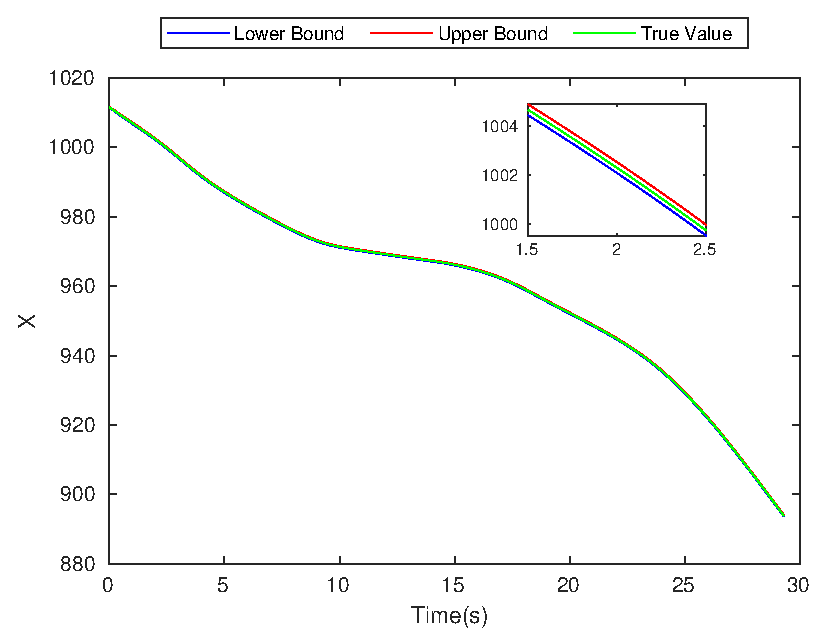
\includegraphics[width=\linewidth]{figures/Frad/s3cvSMX}
\end{subfigure}
\begin{subfigure}{.5\linewidth}
\centering
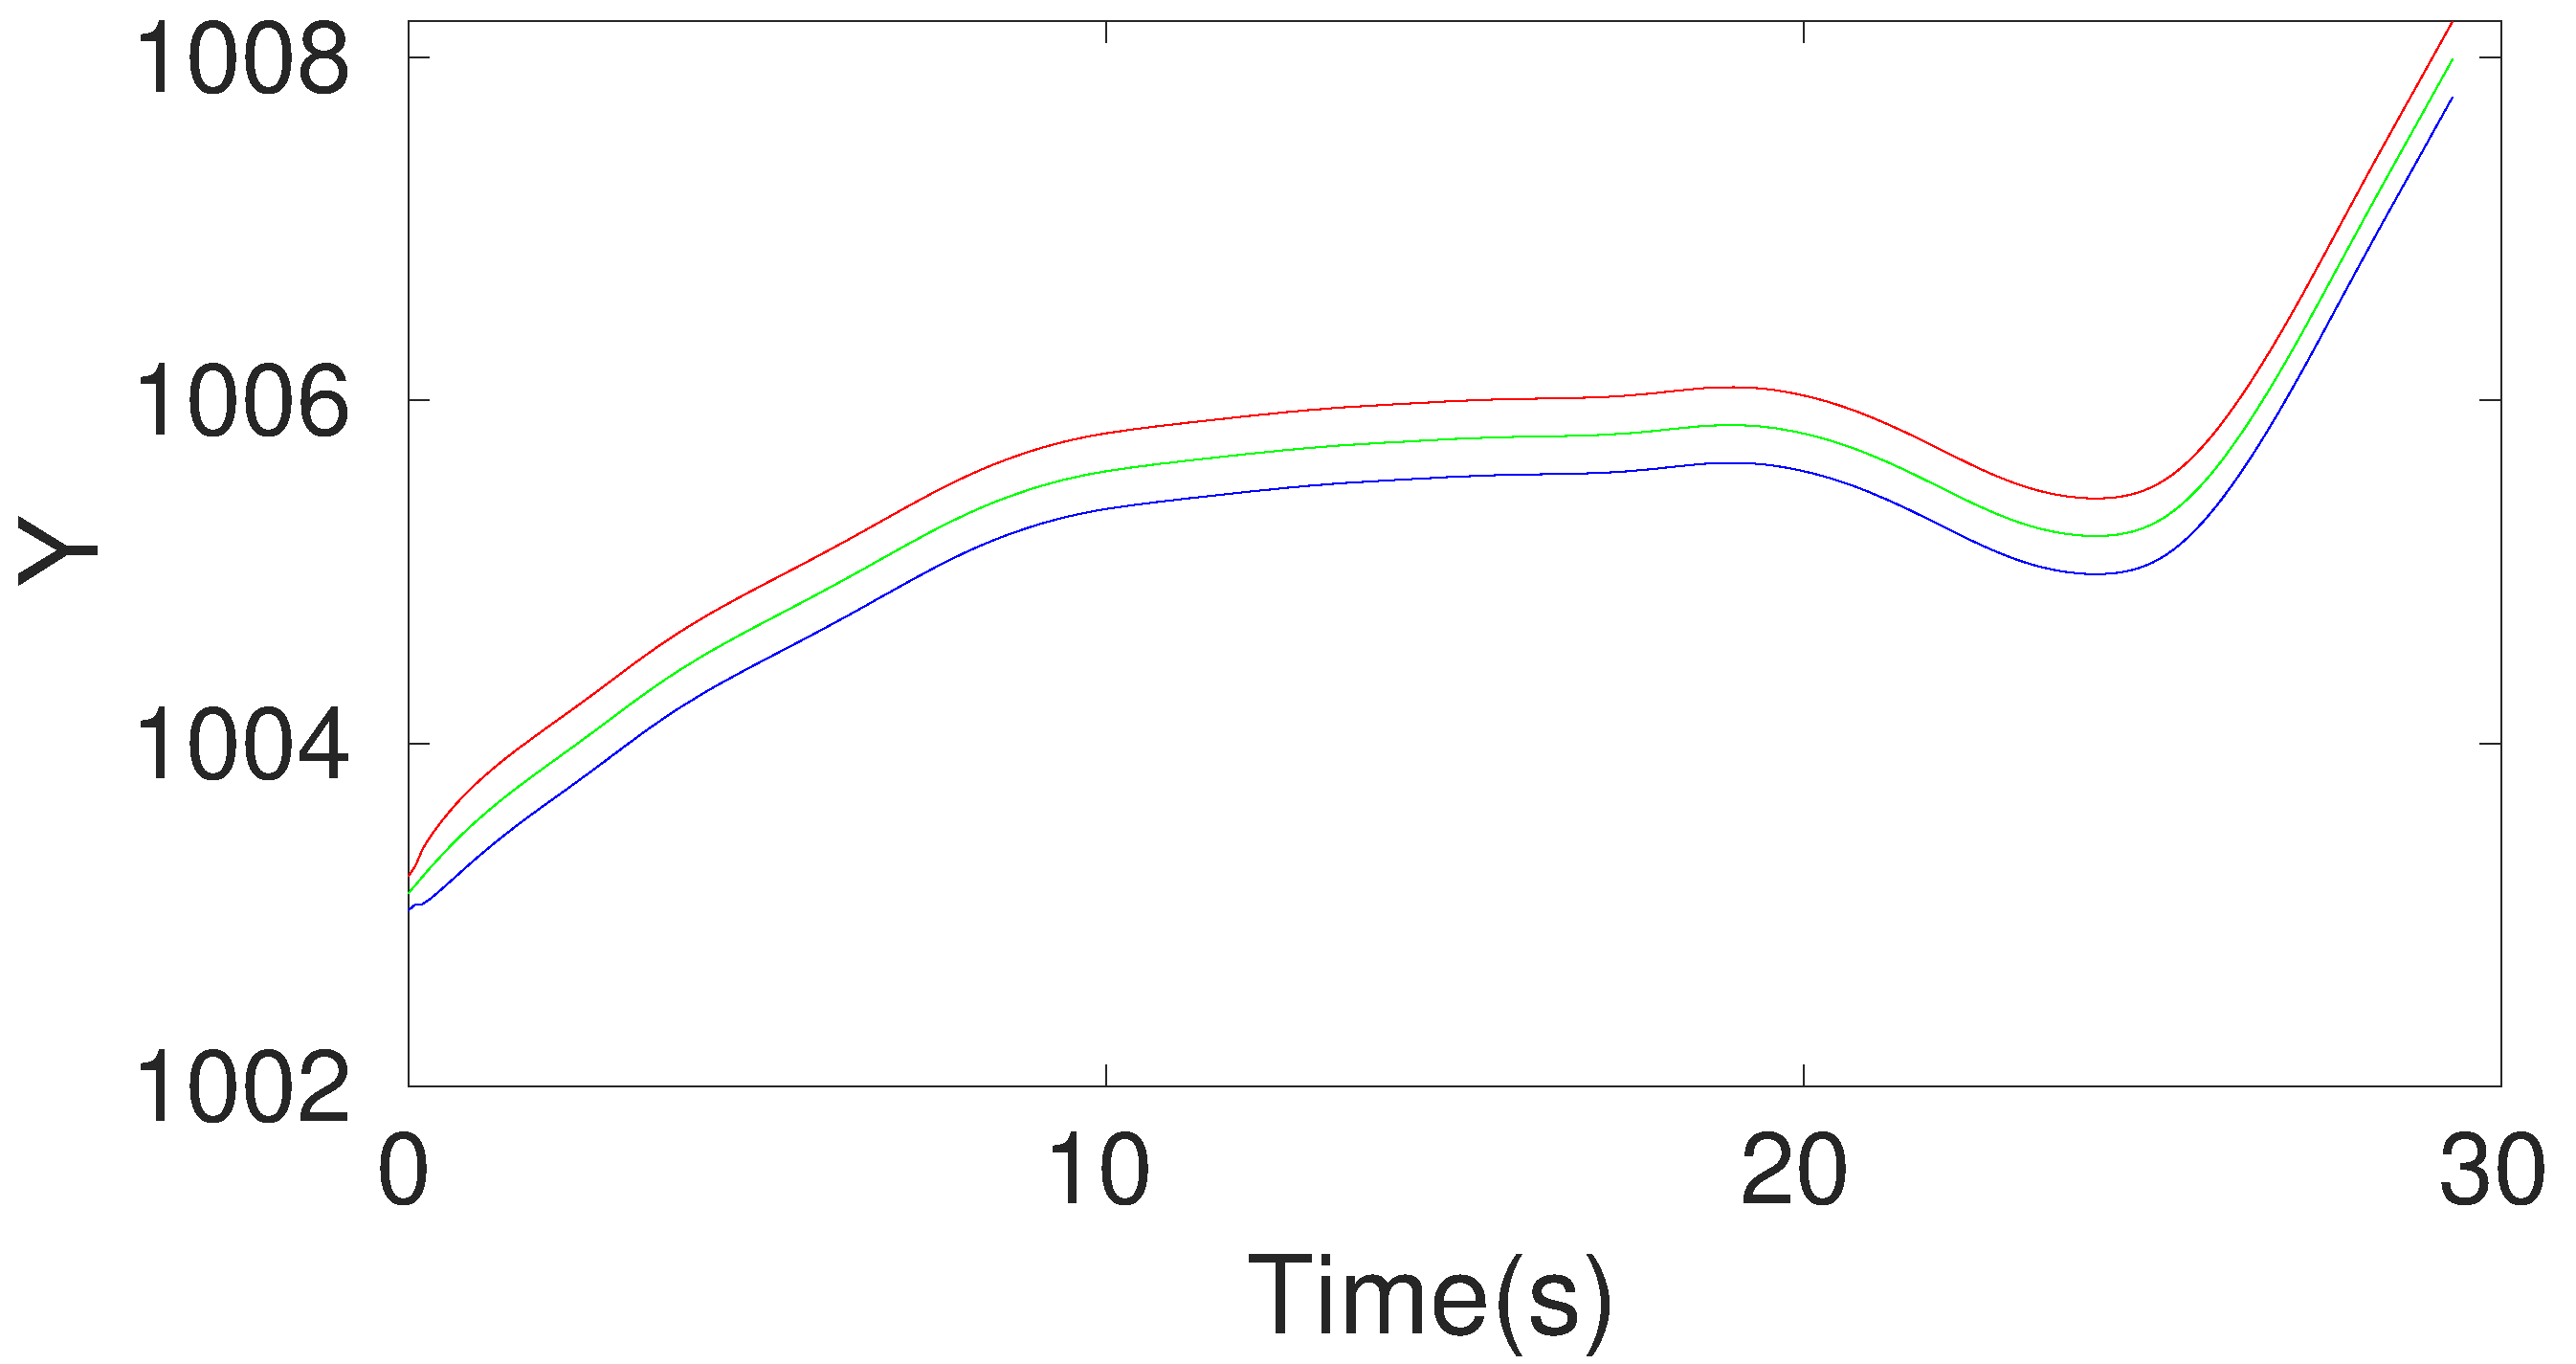
\includegraphics[width=\linewidth]{figures/Frad/s3cvSMY}
\end{subfigure}
\begin{subfigure}{.5\linewidth}
\centering
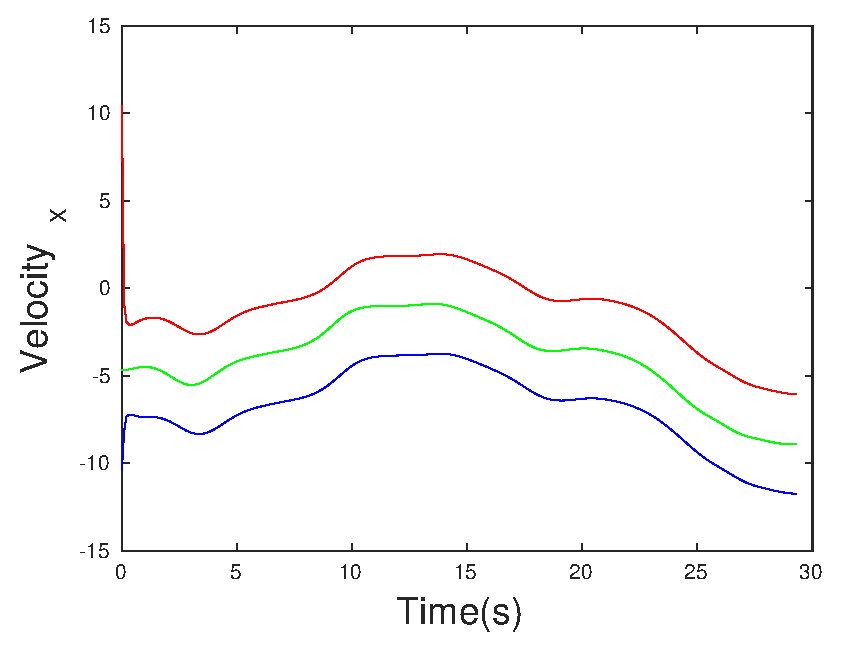
\includegraphics[width=.9\linewidth]{figures/Frad/s3cvSMVelocity_x}
\end{subfigure}
\begin{subfigure}{.5\linewidth}
\centering
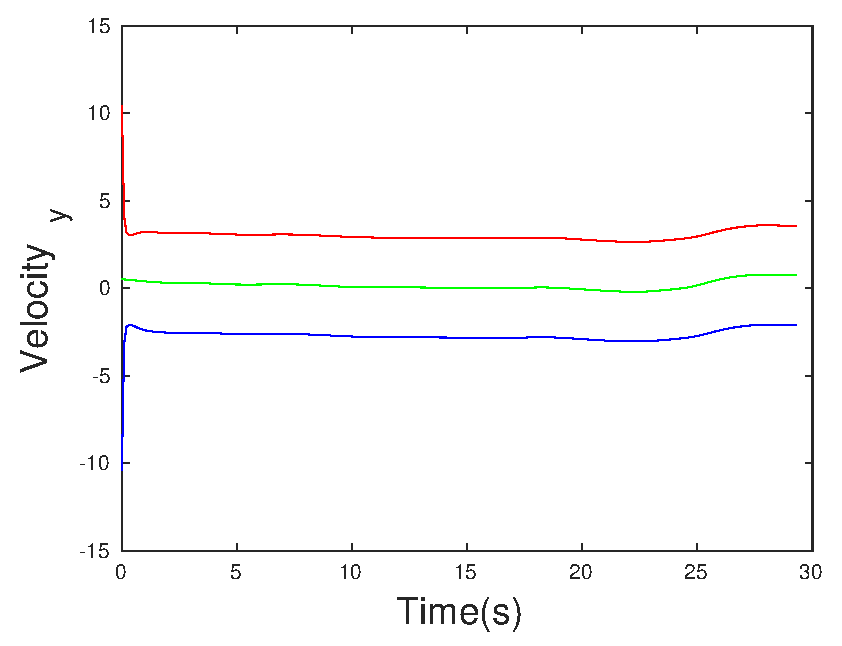
\includegraphics[width=.9\linewidth]{figures/Frad/s3cvSMVelocity_y}
\end{subfigure}
\caption{Estimation using Constant Velocity}
\end{figure}

\begin{figure}[h]
\begin{subfigure}{.5\linewidth}
\centering
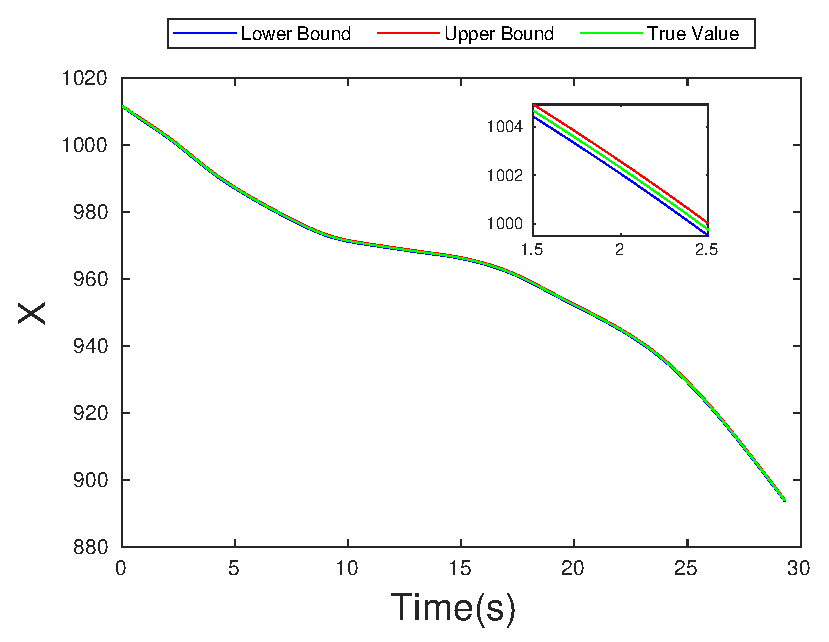
\includegraphics[width=\linewidth]{figures/Frad/s3caSMX}
\end{subfigure}
\begin{subfigure}{.5\linewidth}
\centering
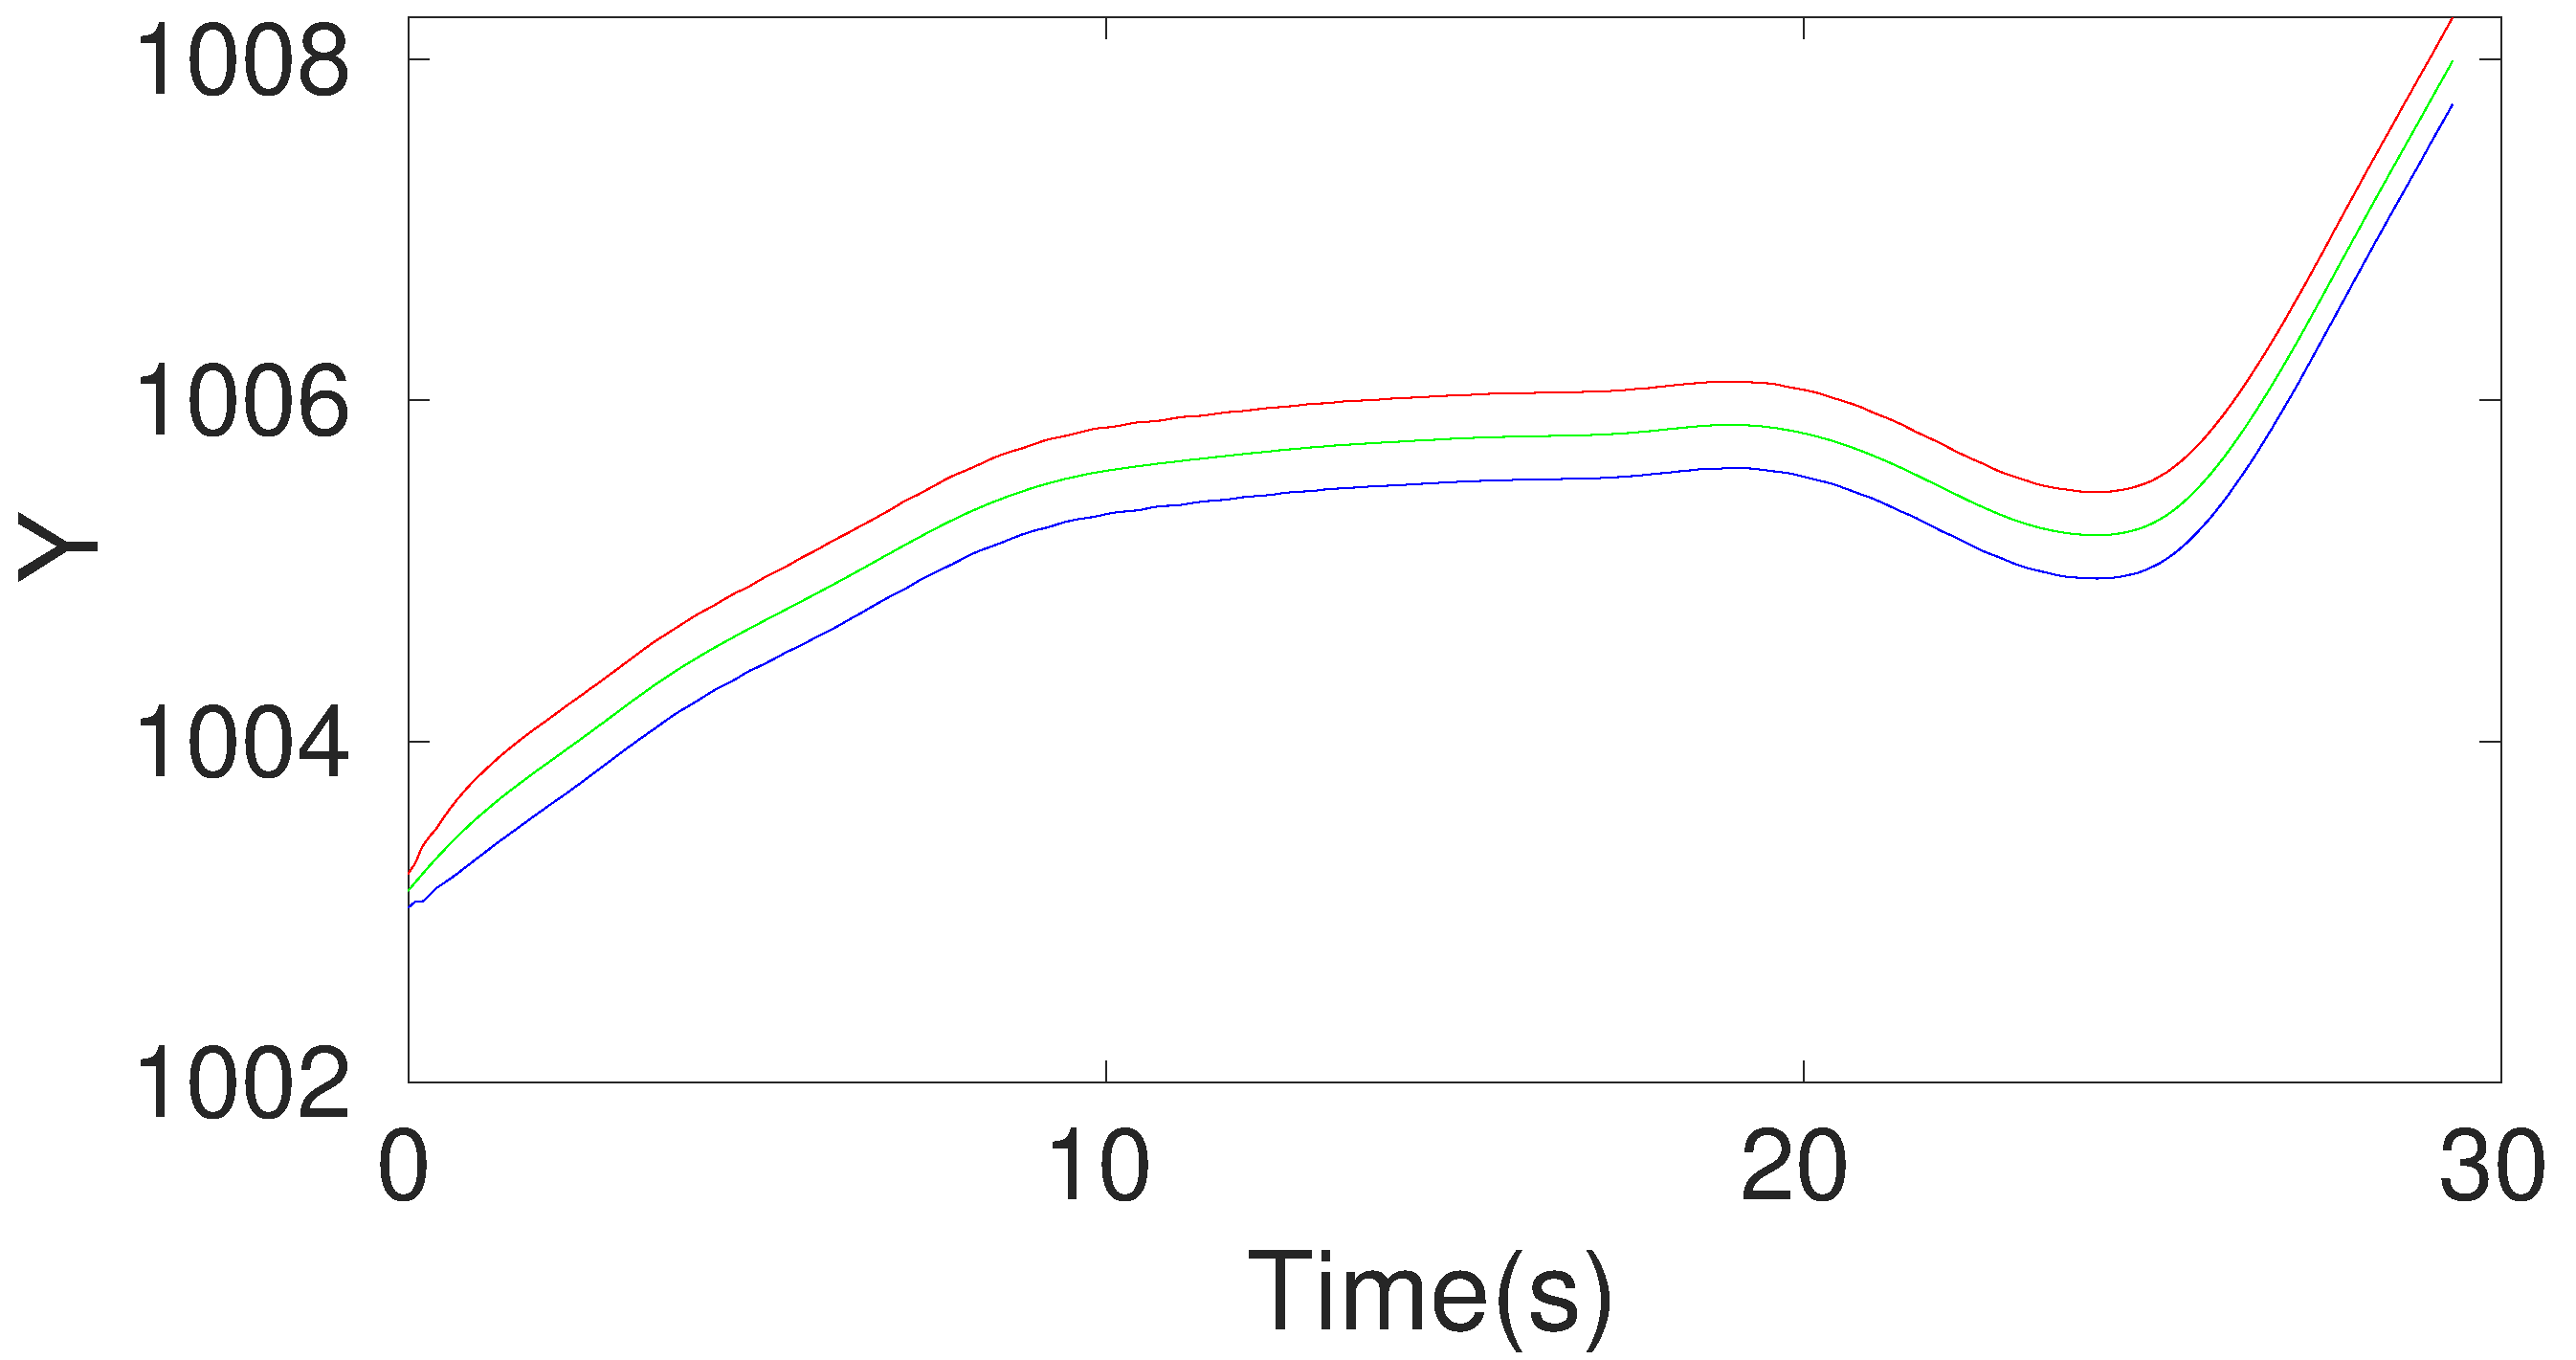
\includegraphics[width=\linewidth]{figures/Frad/s3caSMY}
\end{subfigure}
\begin{subfigure}{.5\linewidth}
\centering
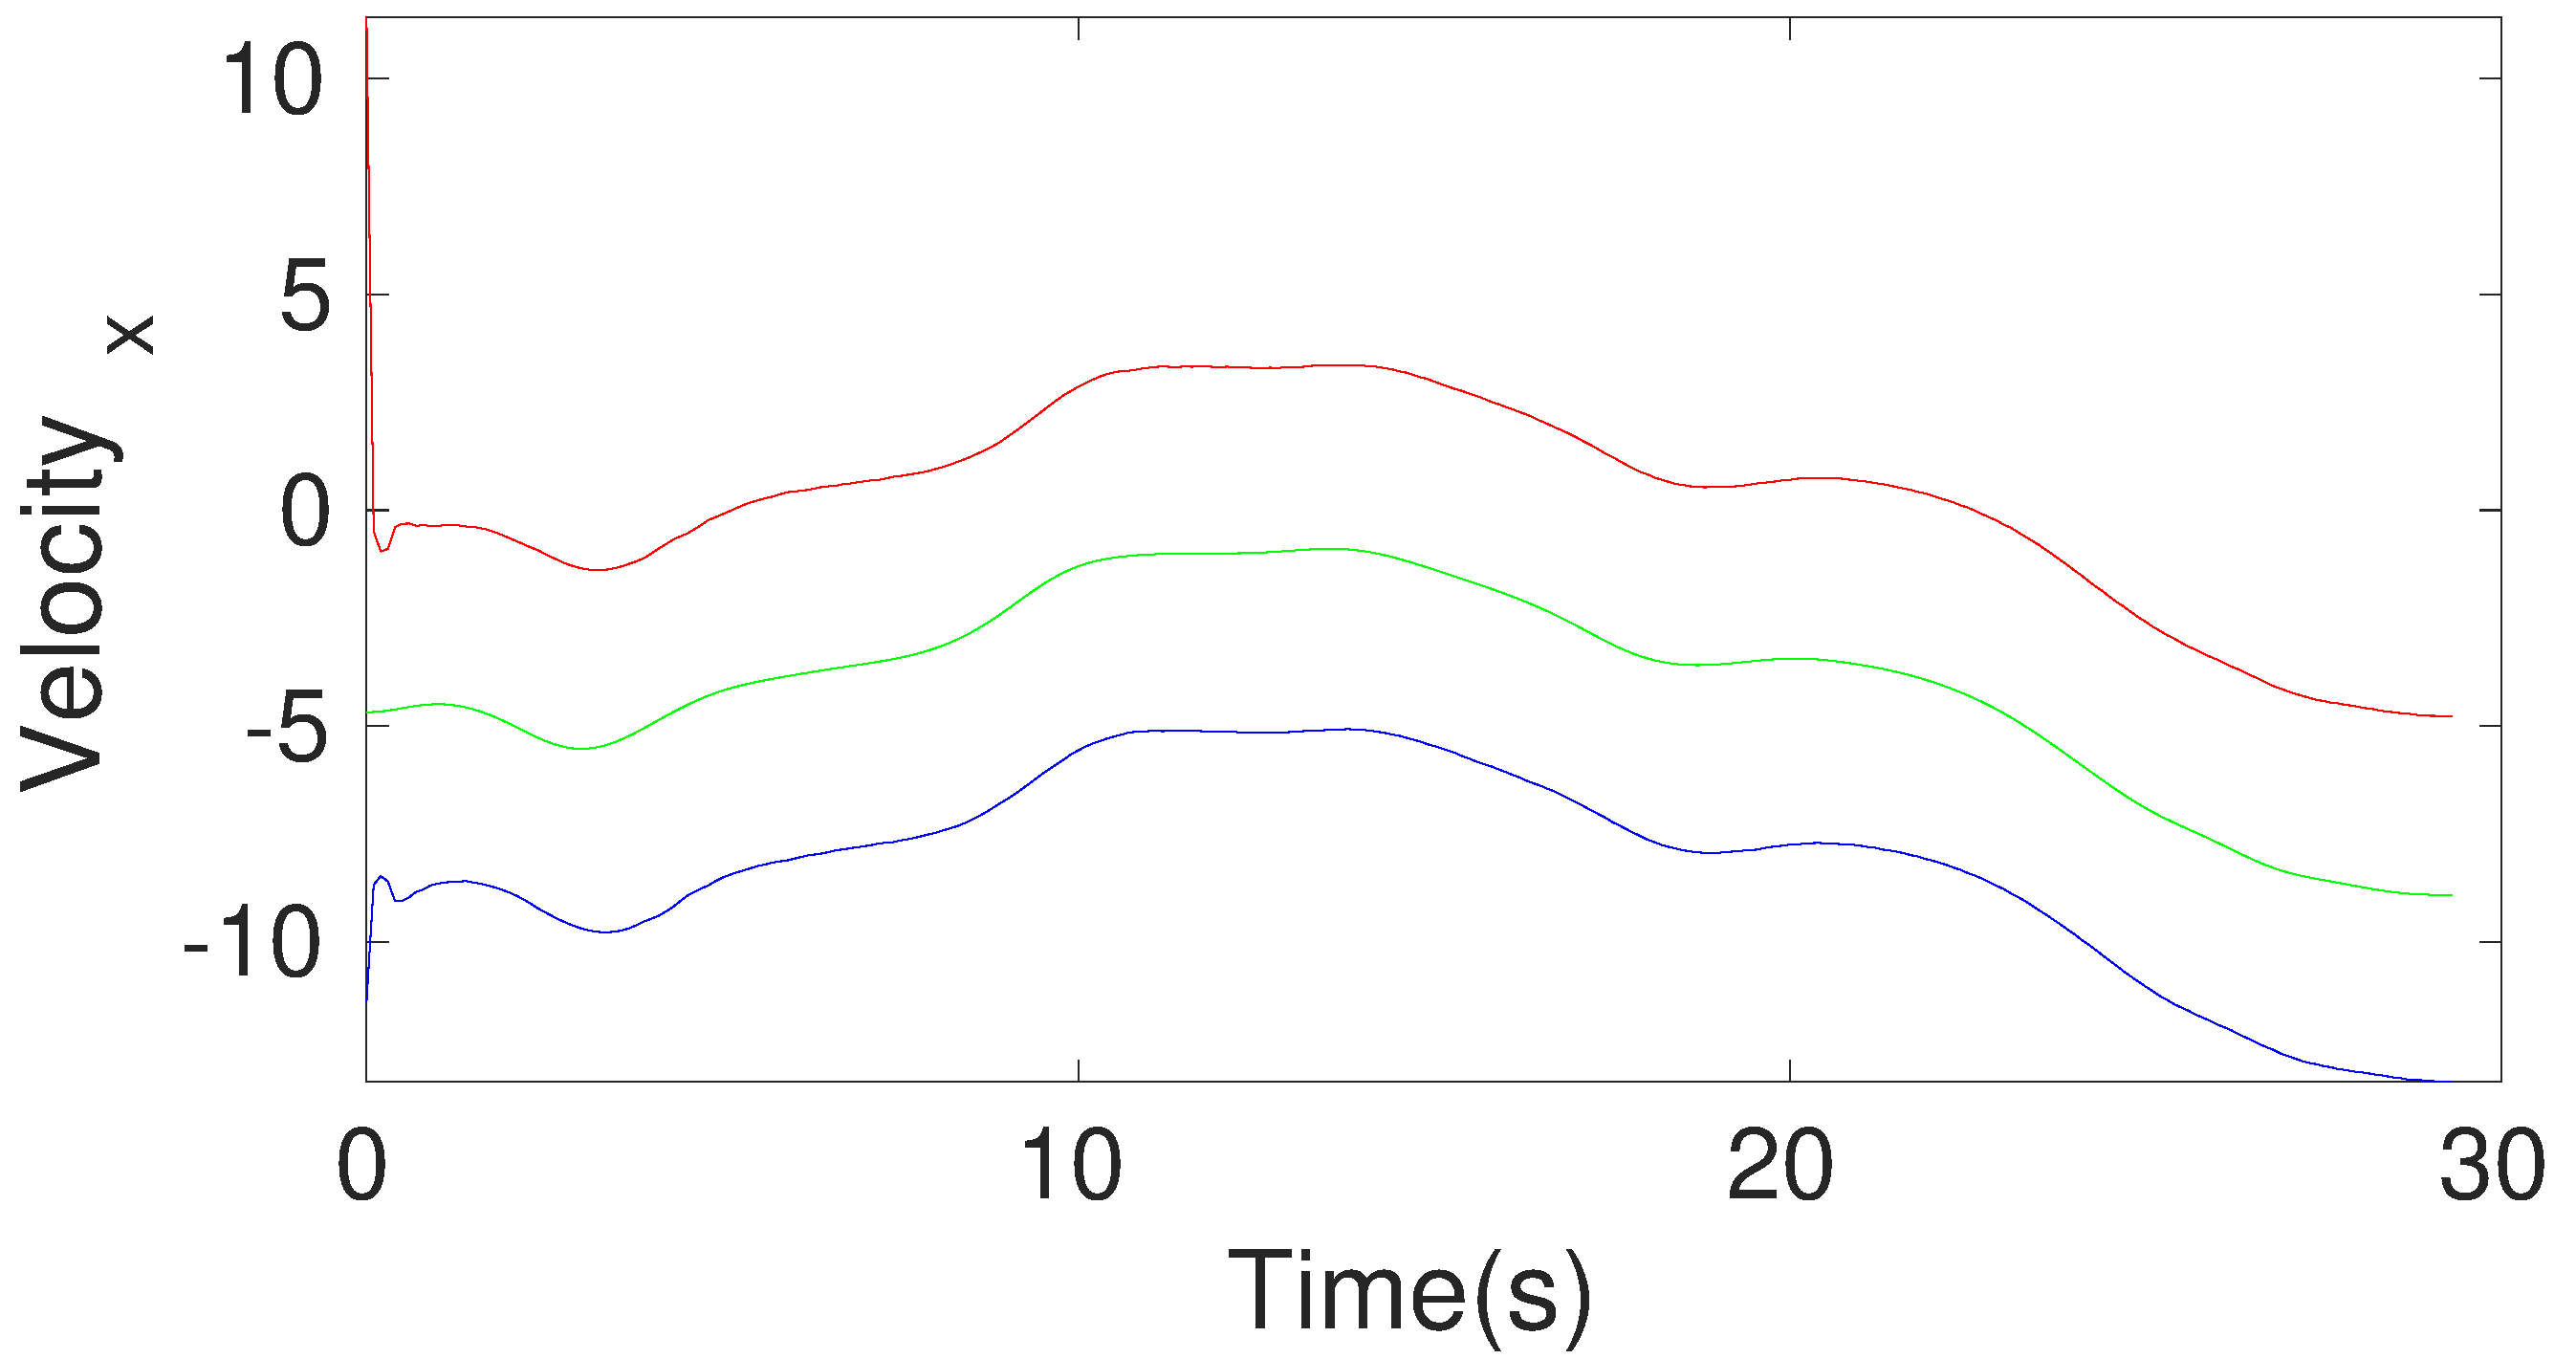
\includegraphics[width=.9\linewidth]{figures/Frad/s3caSMVelocity_x}
\end{subfigure}
\begin{subfigure}{.5\linewidth}
\centering
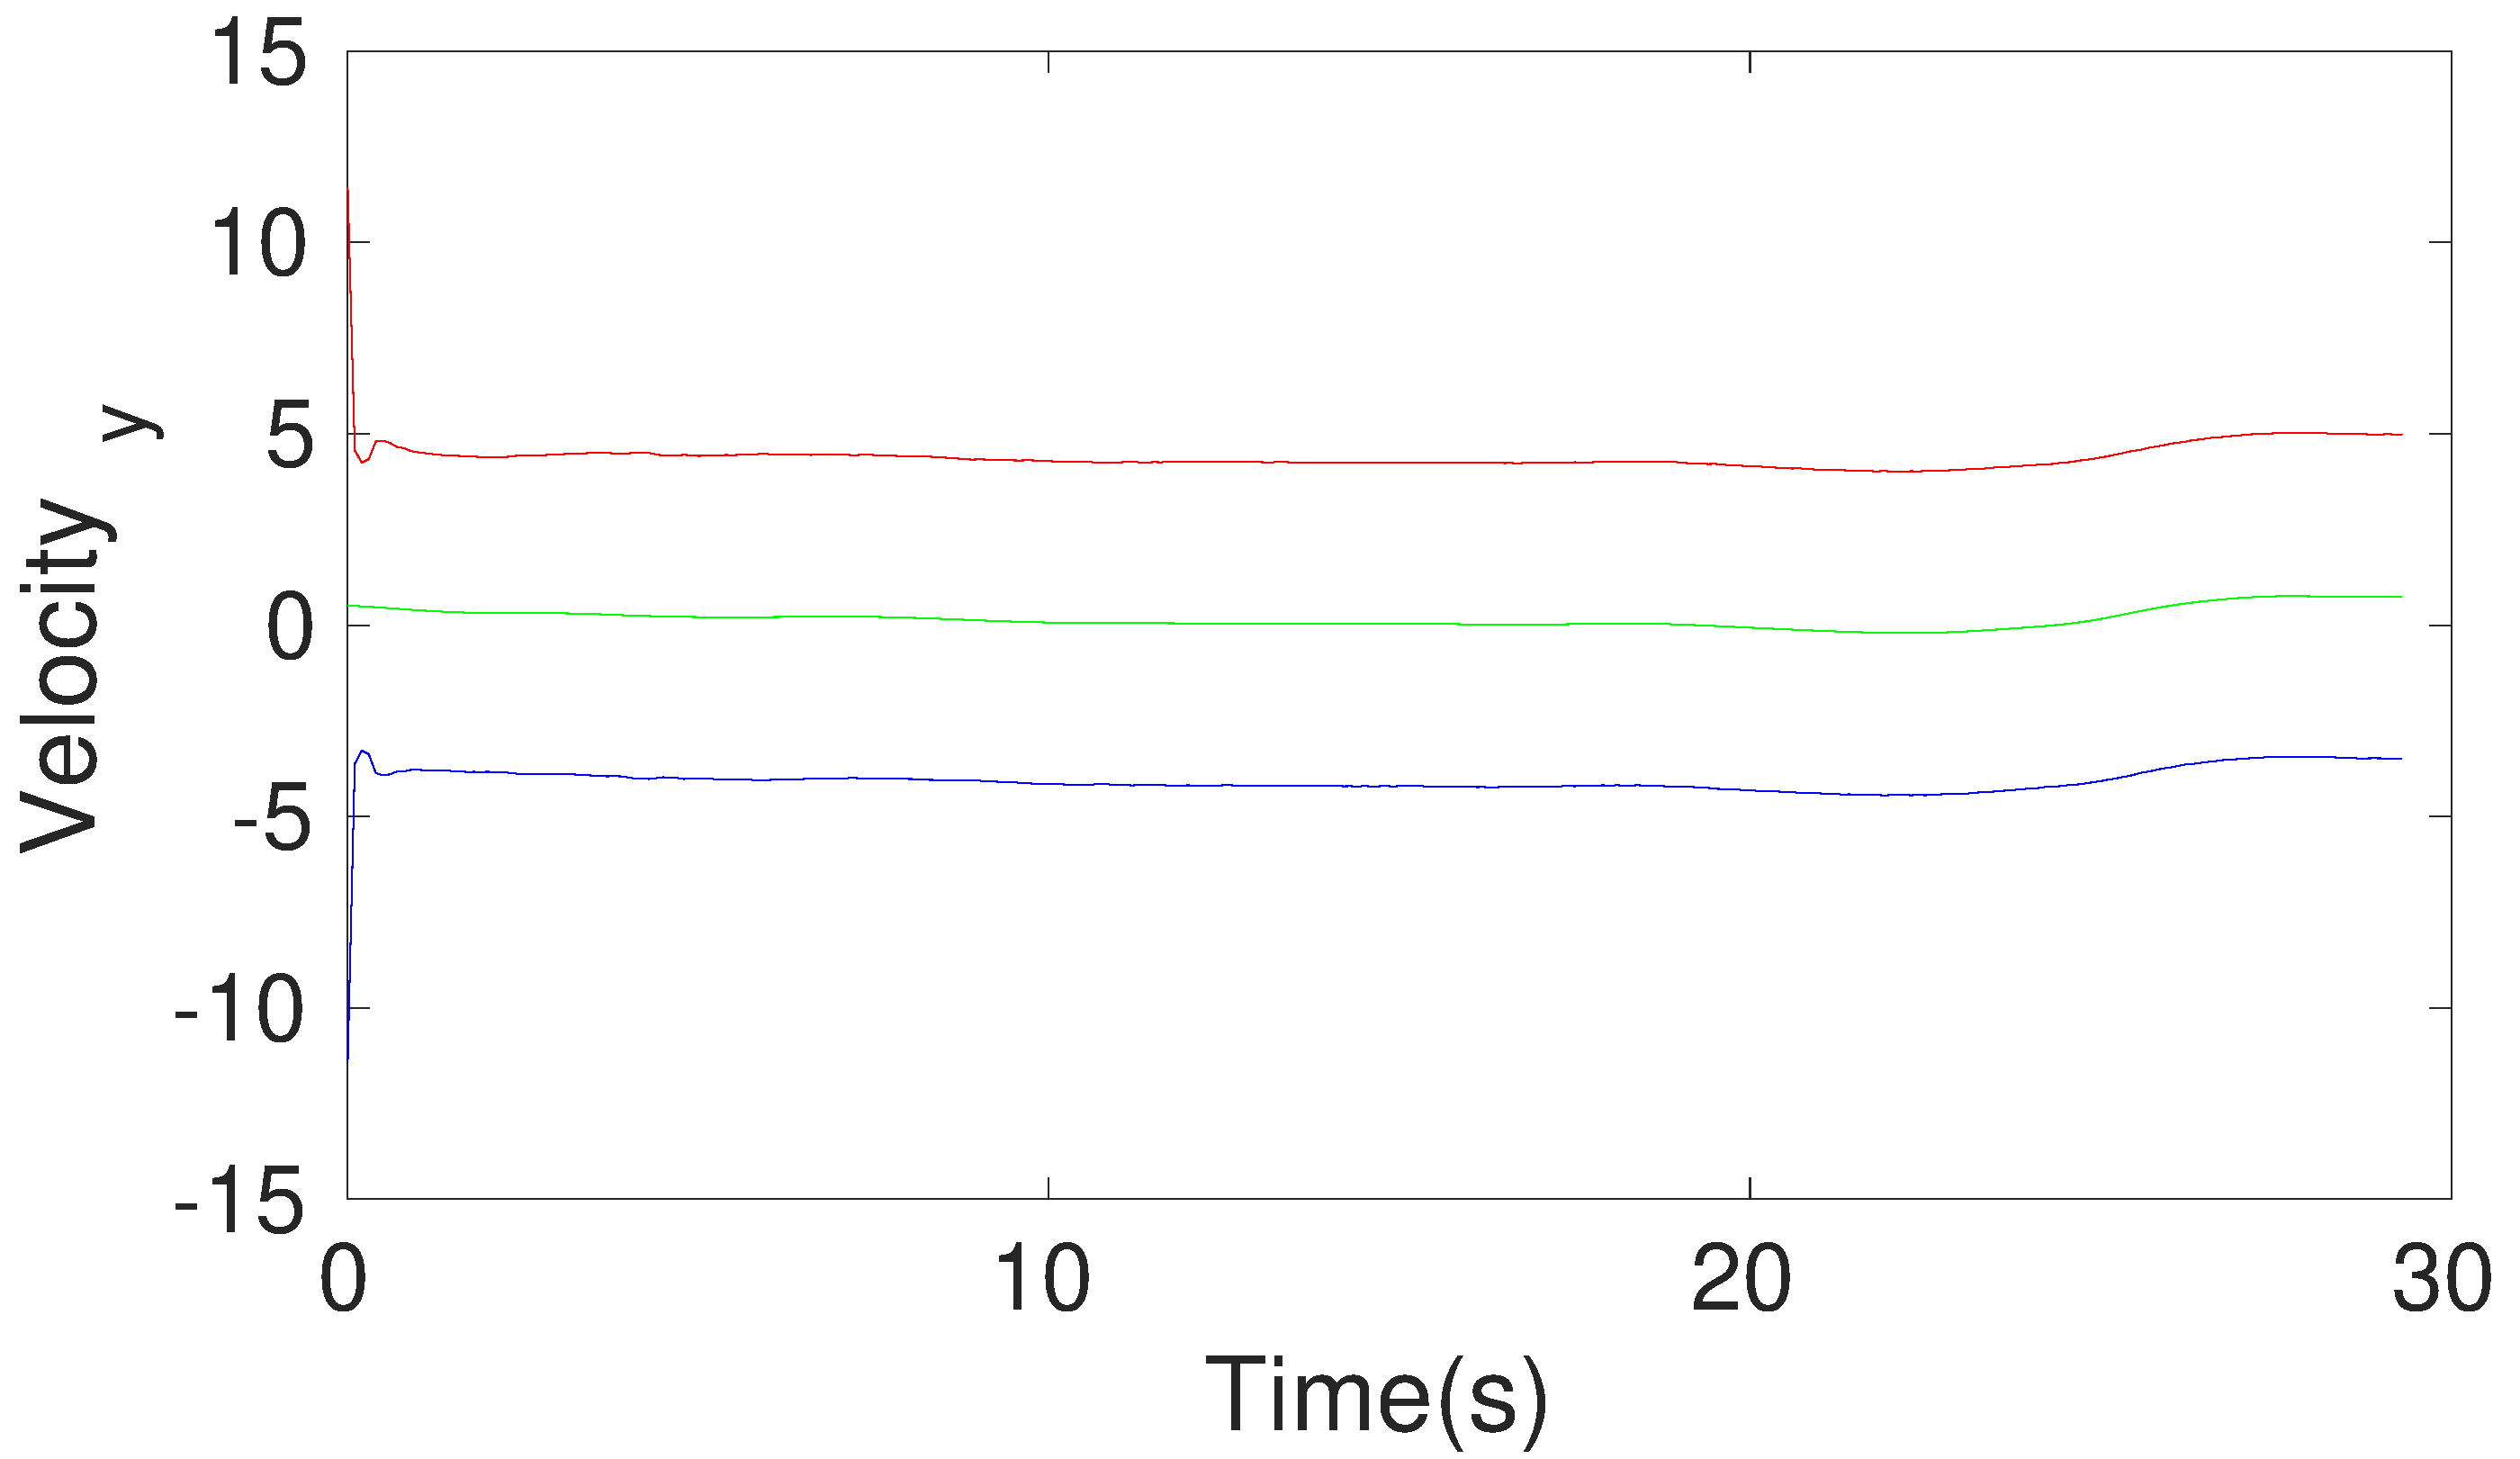
\includegraphics[width=.9\linewidth]{figures/Frad/s3caSMVelocity_y}
\end{subfigure}
\begin{subfigure}{.5\linewidth}
\centering
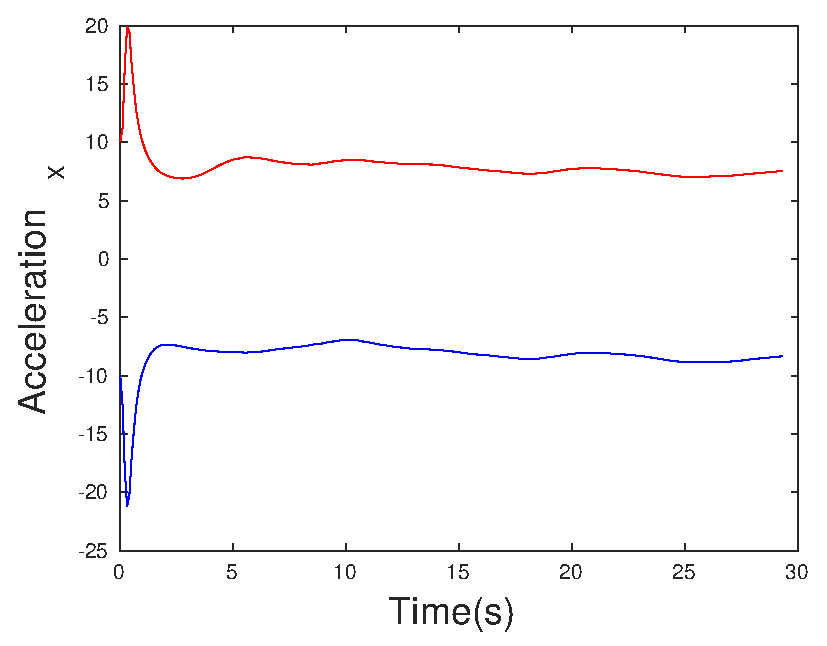
\includegraphics[width=.9\linewidth]{figures/Frad/s3caSMAcceleration_x}
\end{subfigure}
\begin{subfigure}{.5\linewidth}
\centering
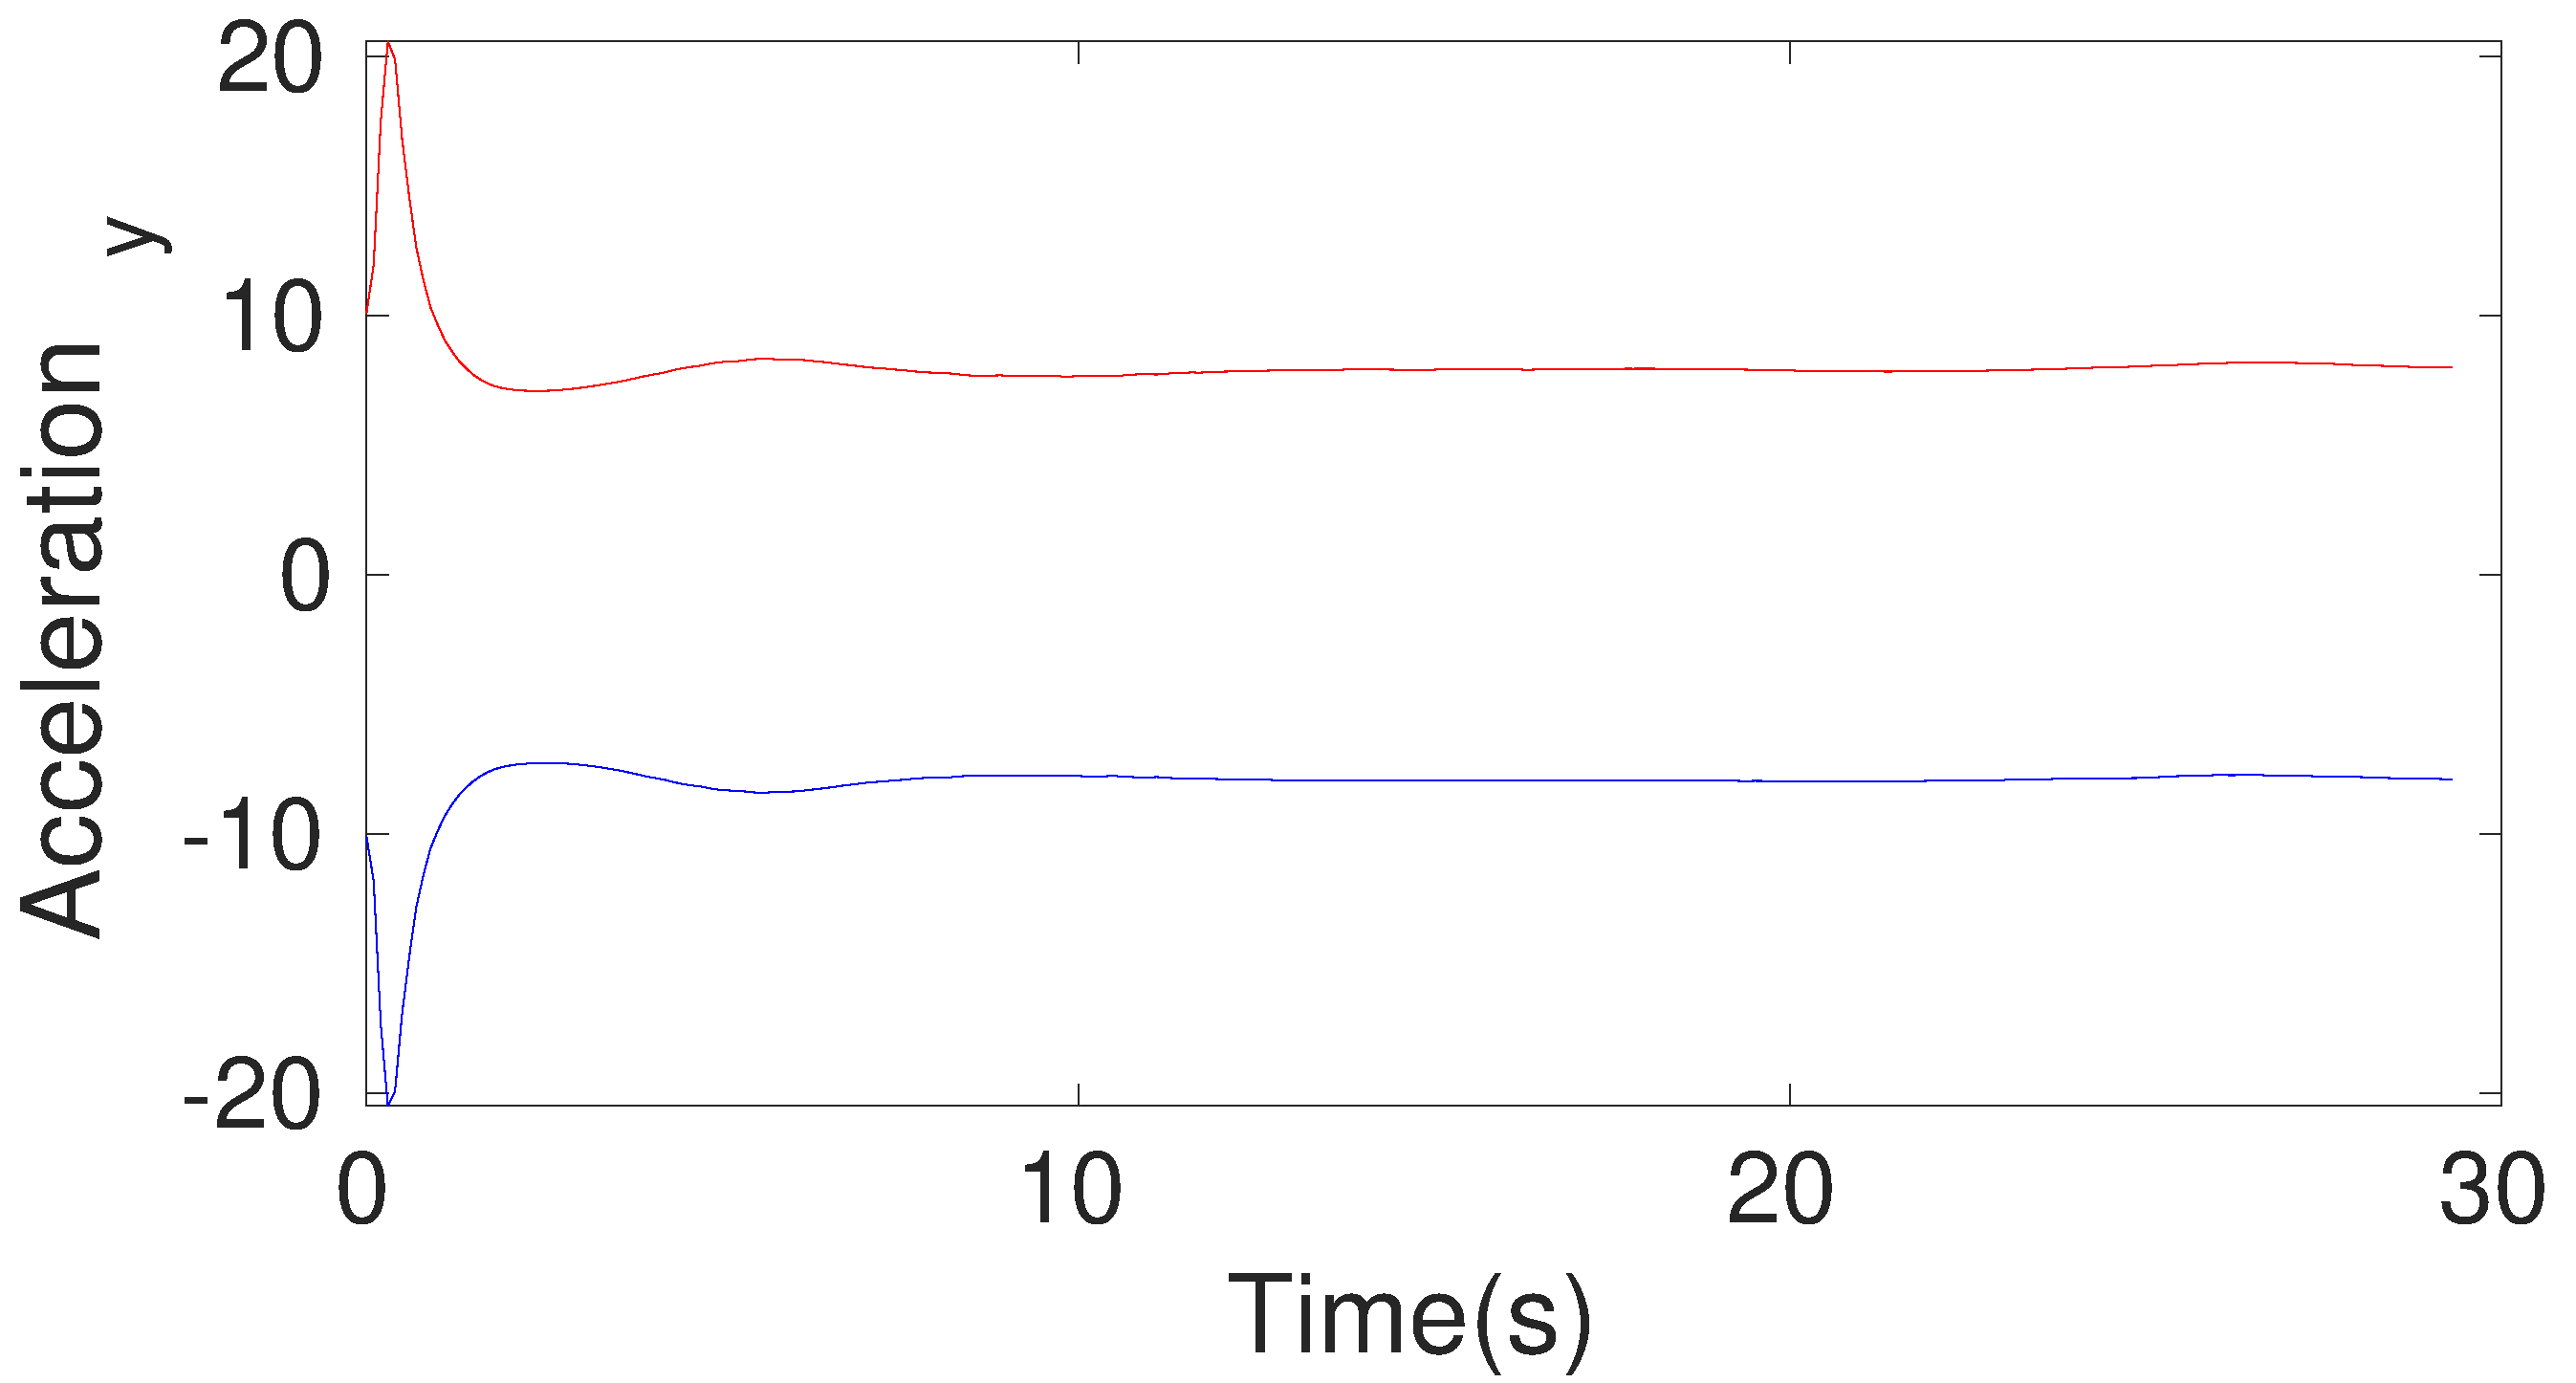
\includegraphics[width=.9\linewidth]{figures/Frad/s3caSMAcceleration_y}
\end{subfigure}
\caption{Estimation using Constant Acceleration}
\end{figure}

\begin{figure}[h]
\begin{subfigure}{.5\linewidth}
\centering
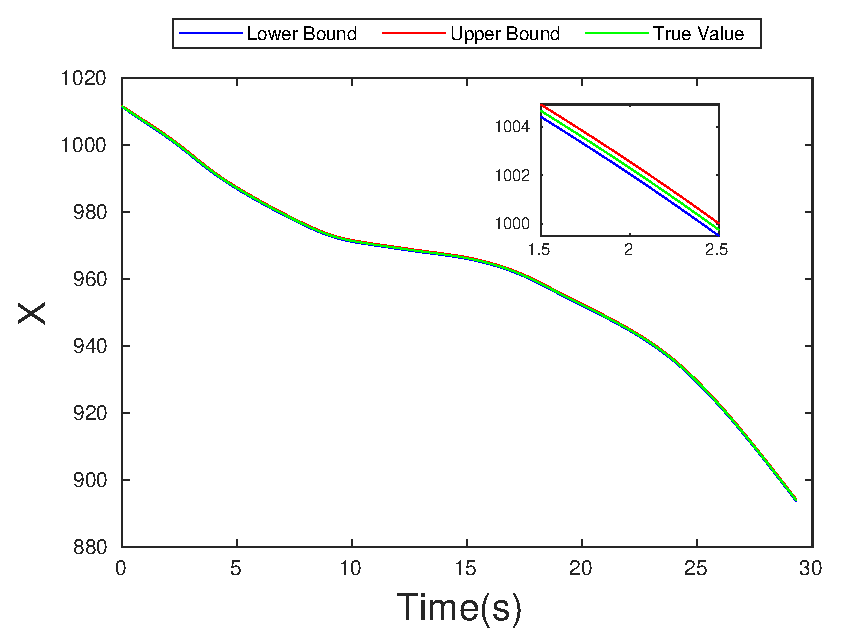
\includegraphics[width=\linewidth]{figures/Frad/s3pmSMX}
\end{subfigure}
\begin{subfigure}{.5\linewidth}
\centering
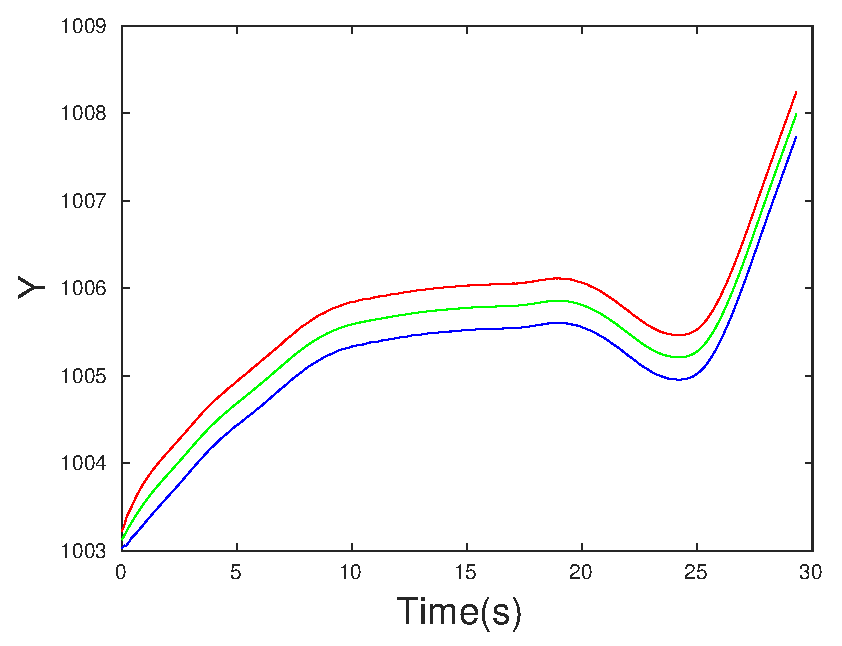
\includegraphics[width=\linewidth]{figures/Frad/s3pmSMY}
\end{subfigure}
\begin{subfigure}{.5\linewidth}
\centering
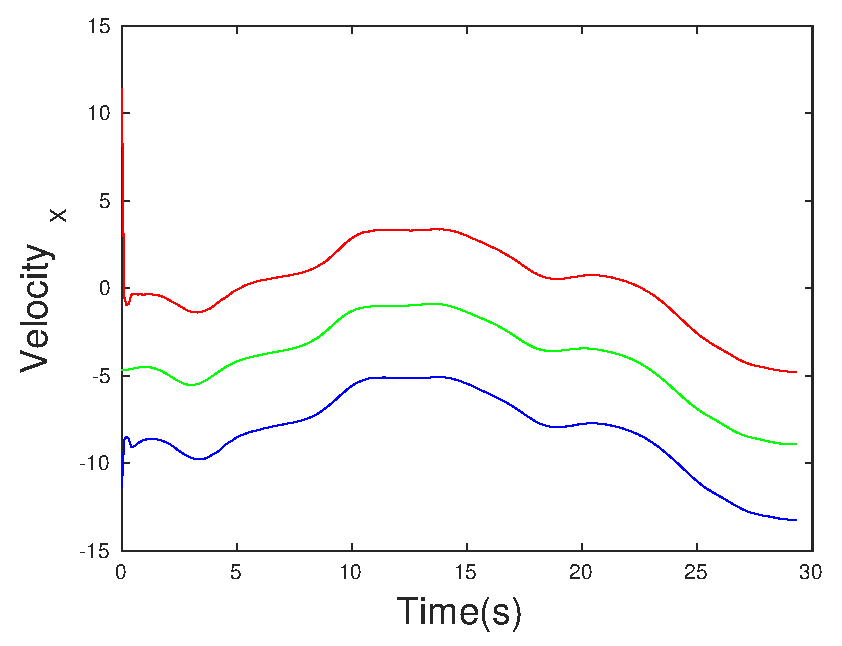
\includegraphics[width=.9\linewidth]{figures/Frad/s3pmSMVelocity_x}
\end{subfigure}
\begin{subfigure}{.5\linewidth}
\centering
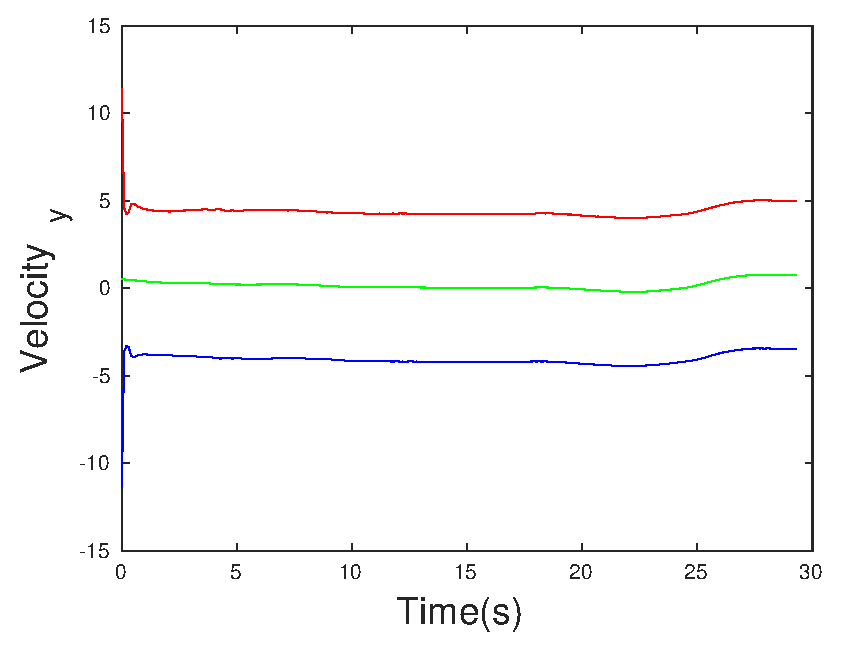
\includegraphics[width=.9\linewidth]{figures/Frad/s3pmSMVelocity_y}
\end{subfigure}
\begin{subfigure}{.5\linewidth}
\centering
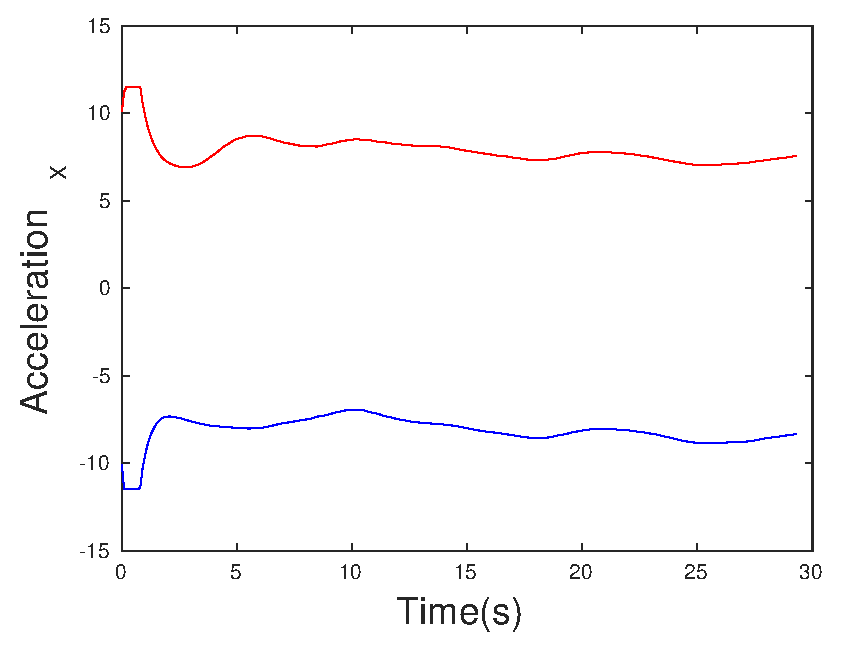
\includegraphics[width=.9\linewidth]{figures/Frad/s3pmSMAcceleration_x}
\end{subfigure}
\begin{subfigure}{.5\linewidth}
\centering
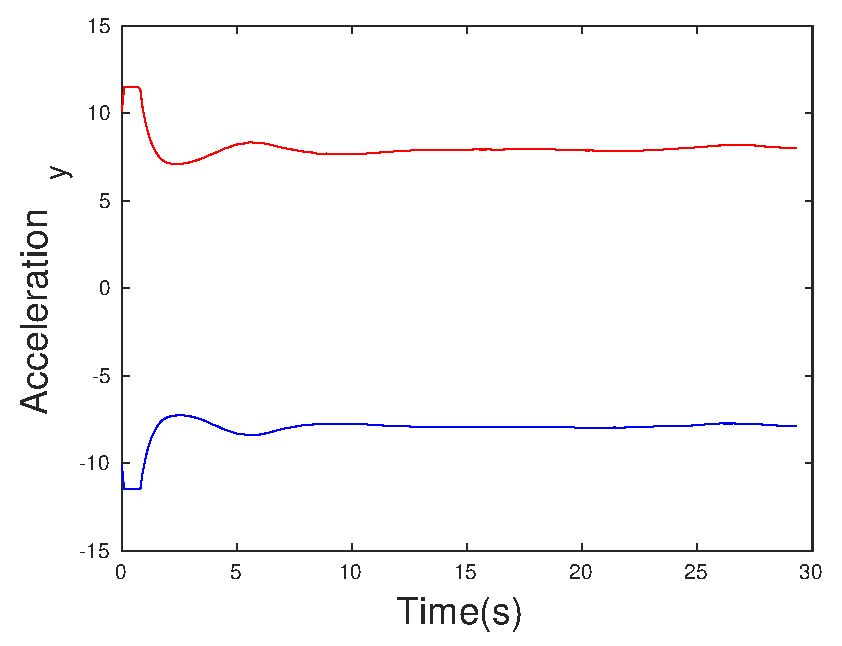
\includegraphics[width=.9\linewidth]{figures/Frad/s3pmSMAcceleration_y}
\end{subfigure}
\caption{Estimation using Point Mass Model}
\end{figure}

\clearpage
\subsection{Segment Minimization using P-Radius}
\FloatBarrier
\begin{figure}[h]
\begin{subfigure}{.5\linewidth}
\centering
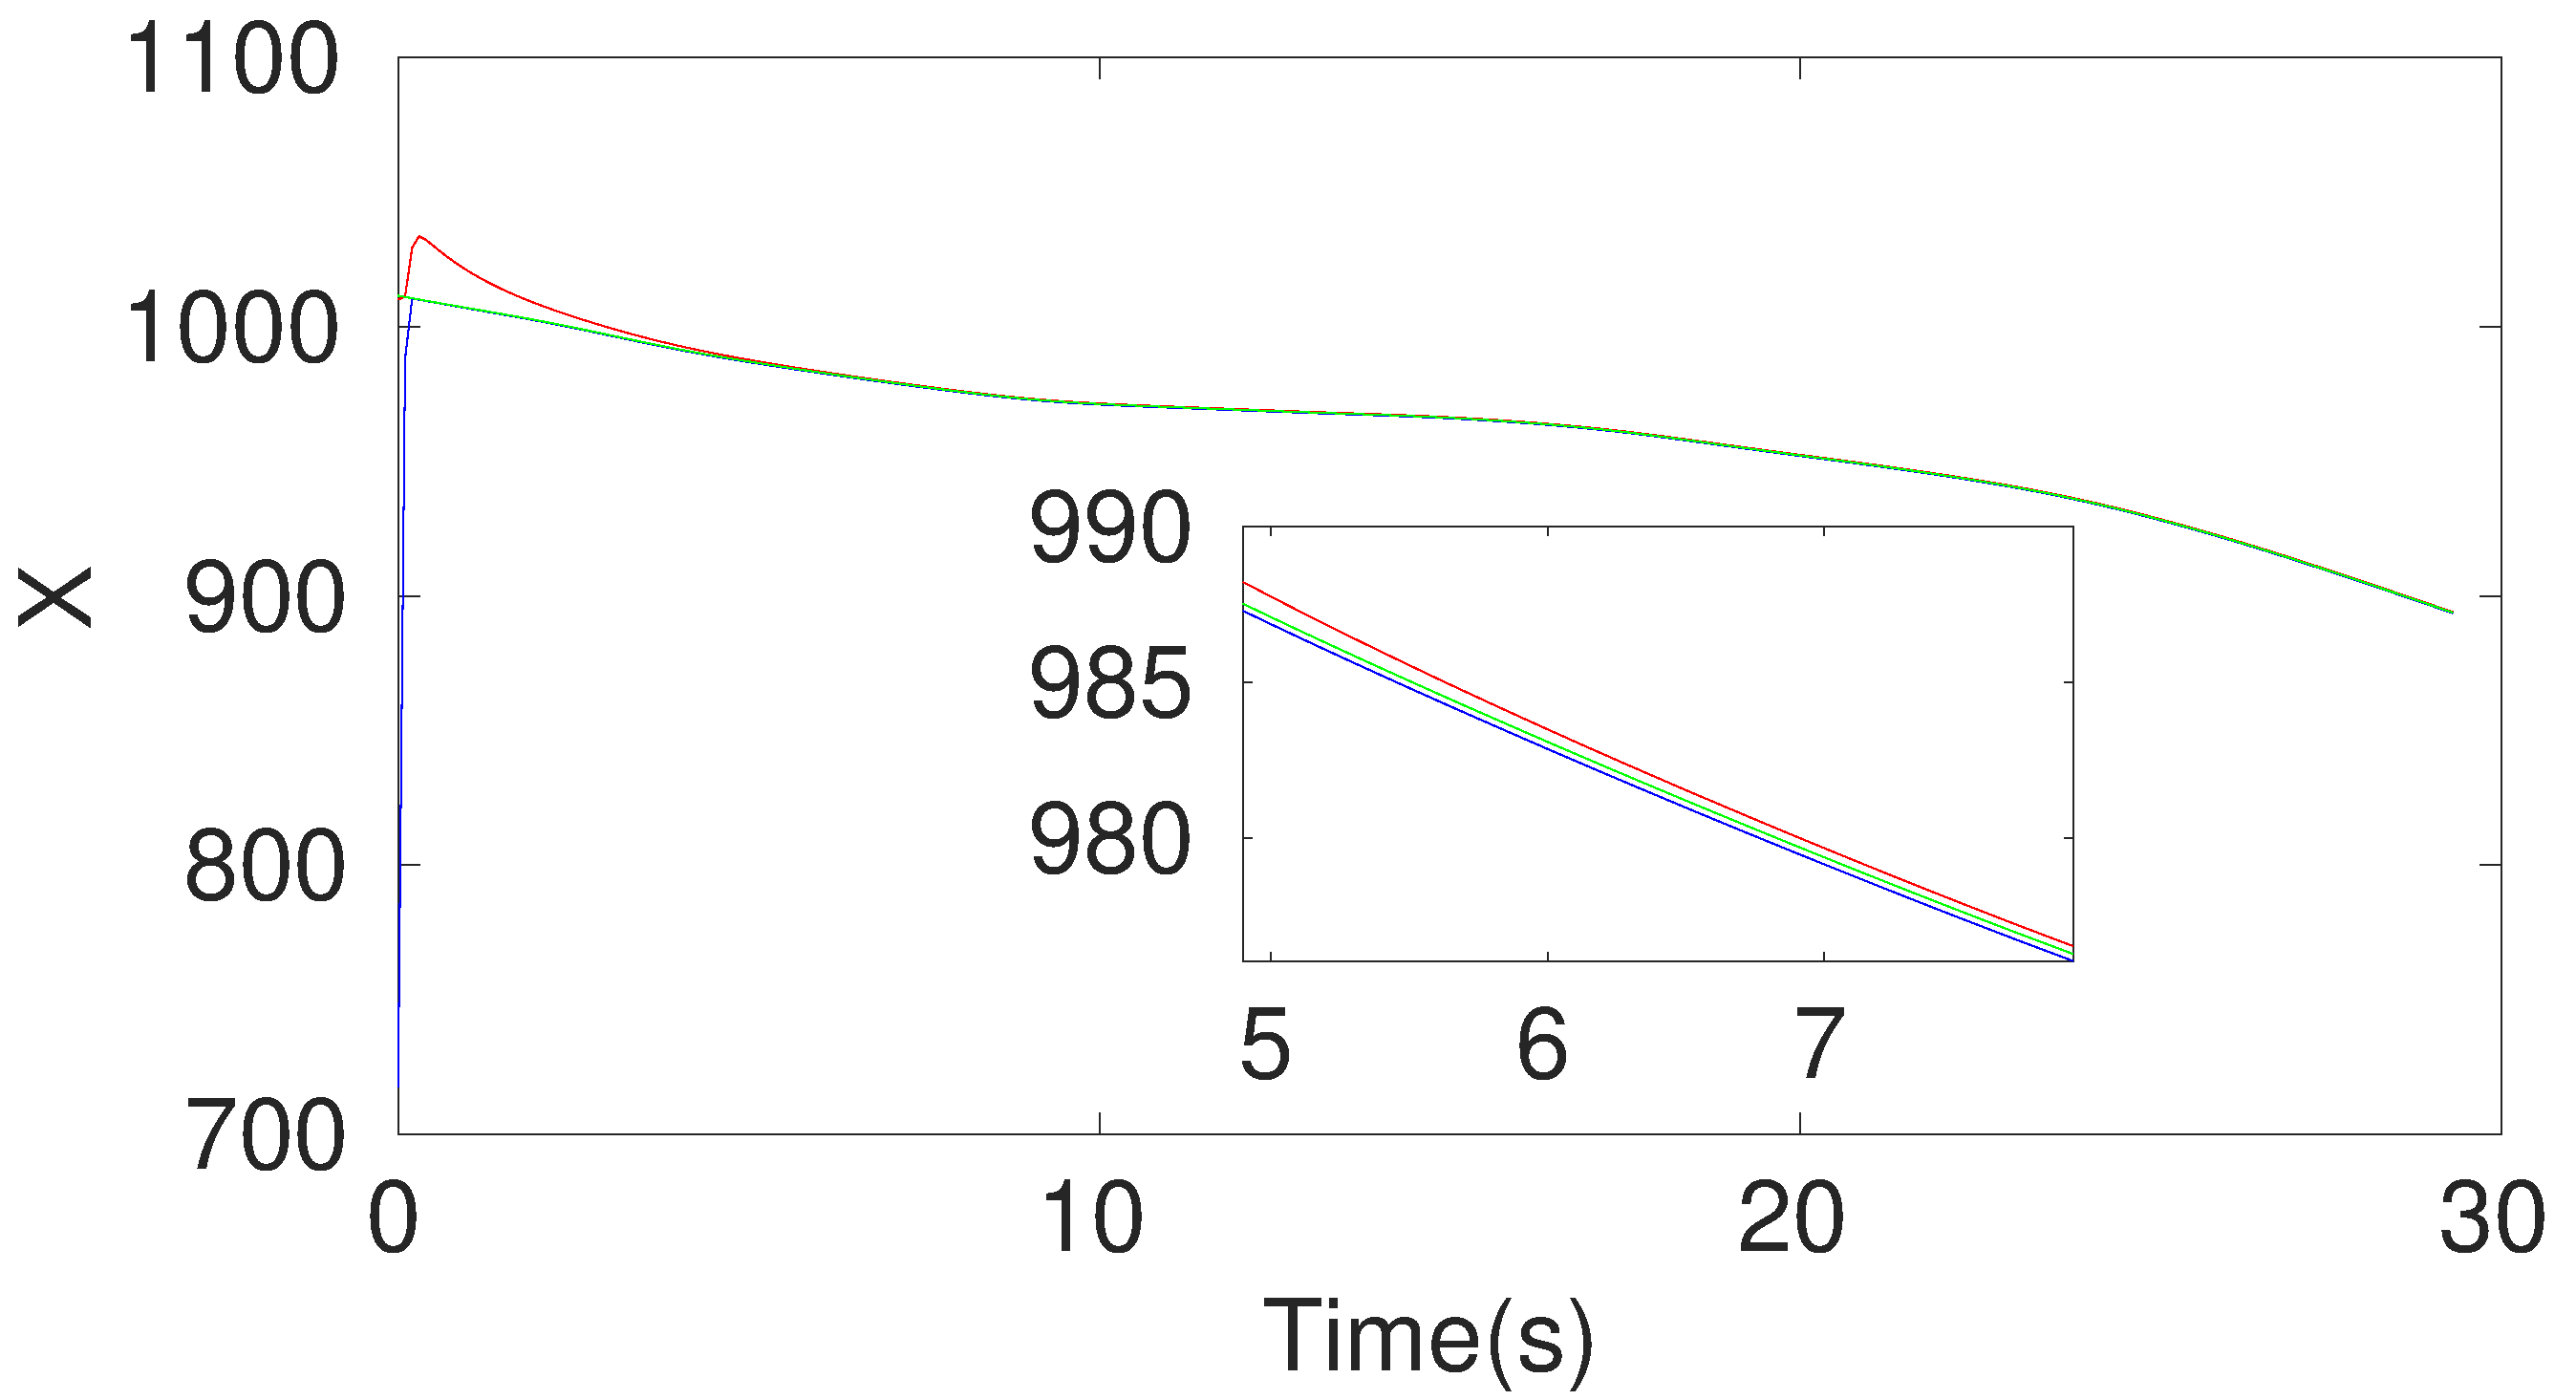
\includegraphics[width=\linewidth]{figures/Prad/s3cvpradX}
\end{subfigure}
\begin{subfigure}{.5\linewidth}
\centering
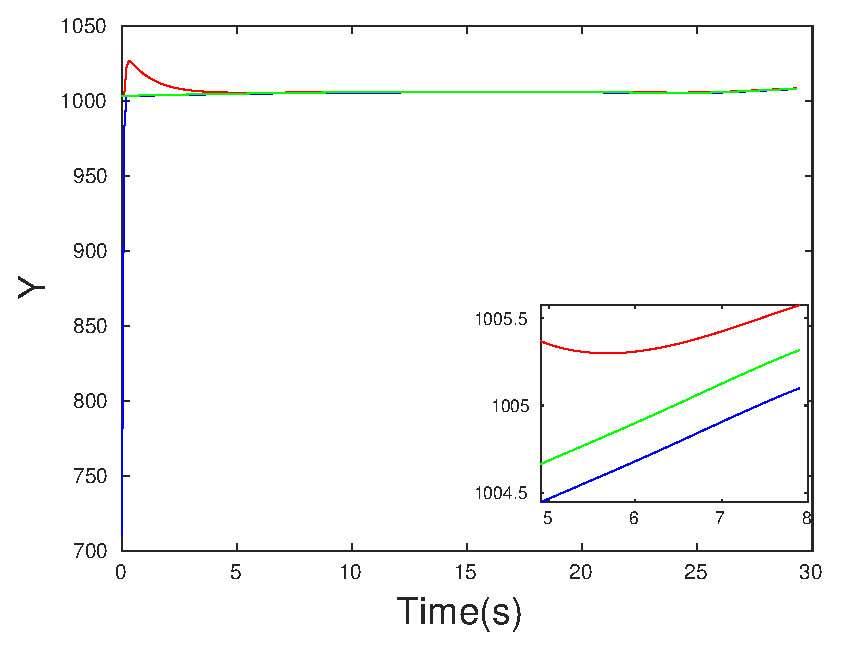
\includegraphics[width=\linewidth]{figures/Prad/s3cvpradY}
\end{subfigure}
\begin{subfigure}{.5\linewidth}
\centering
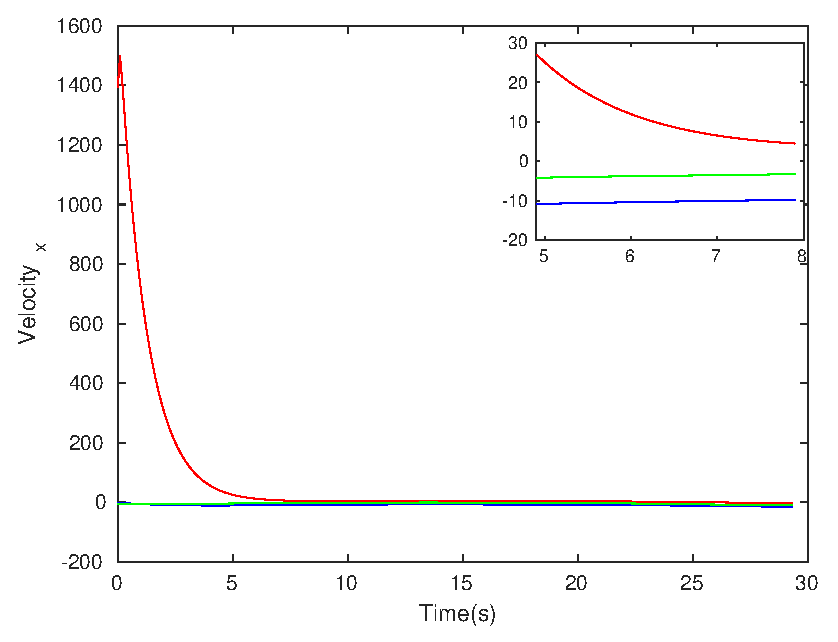
\includegraphics[width=.9\linewidth]{figures/Prad/s3cvpradVelocity_x}
\end{subfigure}
\begin{subfigure}{.5\linewidth}
\centering
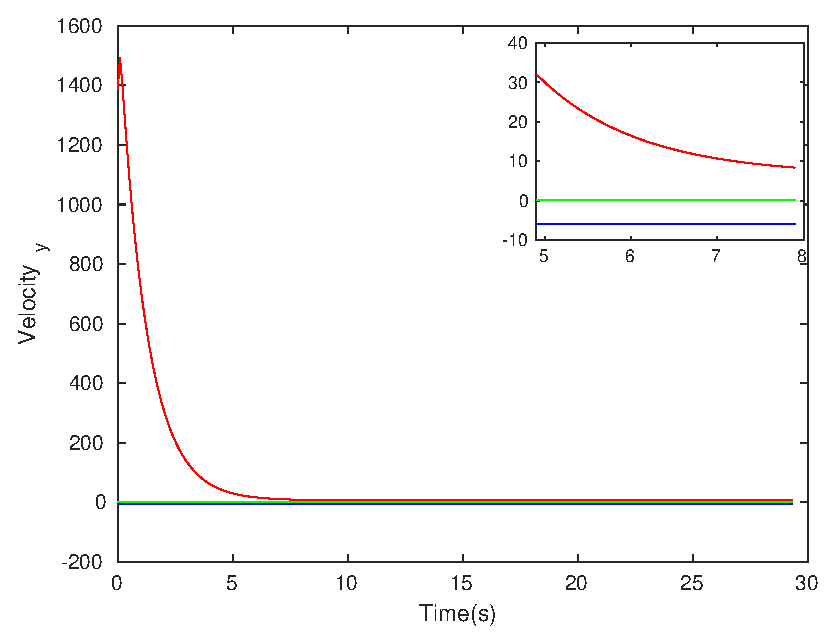
\includegraphics[width=.9\linewidth]{figures/Prad/s3cvpradVelocity_y}
\end{subfigure}
\caption{Estimation using Constant Velocity}
\end{figure}

\begin{figure}[h]
\begin{subfigure}{.5\linewidth}
\centering
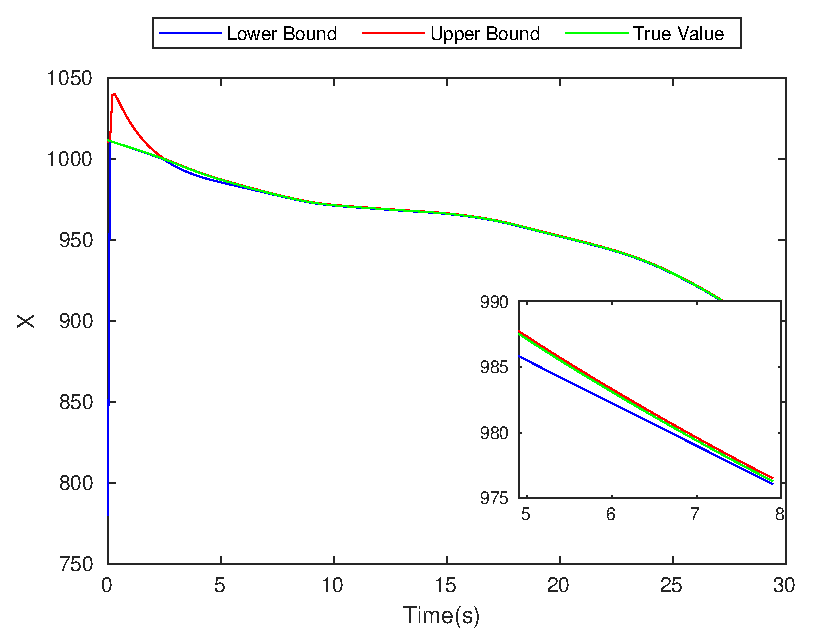
\includegraphics[width=\linewidth]{figures/Prad/s3capradX}
\end{subfigure}
\begin{subfigure}{.5\linewidth}
\centering
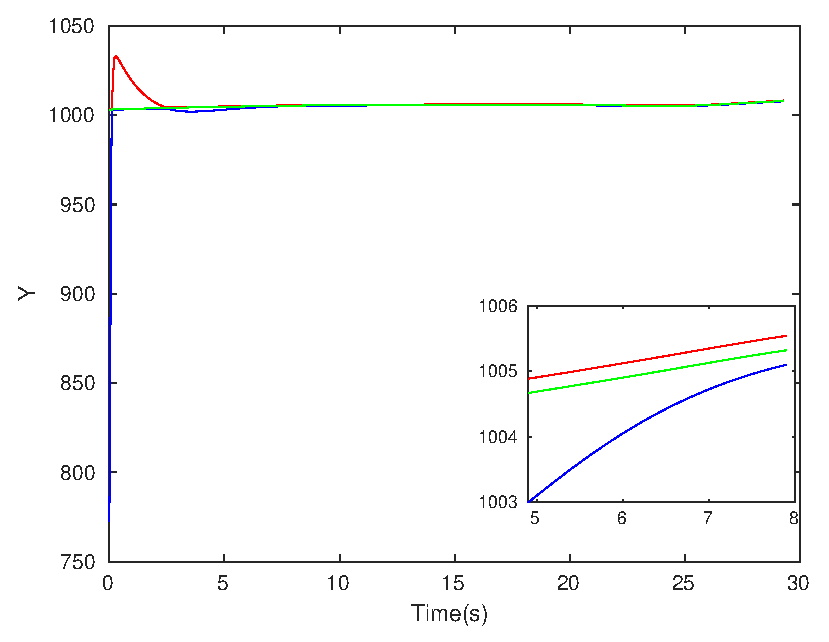
\includegraphics[width=\linewidth]{figures/Prad/s3capradY}
\end{subfigure}
\begin{subfigure}{.5\linewidth}
\centering
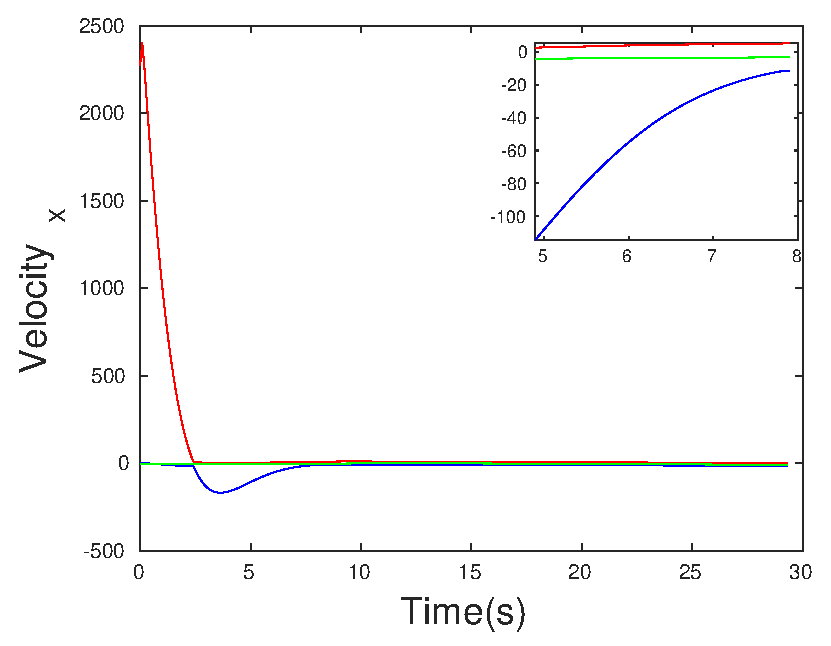
\includegraphics[width=.9\linewidth]{figures/Prad/s3capradVelocity_x}
\end{subfigure}
\begin{subfigure}{.5\linewidth}
\centering
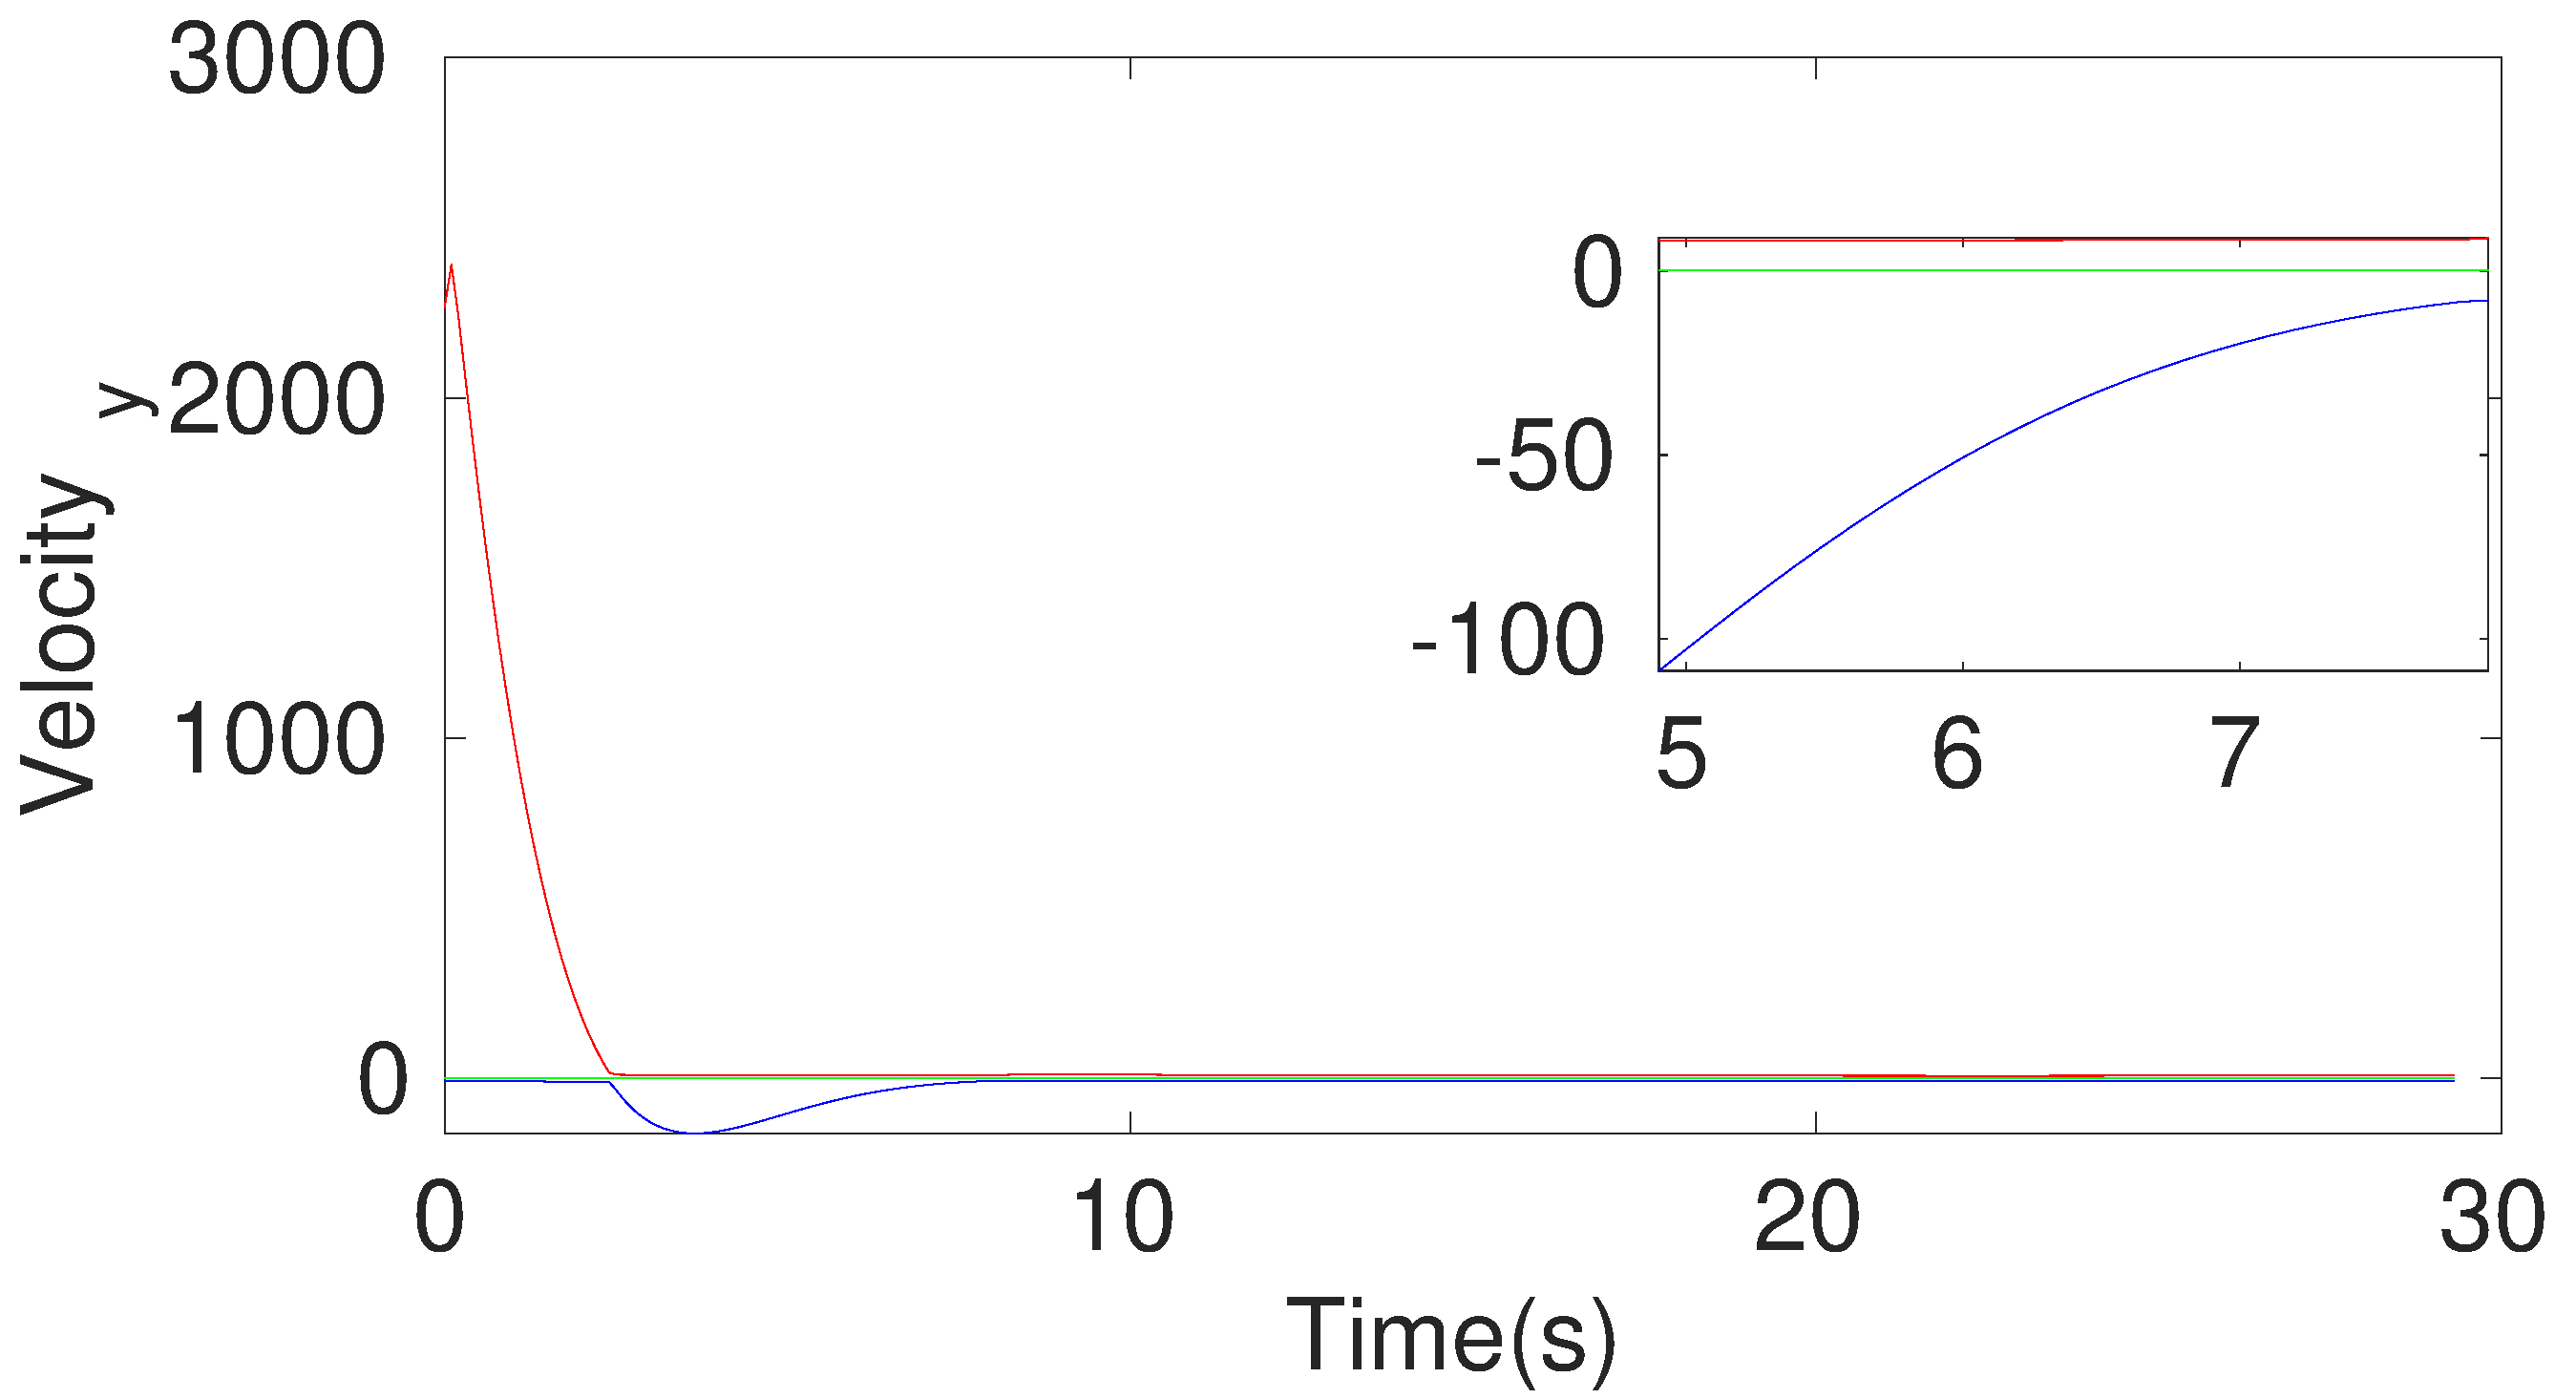
\includegraphics[width=.9\linewidth]{figures/Prad/s3capradVelocity_y}
\end{subfigure}
\begin{subfigure}{.5\linewidth}
\centering
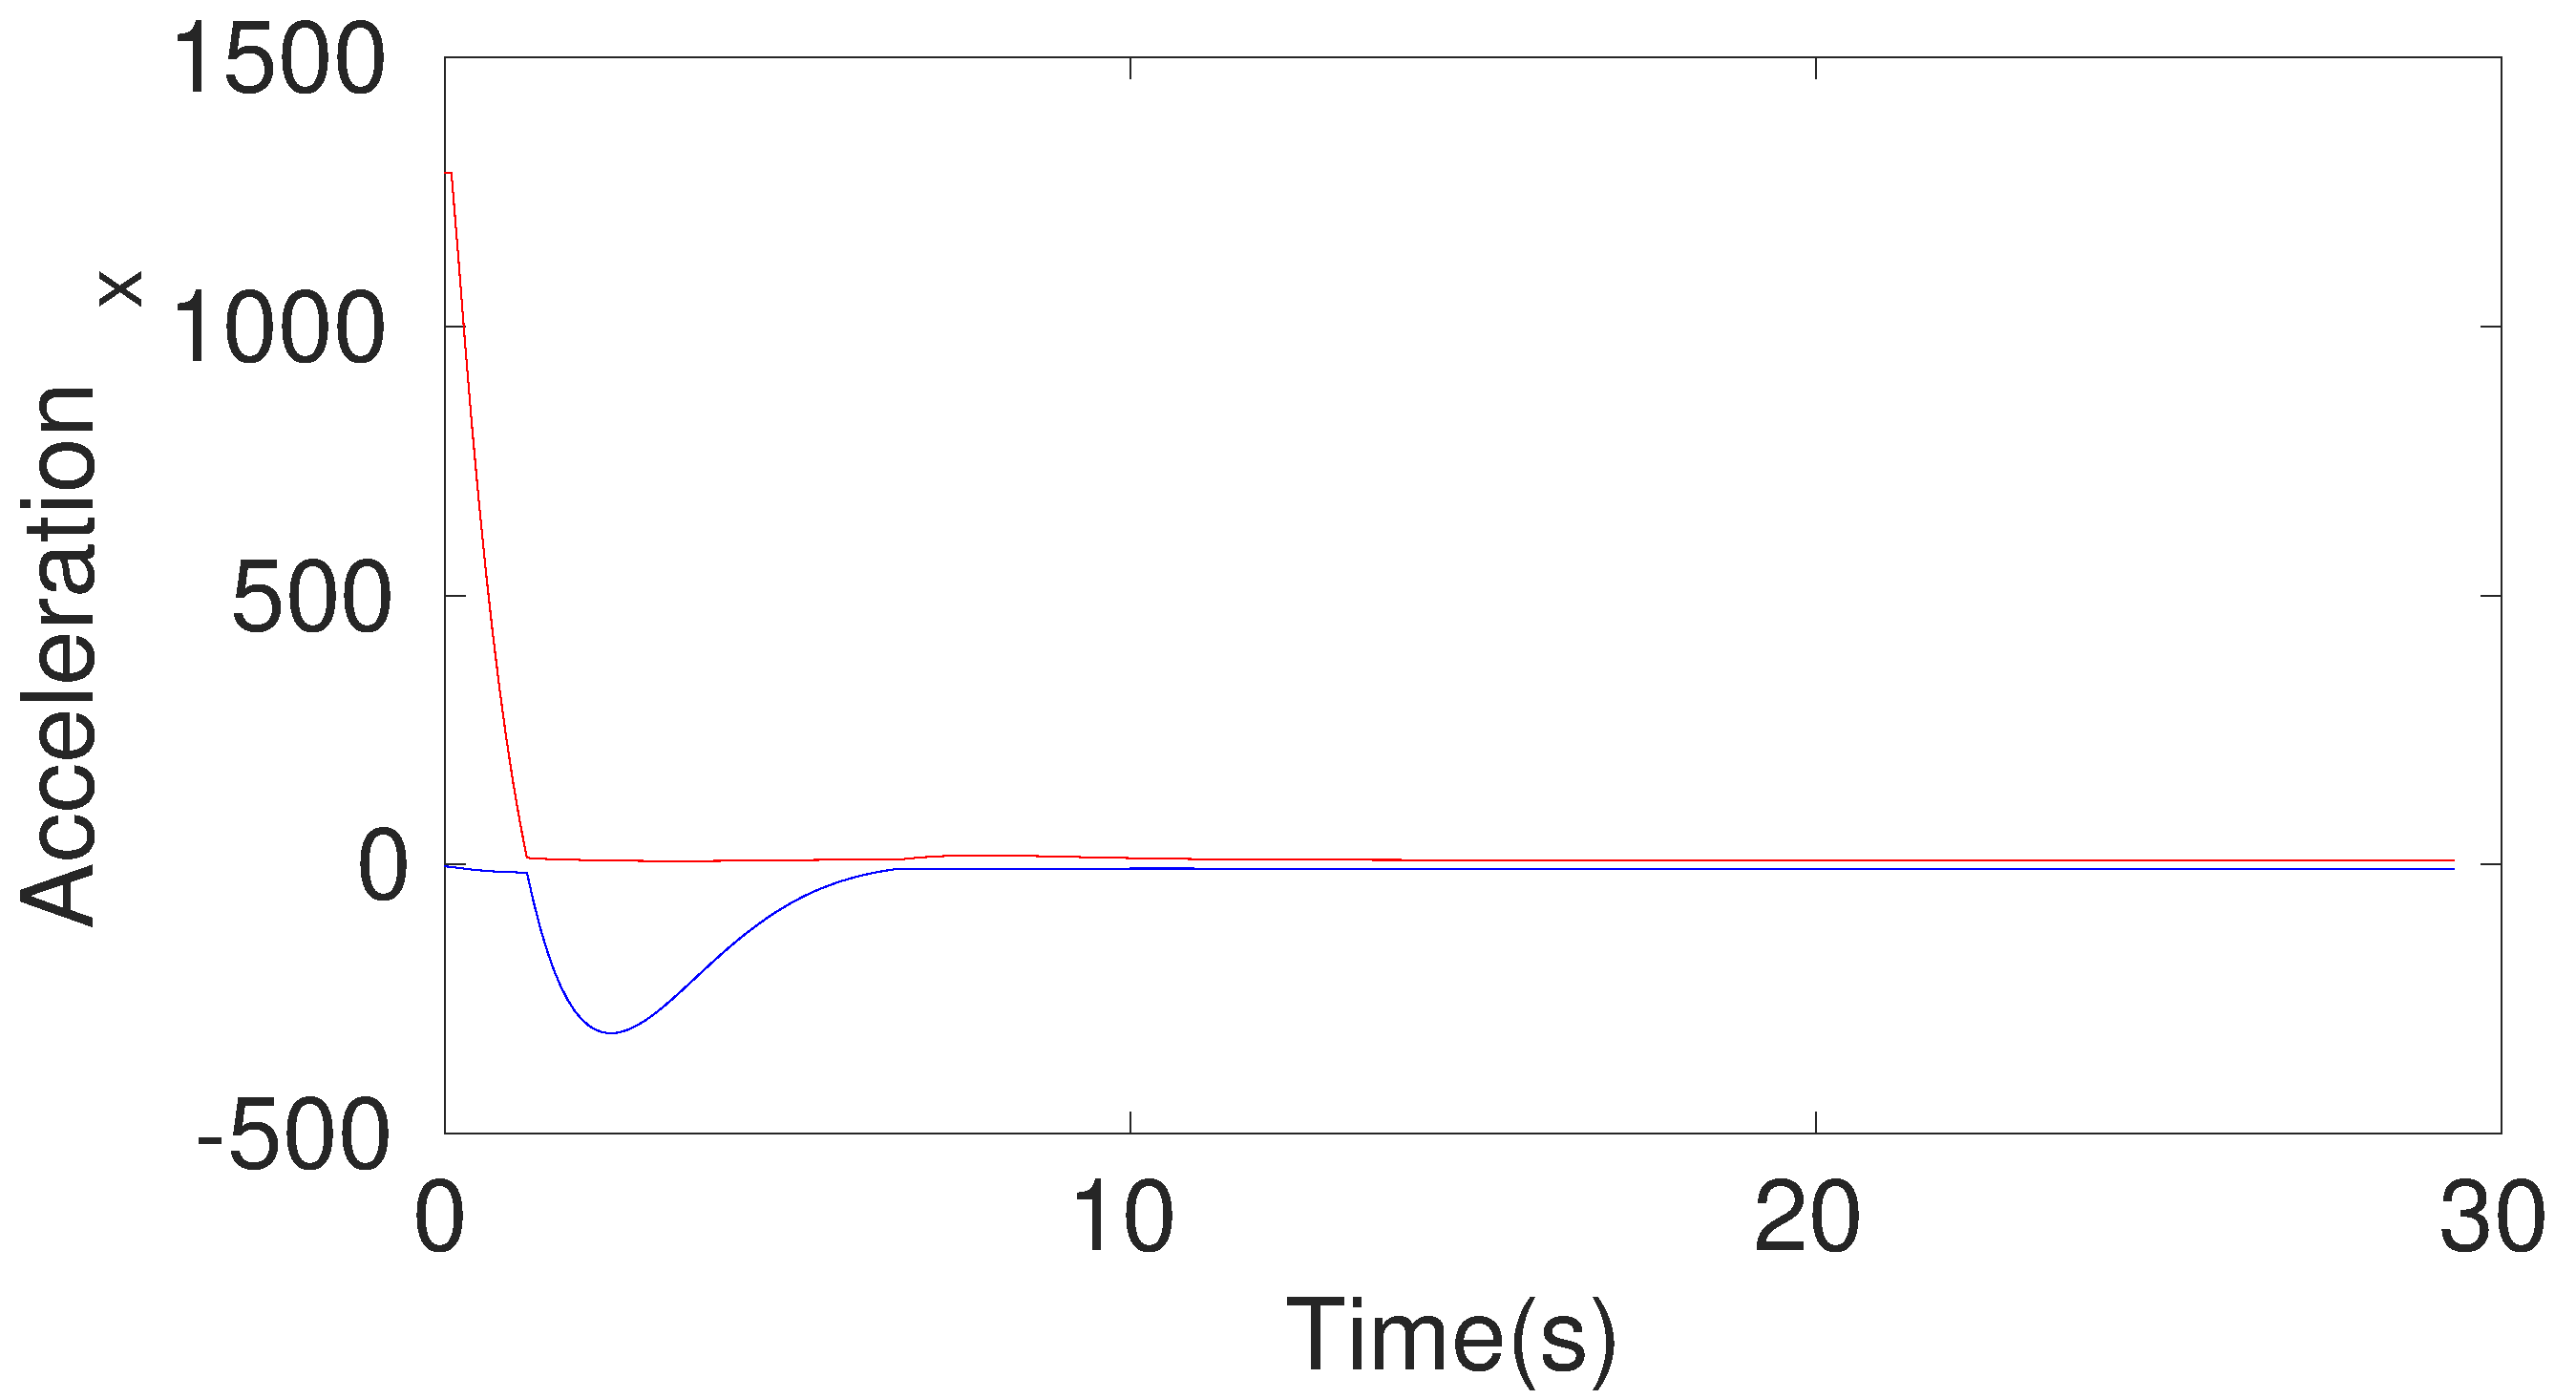
\includegraphics[width=.9\linewidth]{figures/Prad/s3capradAcceleration_x}
\end{subfigure}
\begin{subfigure}{.5\linewidth}
\centering
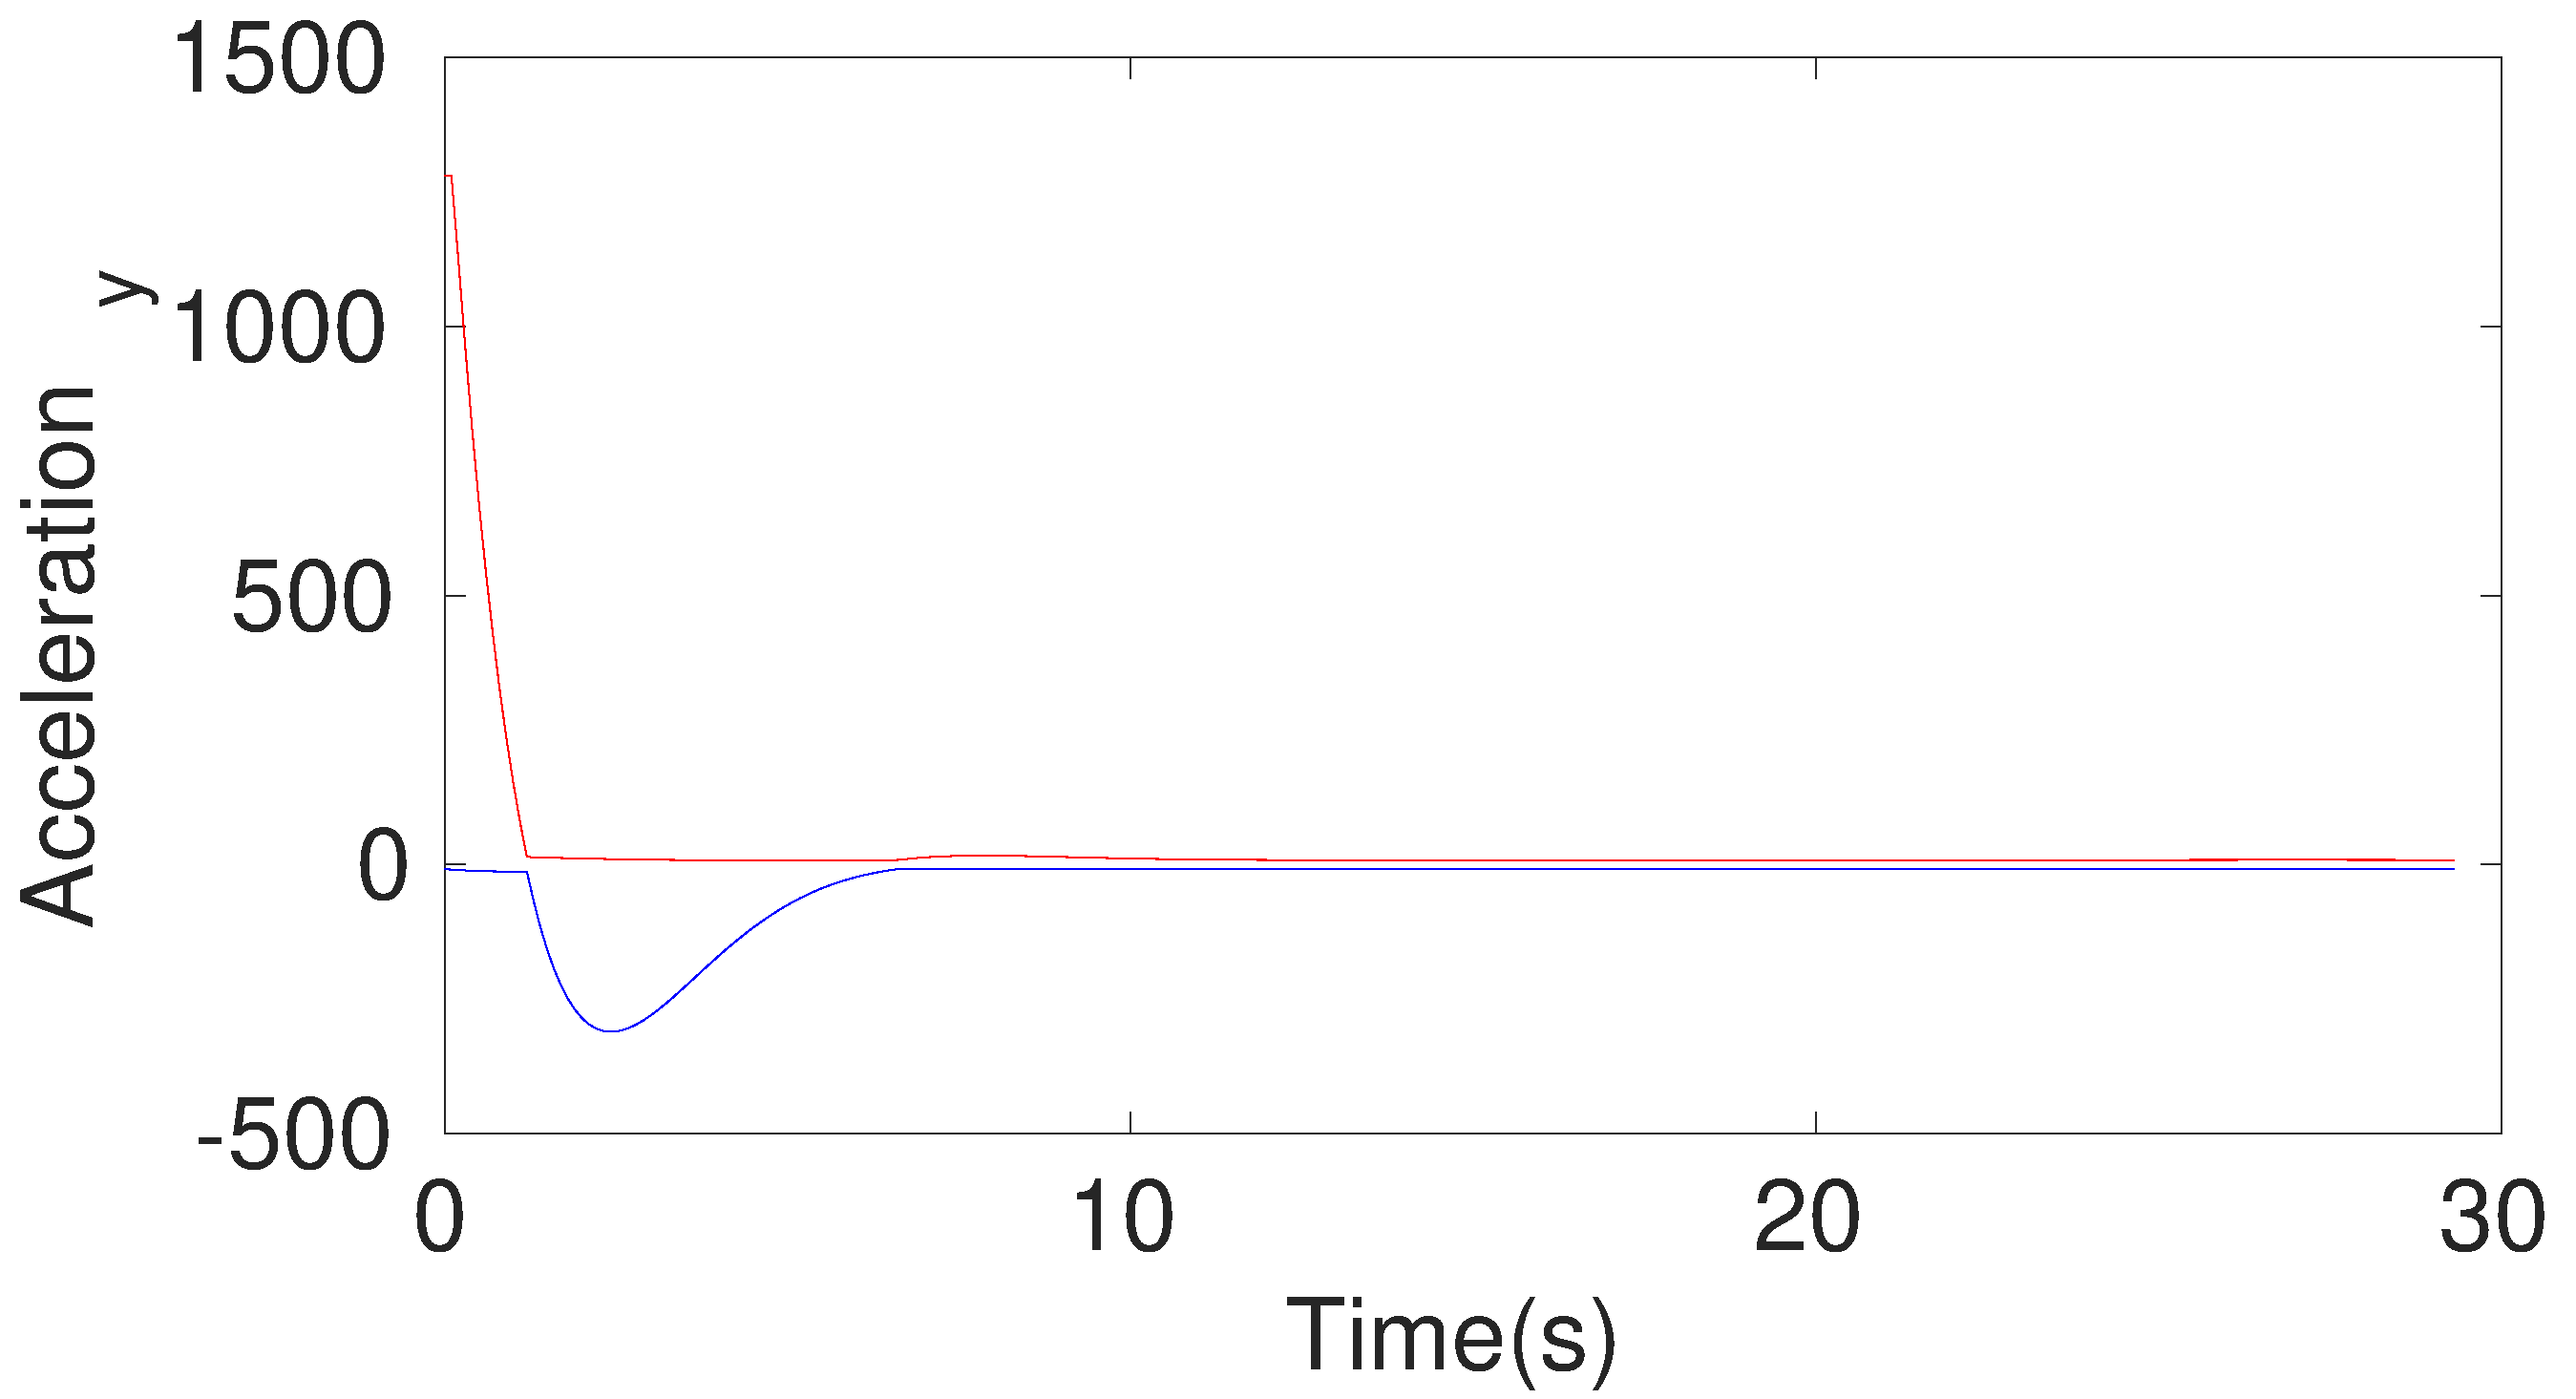
\includegraphics[width=.9\linewidth]{figures/Prad/s3capradAcceleration_y}
\end{subfigure}
\caption{Estimation using Constant Acceleration}
\end{figure}
\begin{figure}[h]
\begin{subfigure}{.5\linewidth}
\centering
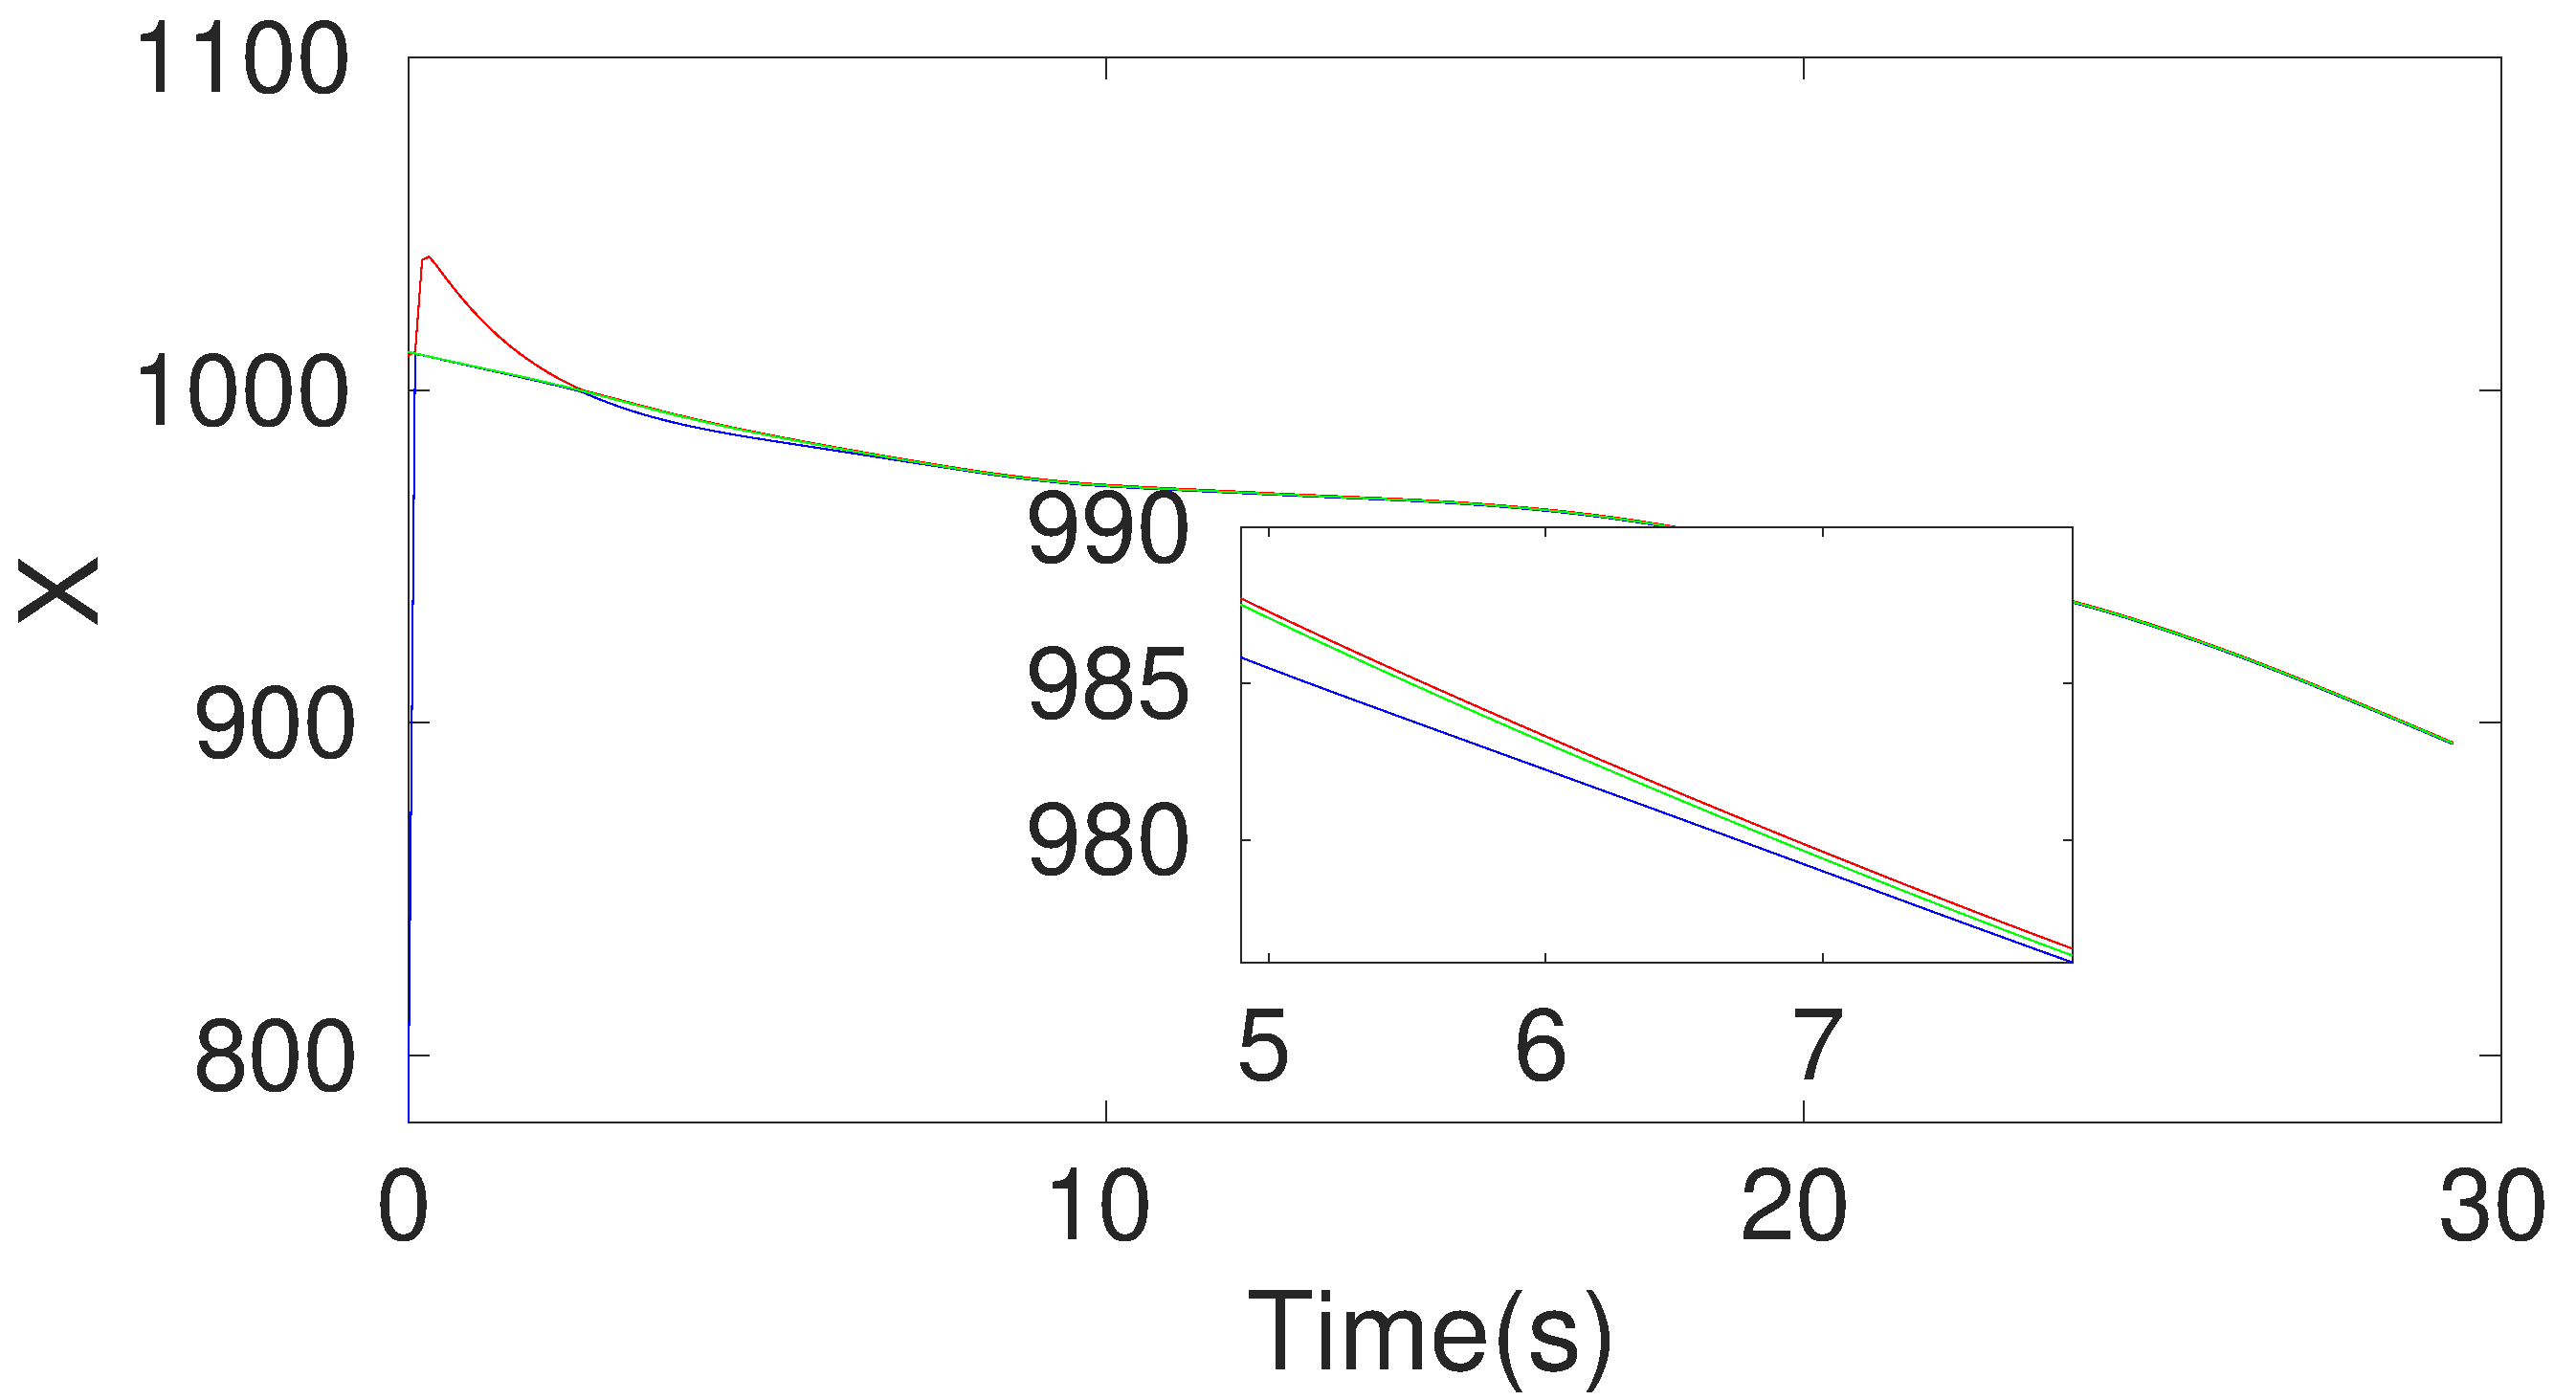
\includegraphics[width=\linewidth]{figures/Prad/s3pmpradX}
\end{subfigure}
\begin{subfigure}{.5\linewidth}
\centering
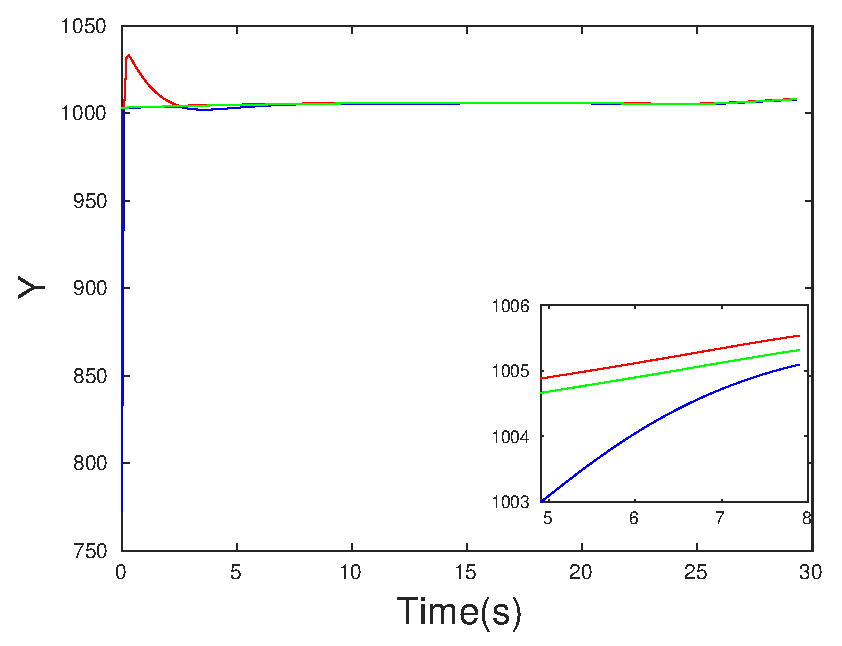
\includegraphics[width=\linewidth]{figures/Prad/s3pmpradY}
\end{subfigure}
\begin{subfigure}{.5\linewidth}
\centering
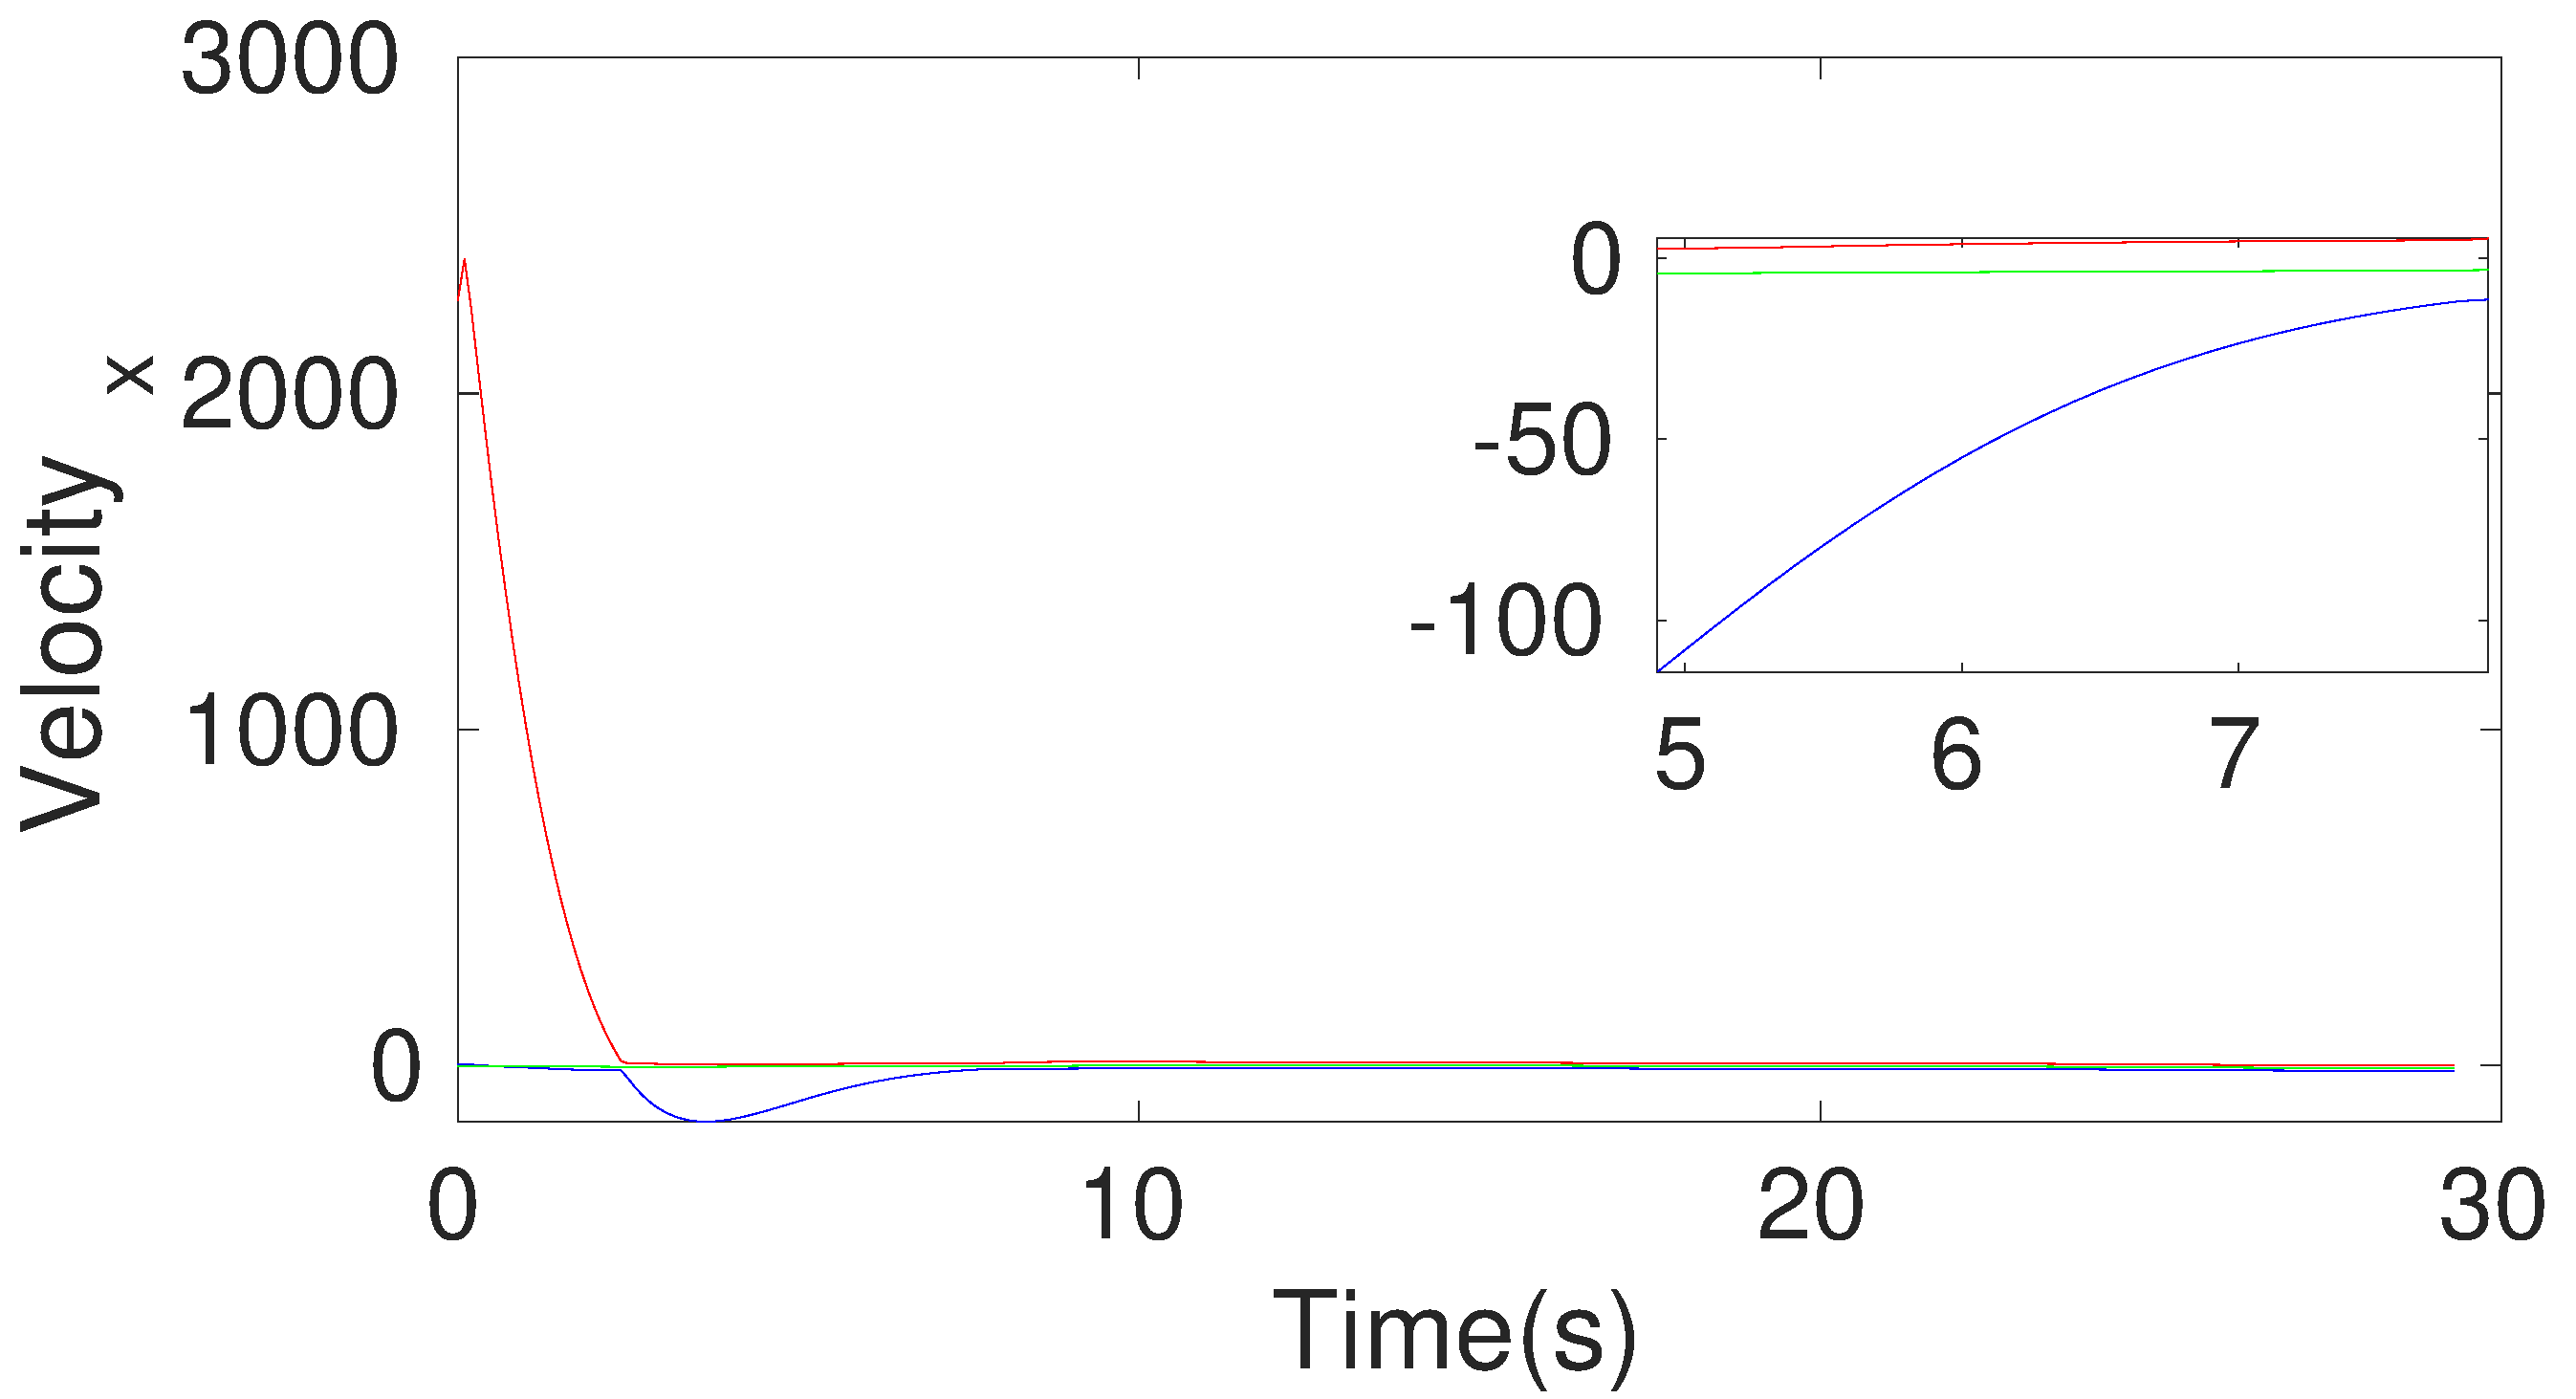
\includegraphics[width=.9\linewidth]{figures/Prad/s3pmpradVelocity_x}
\end{subfigure}
\begin{subfigure}{.5\linewidth}
\centering
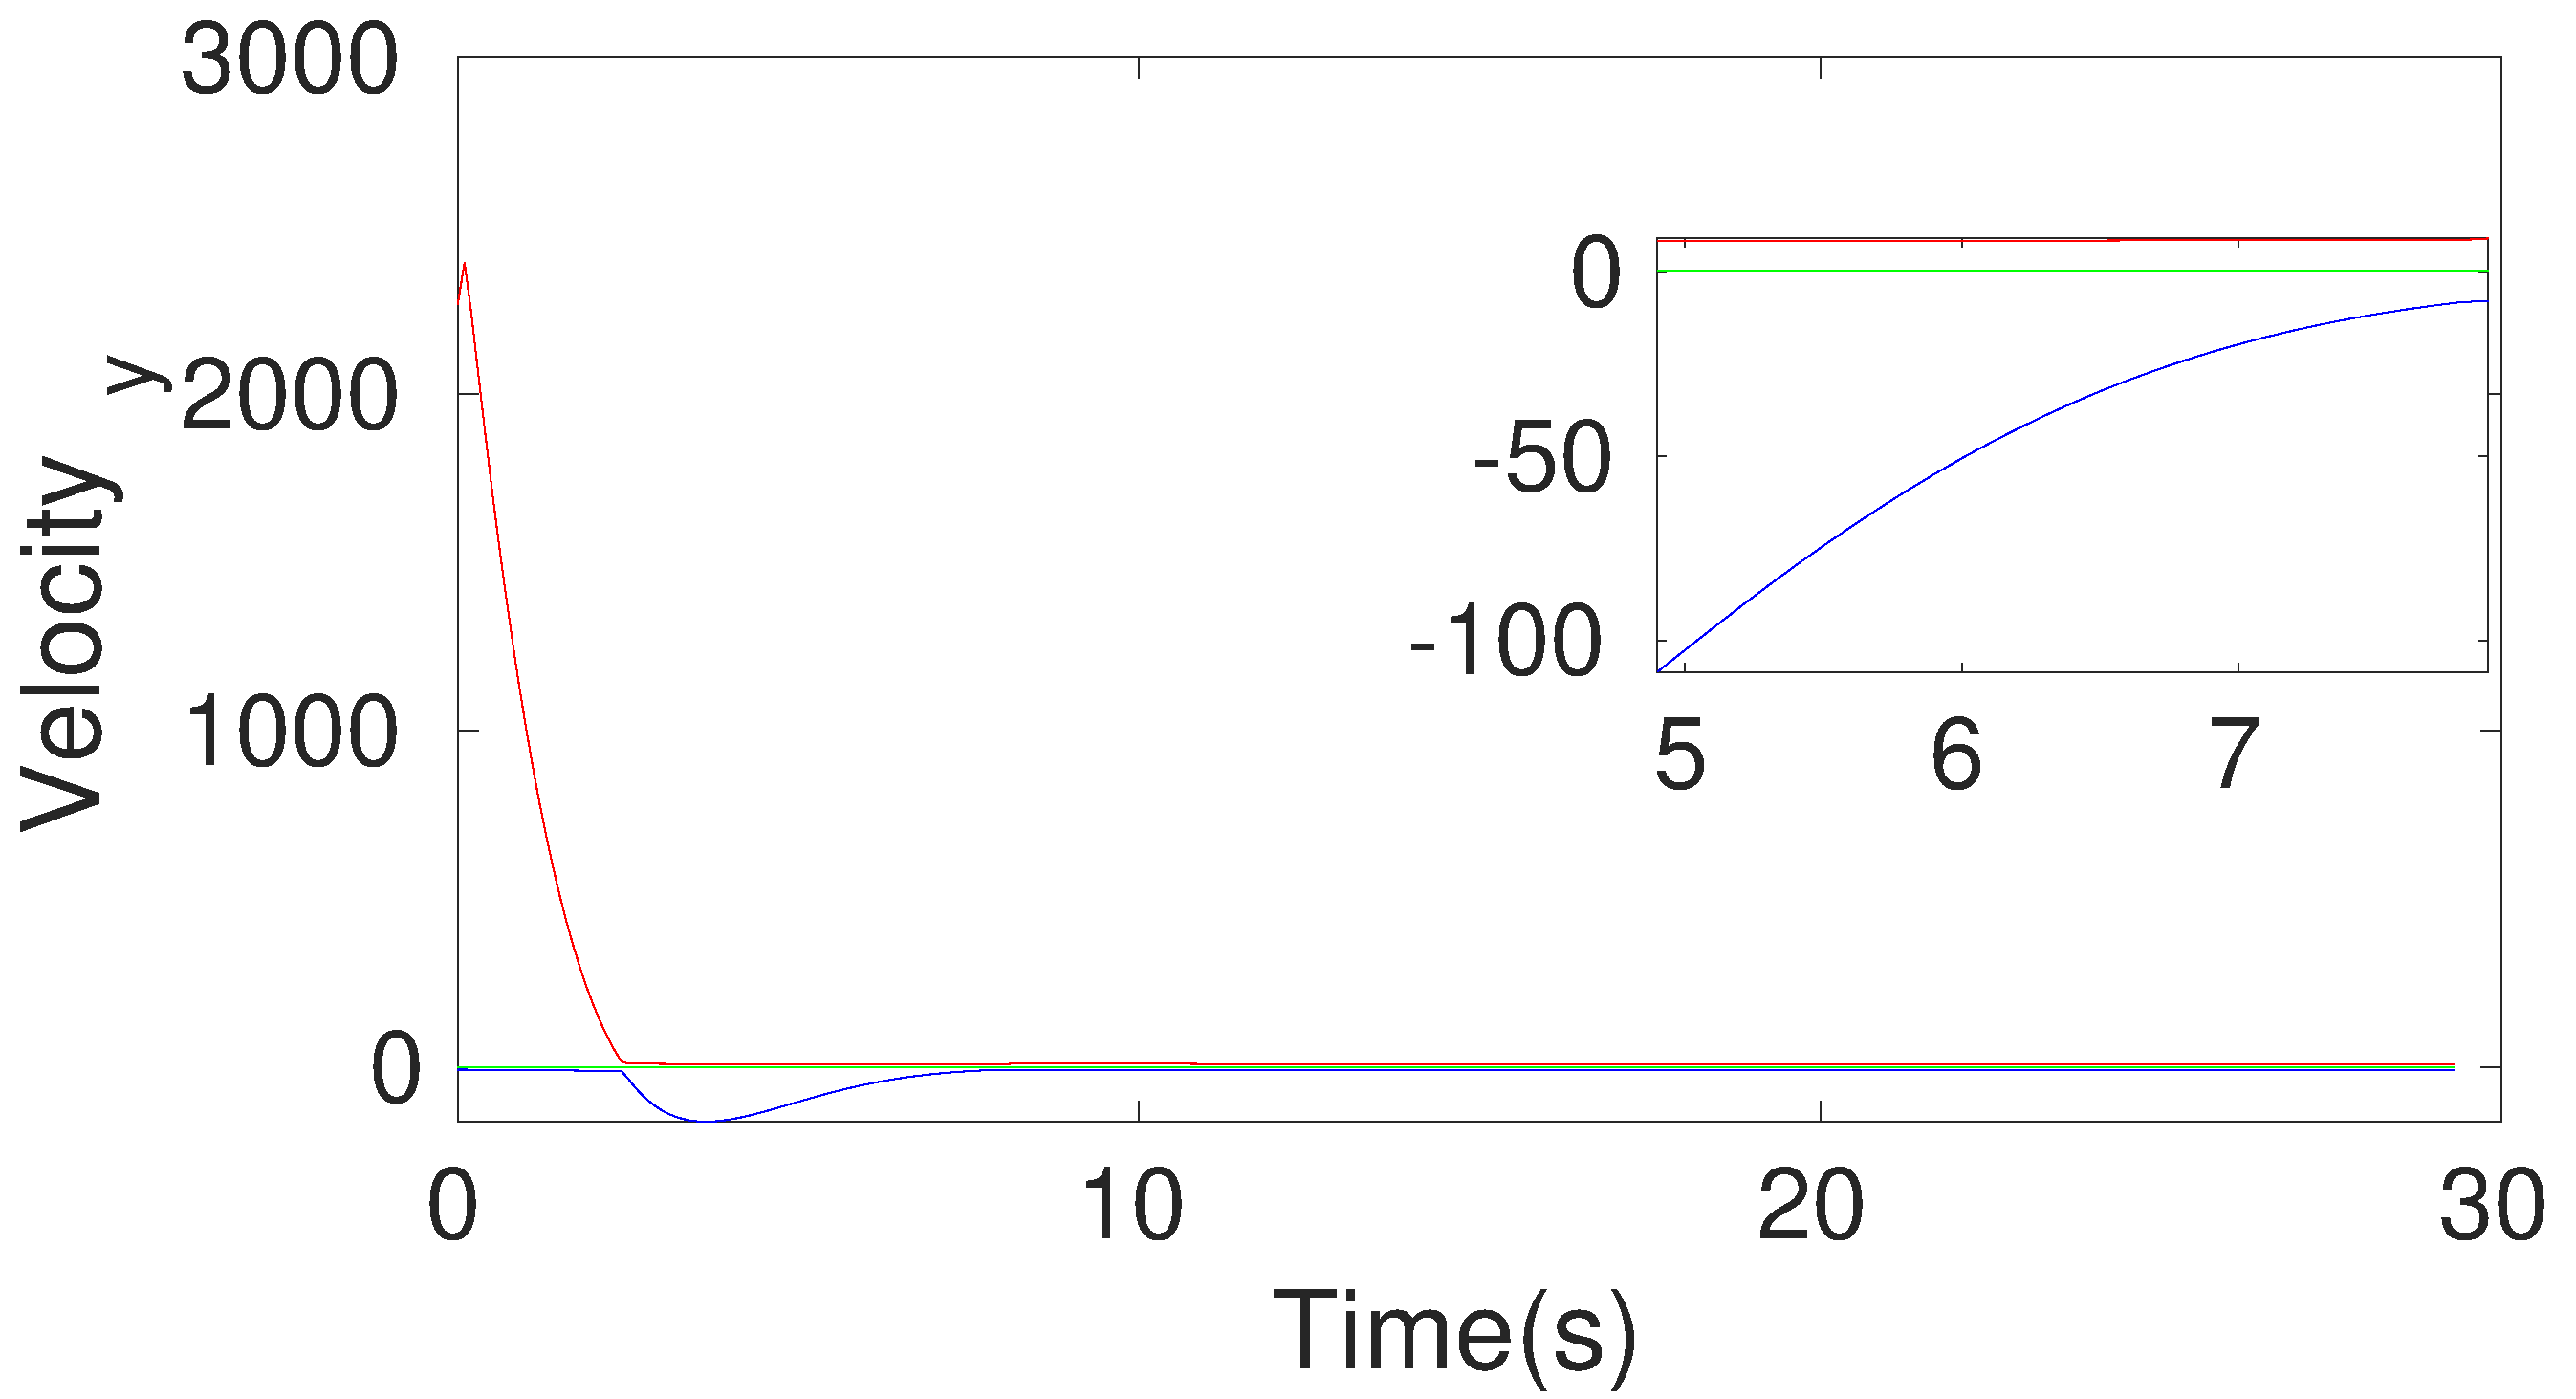
\includegraphics[width=.9\linewidth]{figures/Prad/s3pmpradVelocity_y}
\end{subfigure}
\begin{subfigure}{.5\linewidth}
\centering
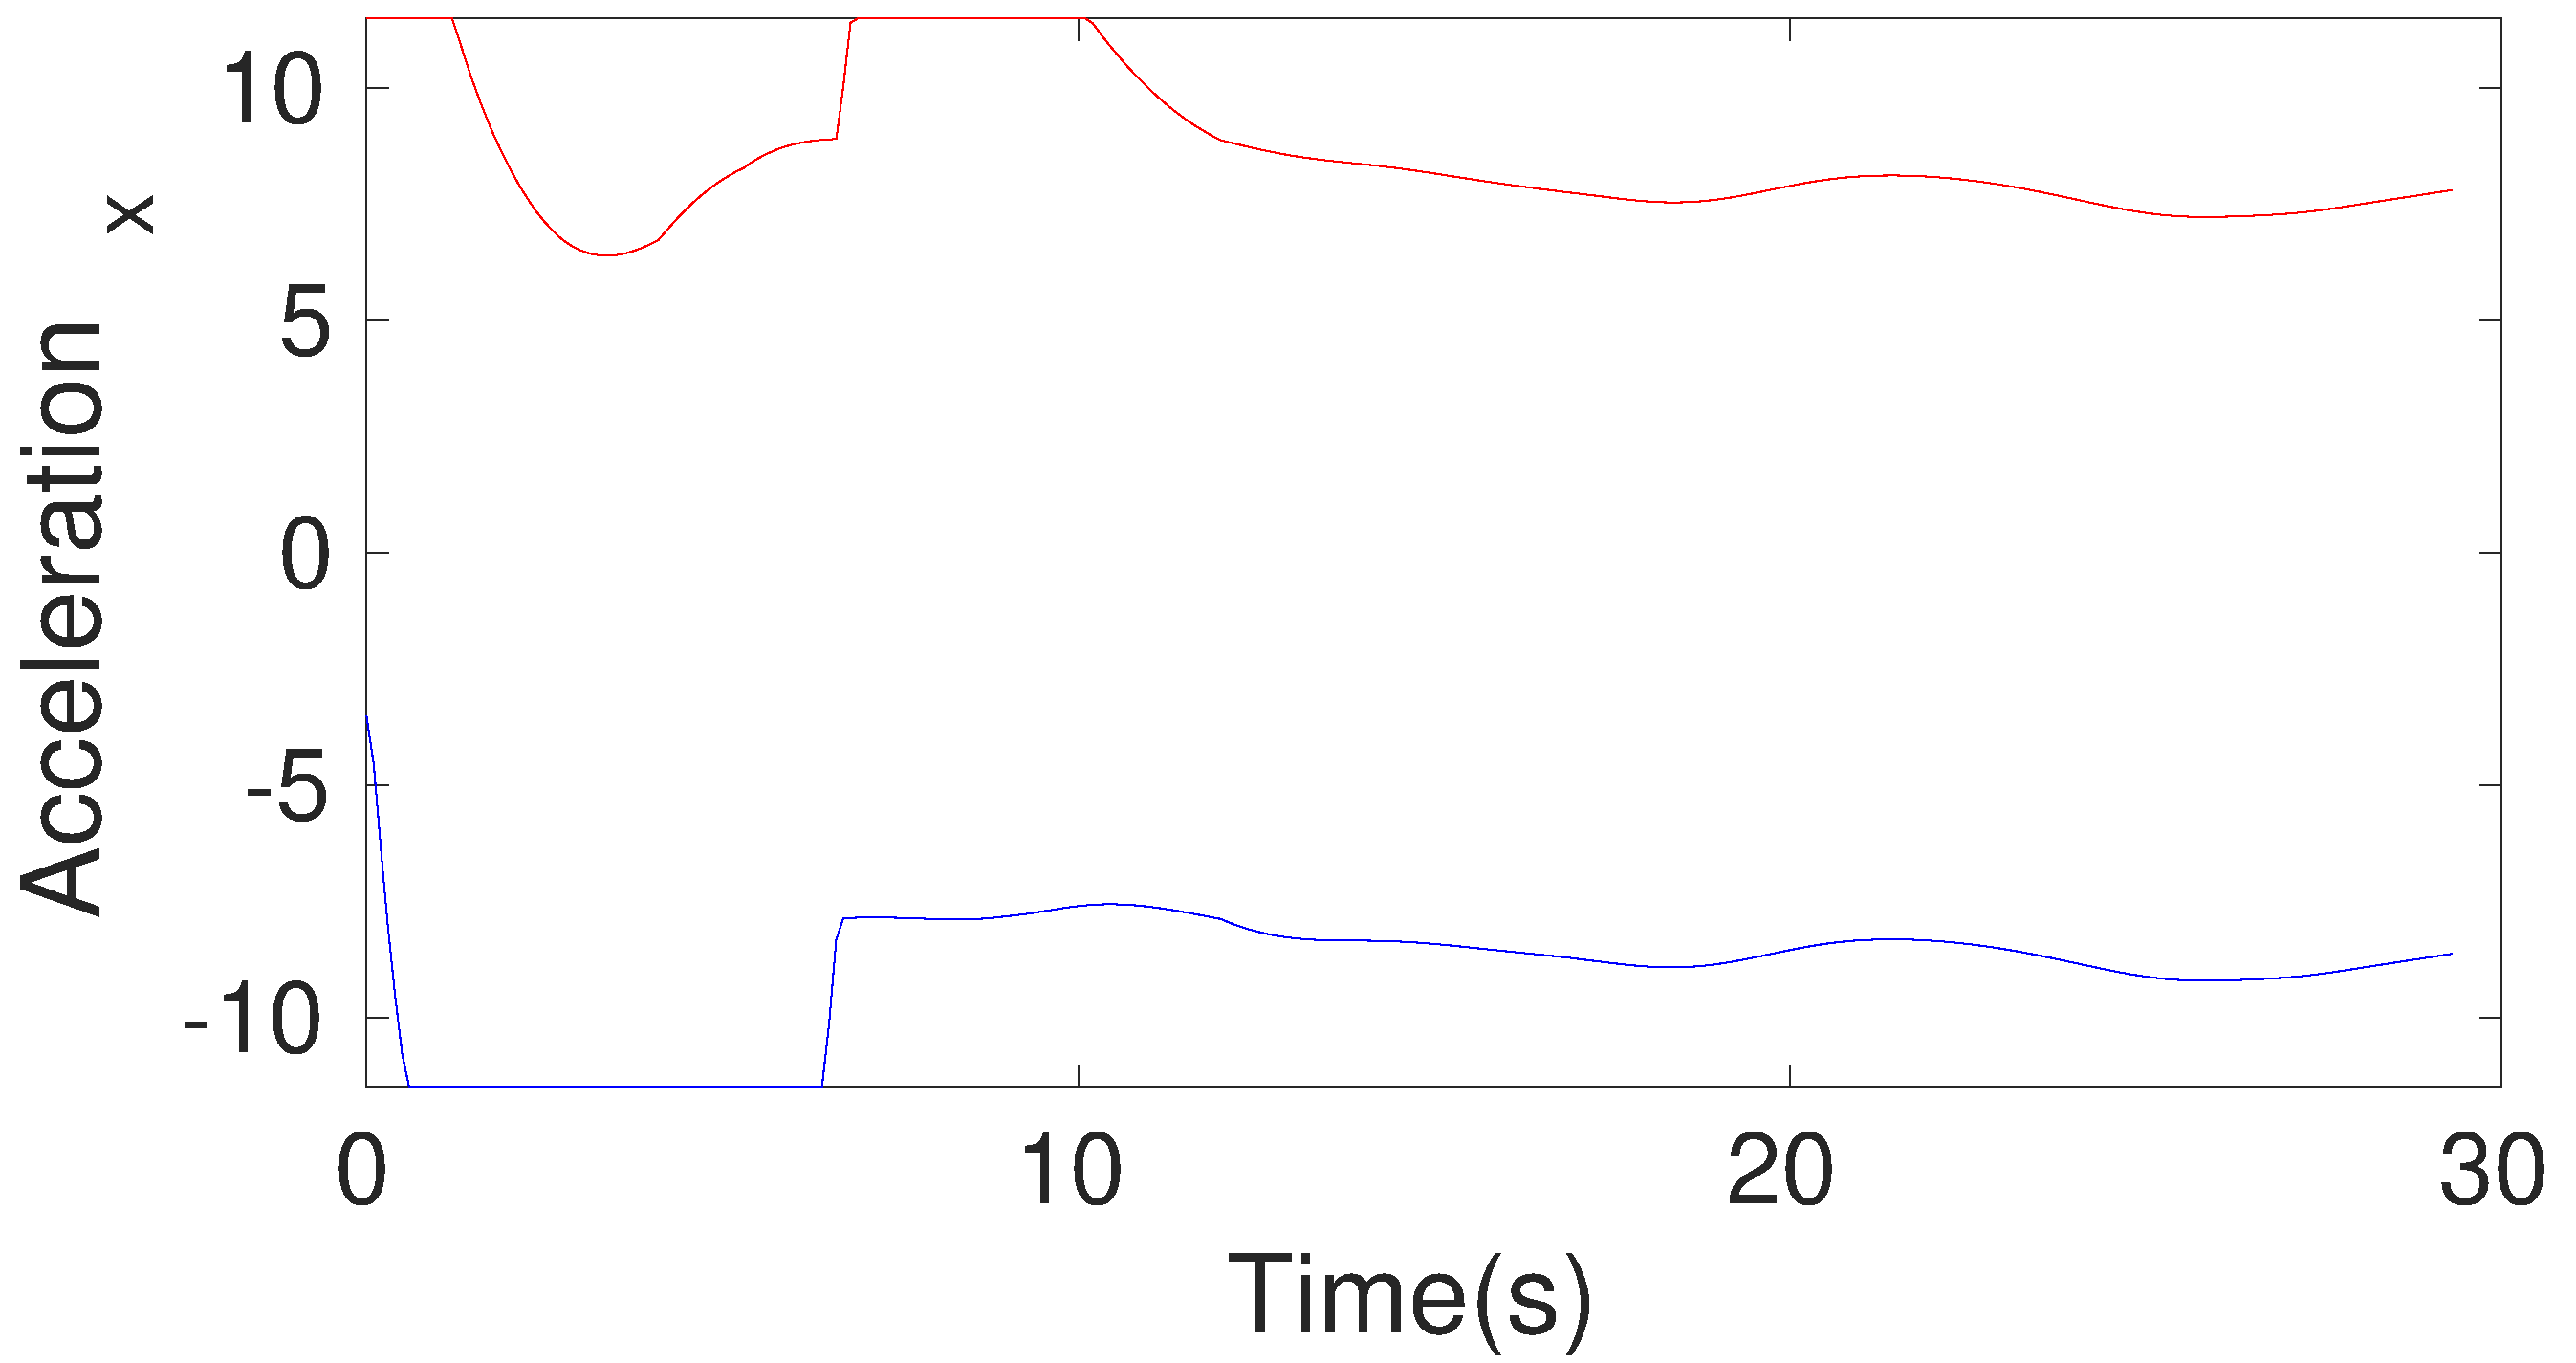
\includegraphics[width=.9\linewidth]{figures/Prad/s3pmpradAcceleration_x}
\end{subfigure}
\begin{subfigure}{.5\linewidth}
\centering
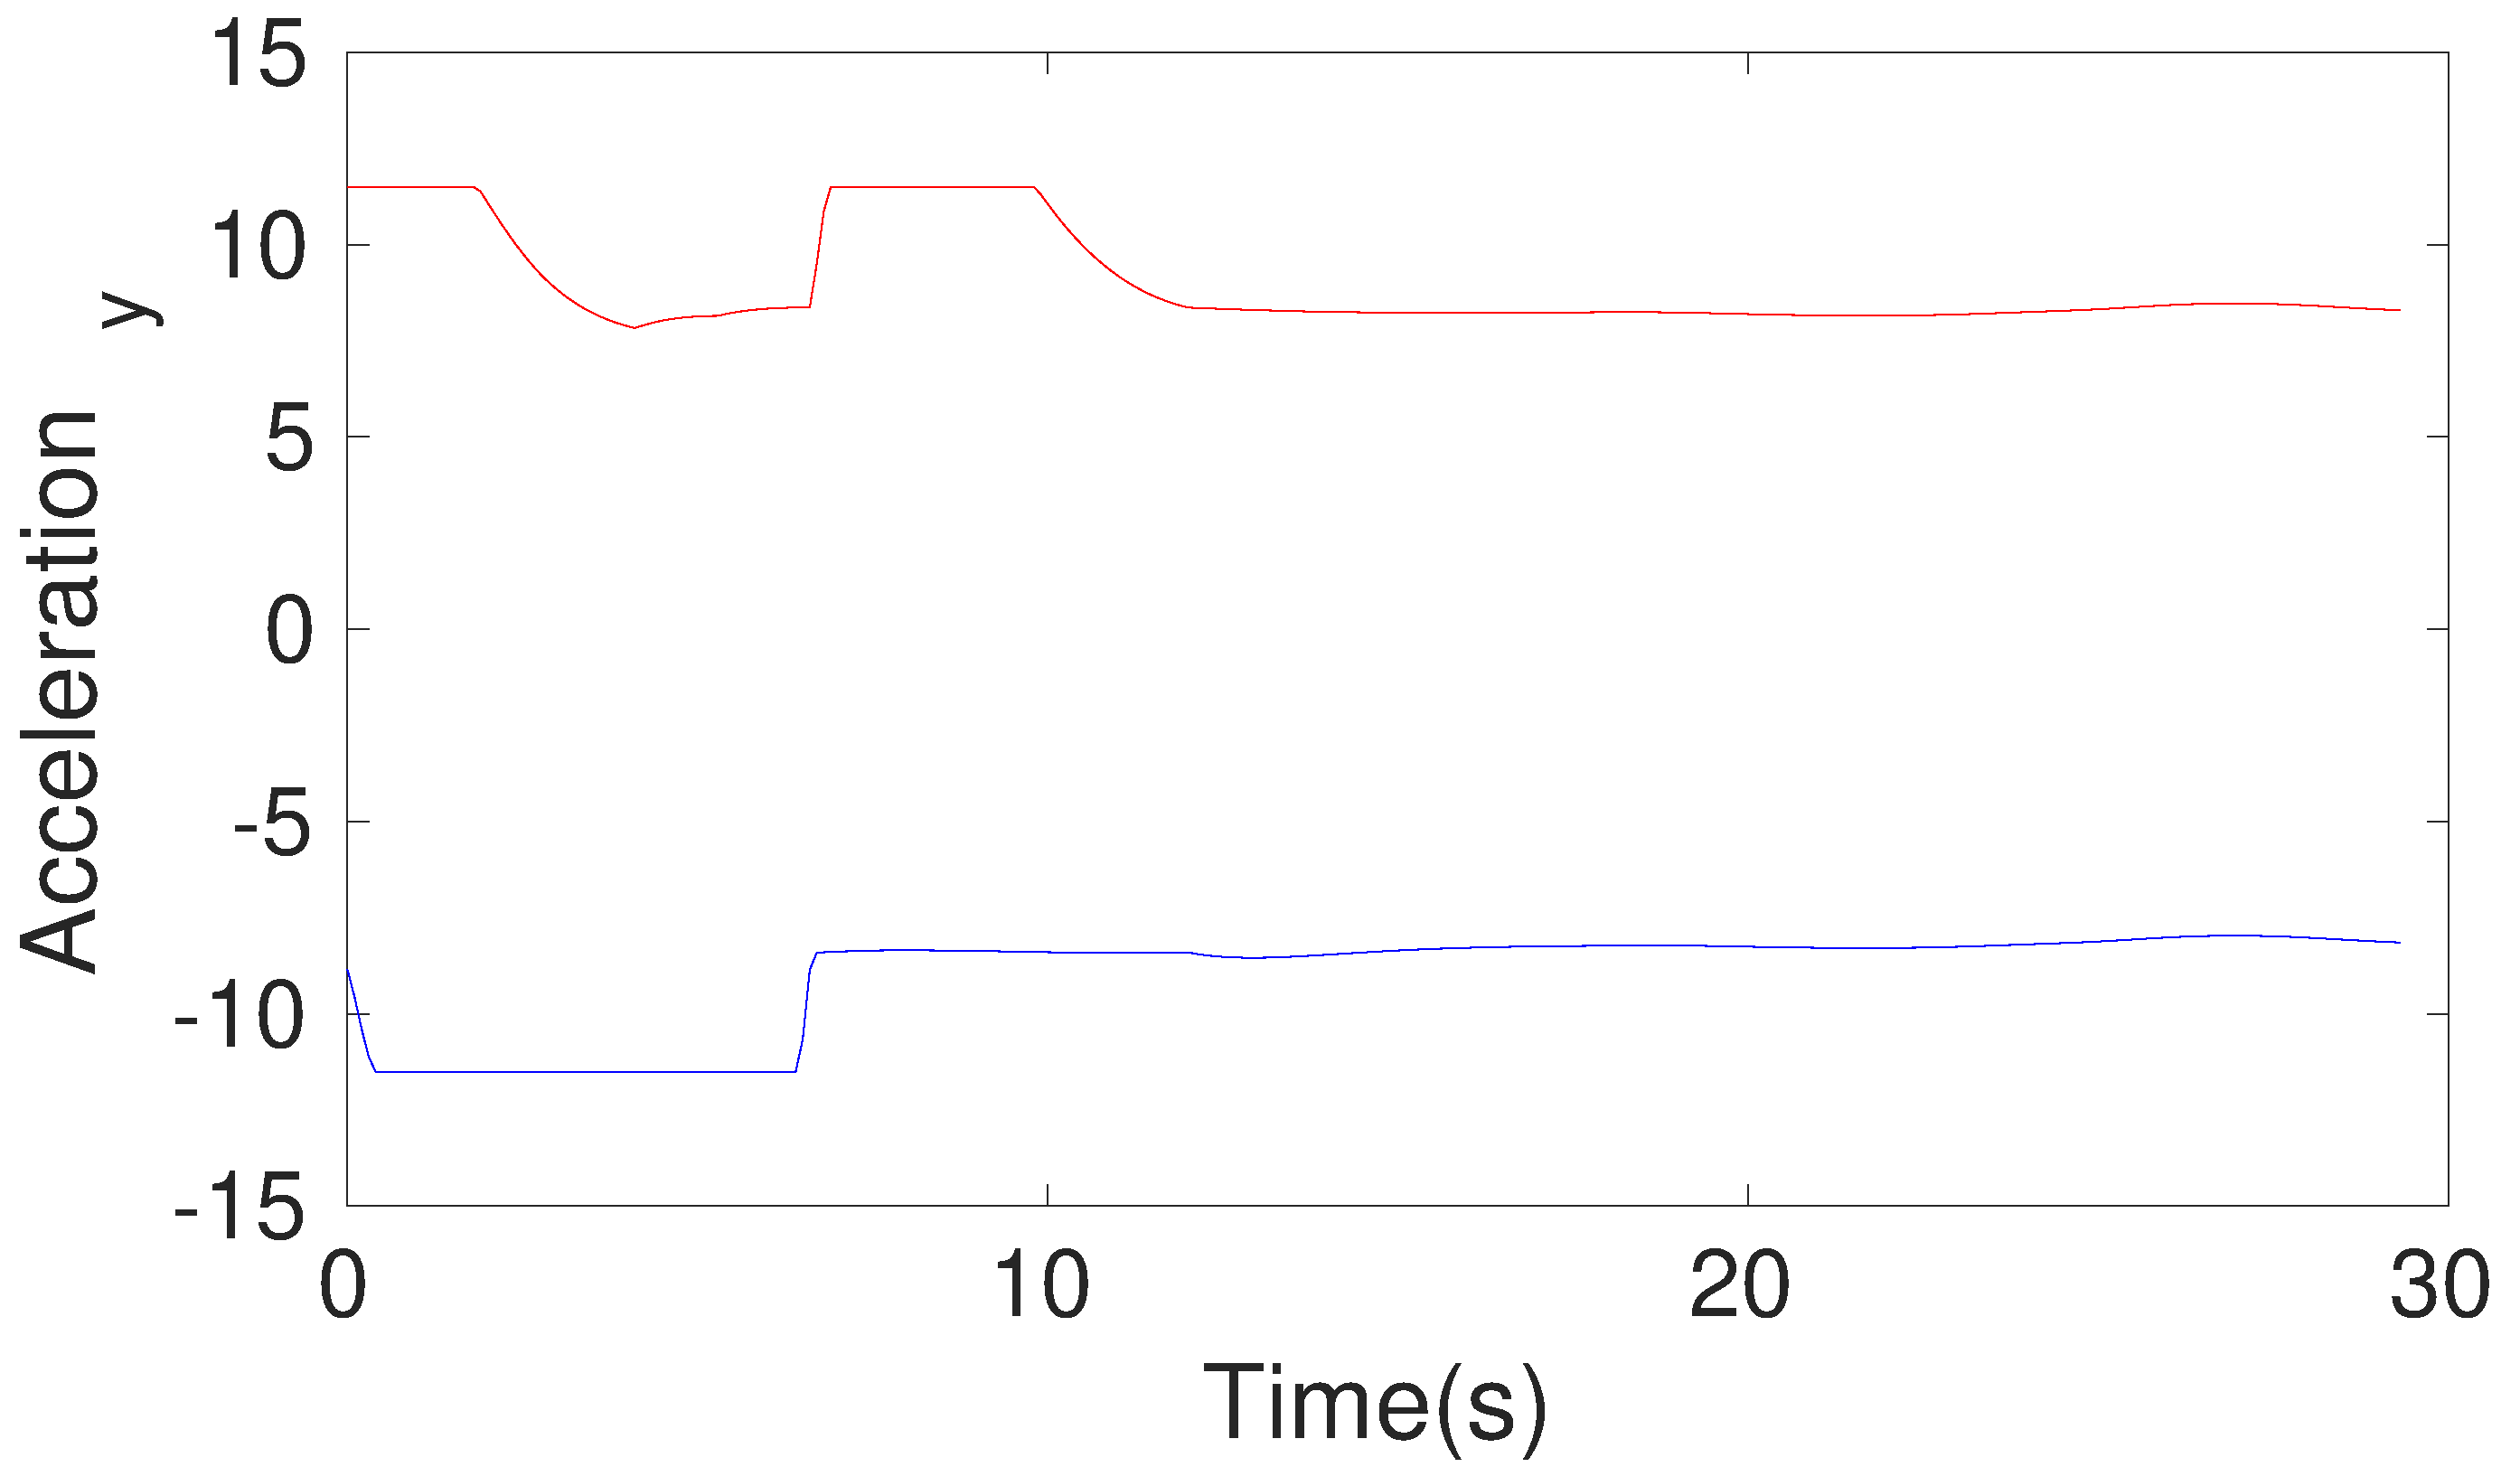
\includegraphics[width=.9\linewidth]{figures/Prad/s3pmpradAcceleration_y}
\end{subfigure}
\caption{Estimation using Point Mass Model}
\end{figure}


\clearpage
\subsection{Interval Observer using H-$\infty$}
\FloatBarrier
\begin{figure}[h]
\begin{subfigure}{.5\linewidth}
\centering
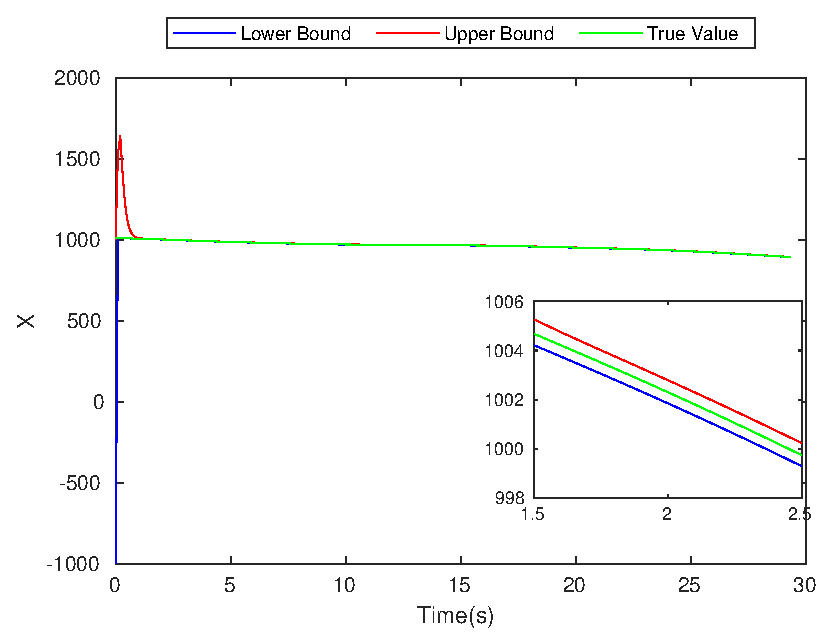
\includegraphics[width=.9\linewidth]{figures/HInf/s3cvHInfX}
\end{subfigure}
\begin{subfigure}{.5\linewidth}
\centering
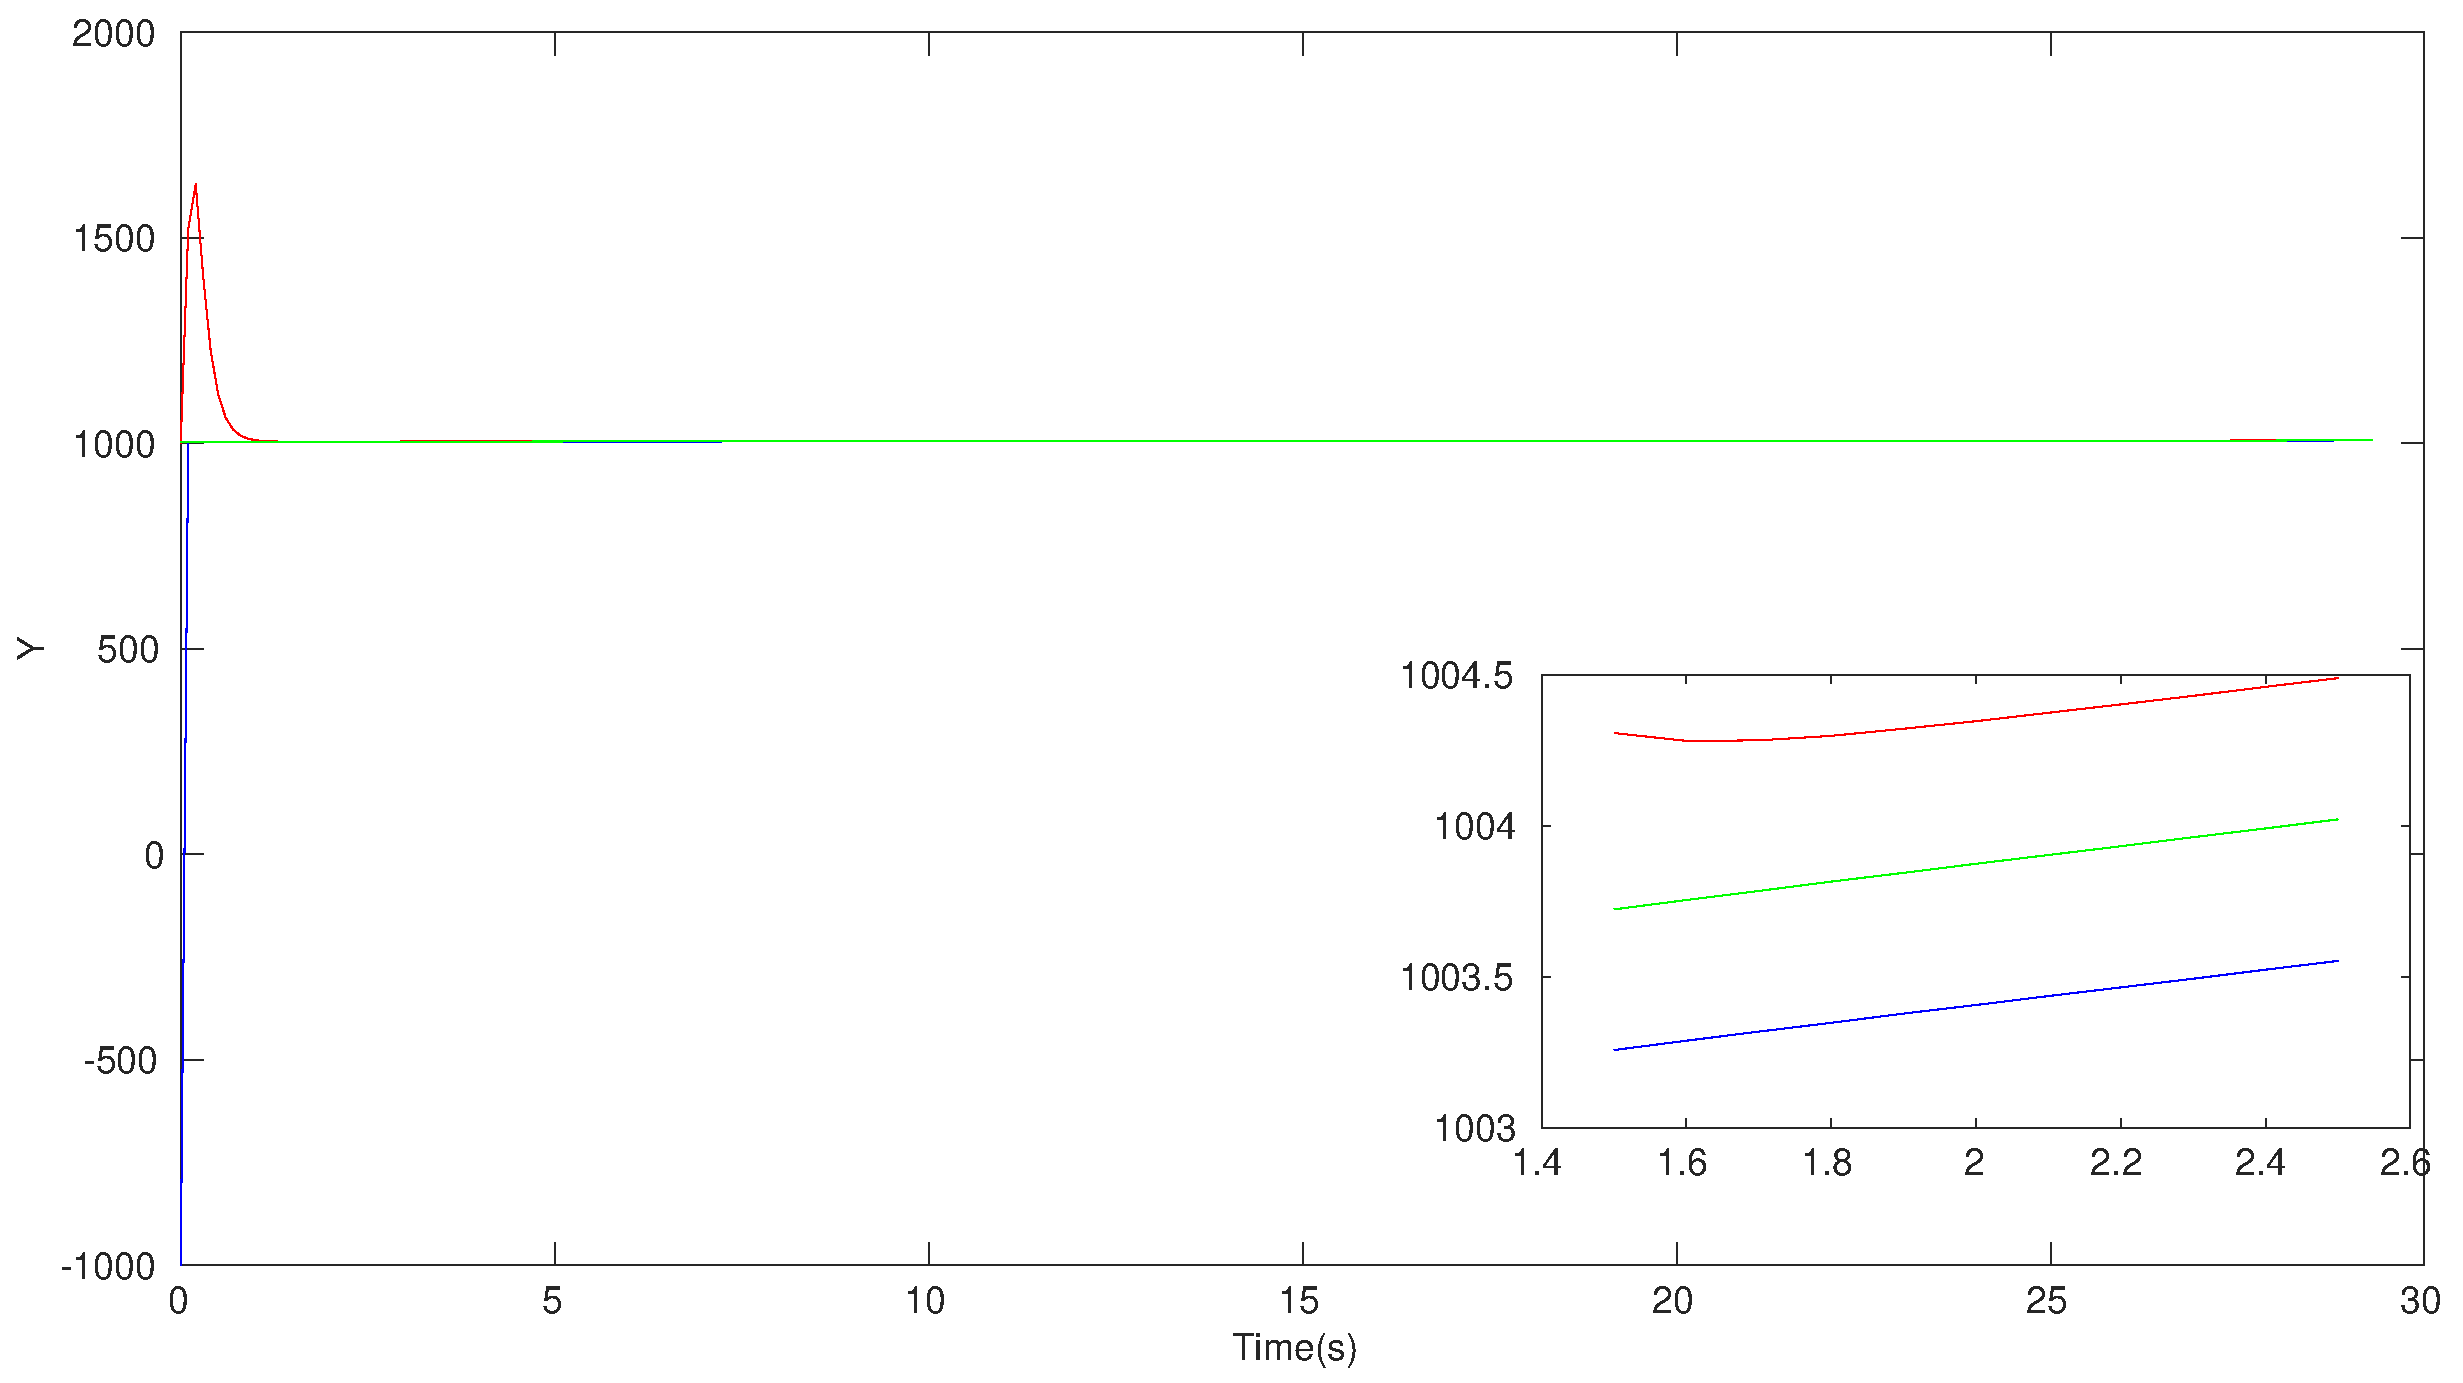
\includegraphics[width=.9\linewidth]{figures/HInf/s3cvHInfY}
\end{subfigure}
\begin{subfigure}{.5\linewidth}
\centering
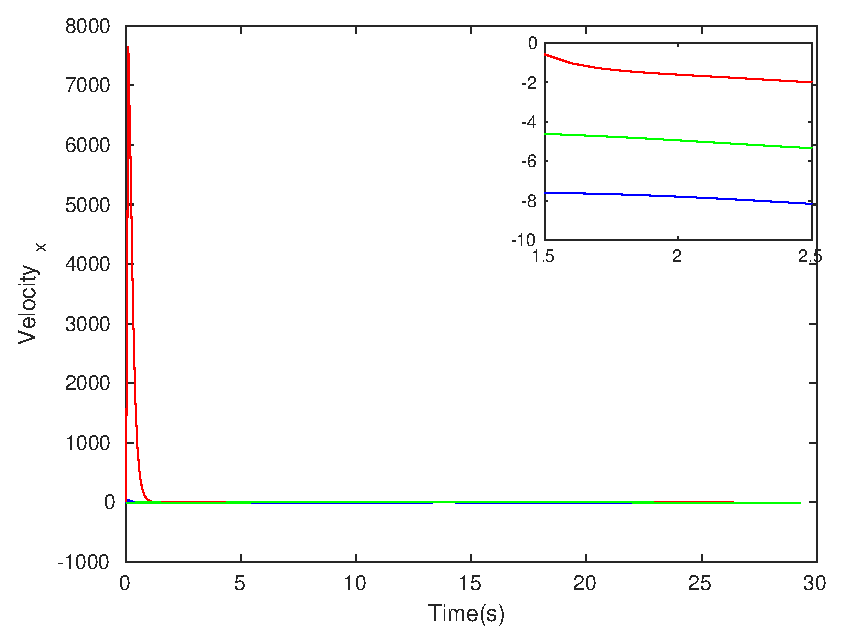
\includegraphics[width=.9\linewidth]{figures/HInf/s3cvHInfVelocity_x}
\end{subfigure}
\begin{subfigure}{.5\linewidth}
\centering
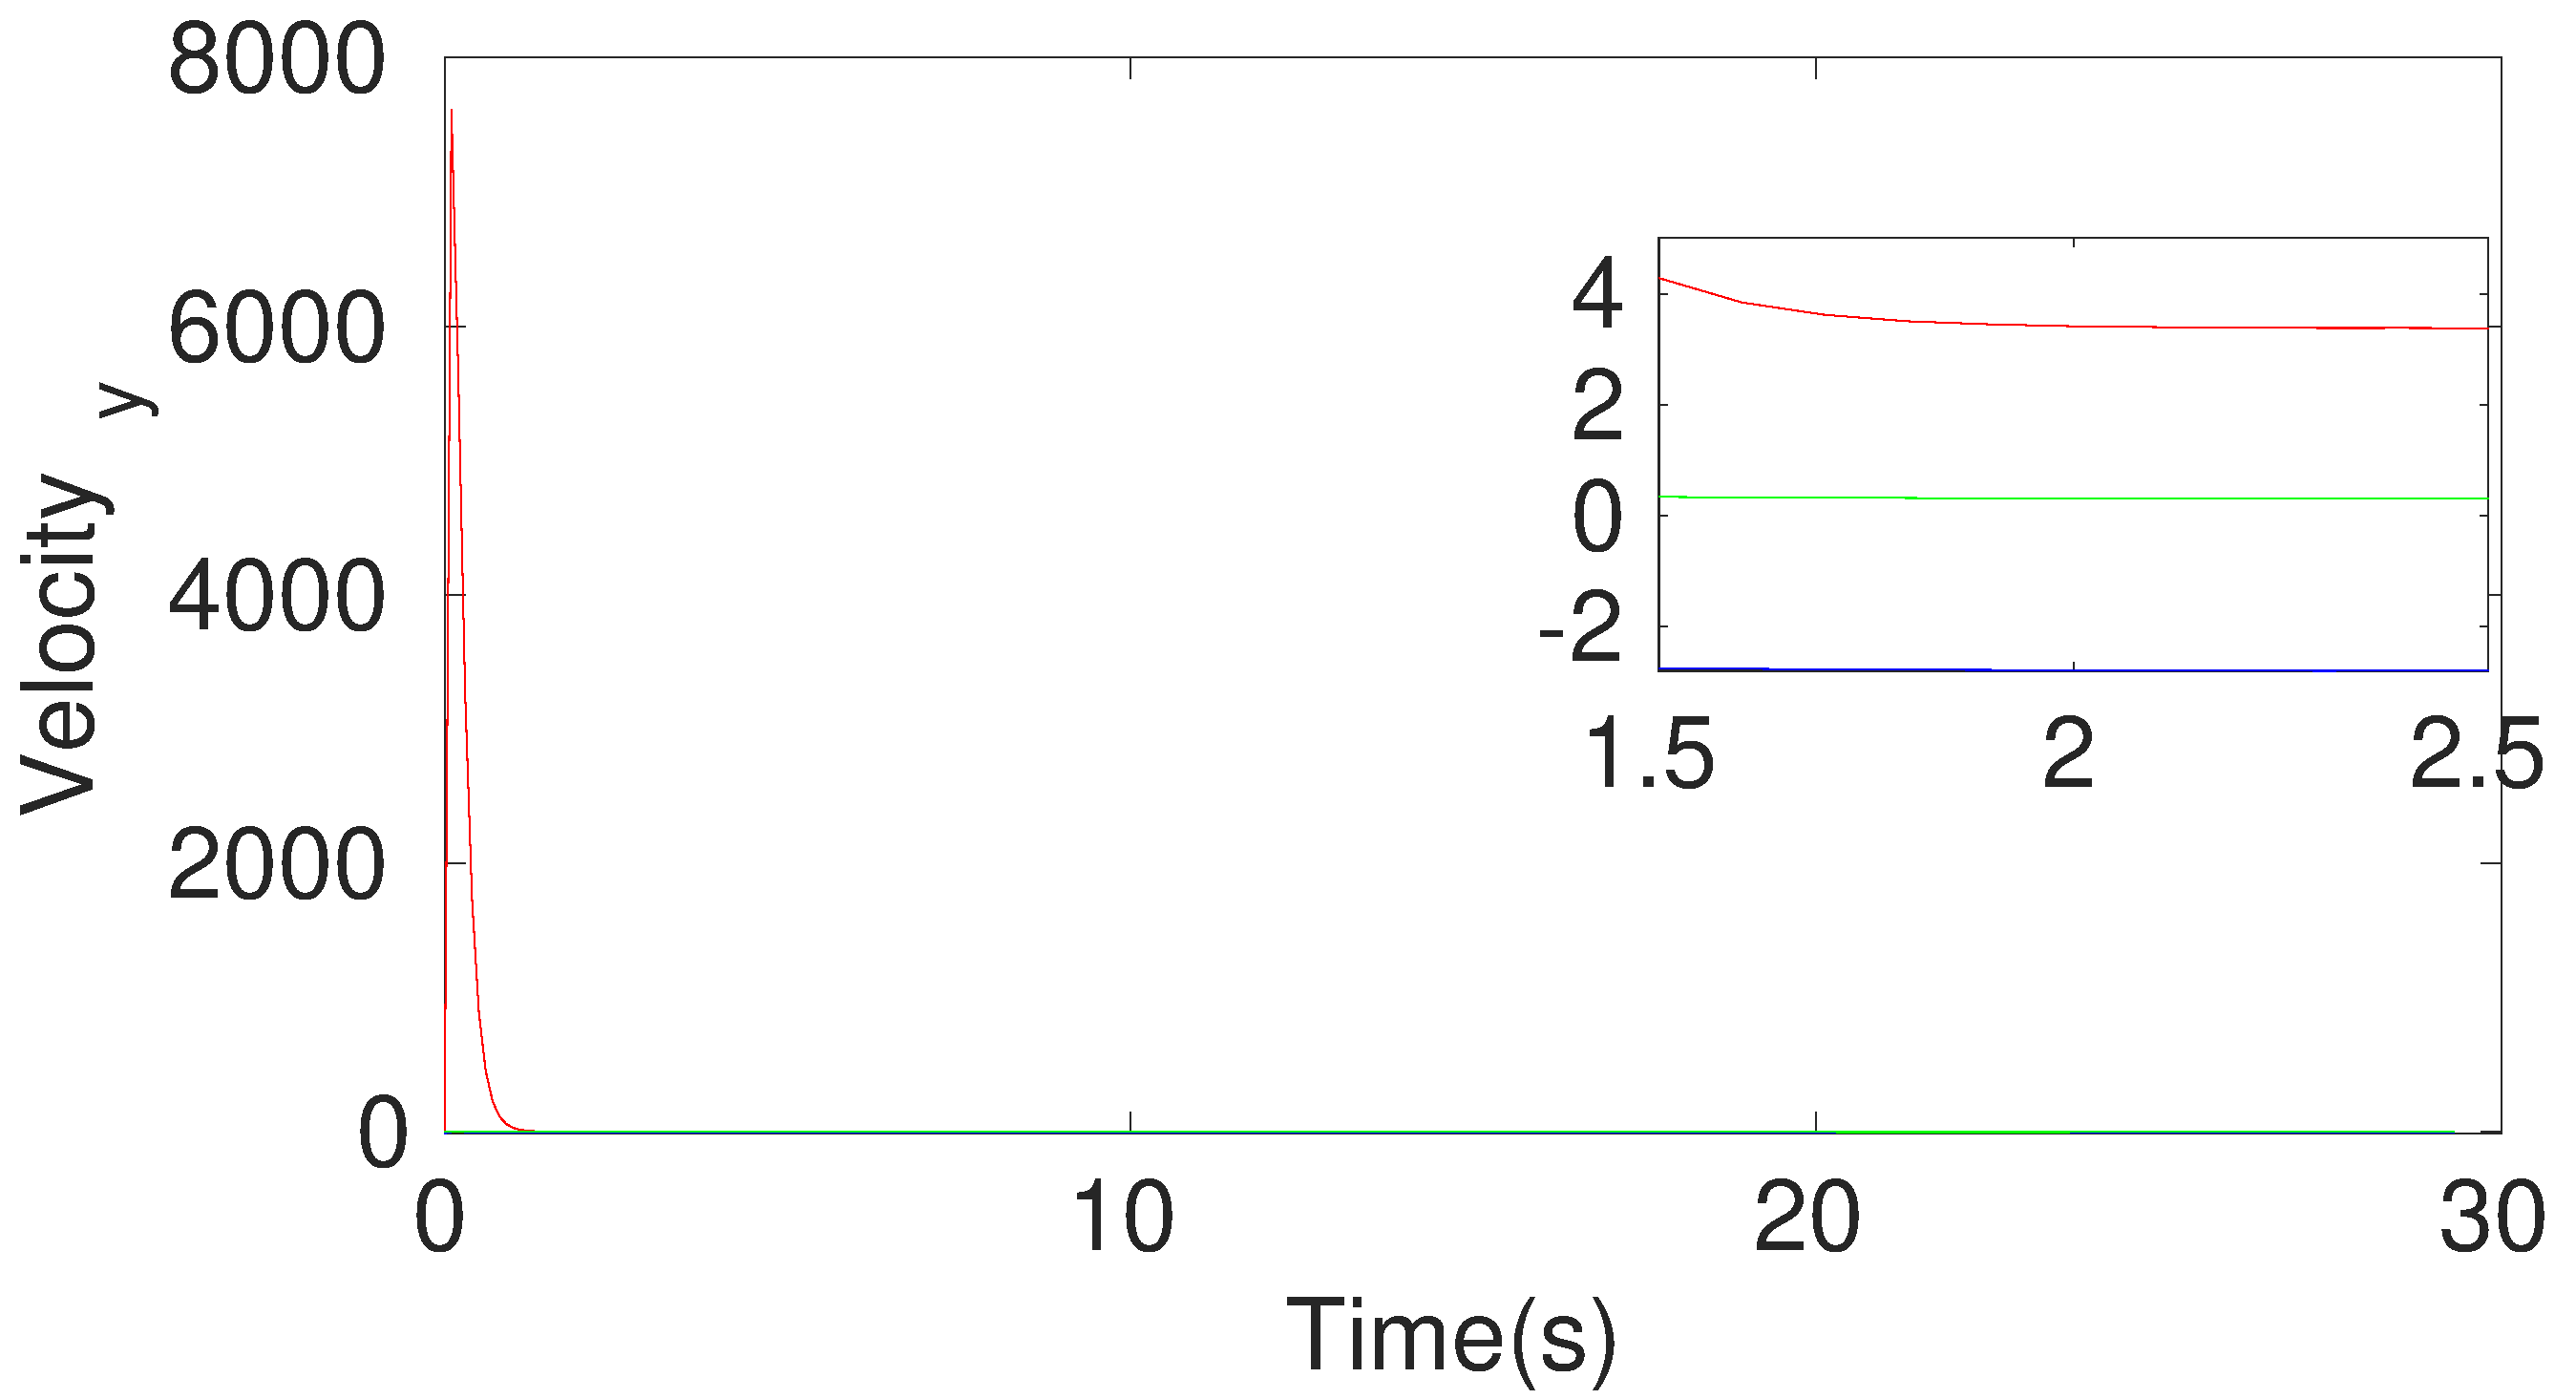
\includegraphics[width=.9\linewidth]{figures/HInf/s3cvHInfVelocity_y}
\end{subfigure}
\caption{Estimation using Constant Velocity}
\end{figure}

\begin{figure}[h]
\begin{subfigure}{.5\linewidth}
\centering
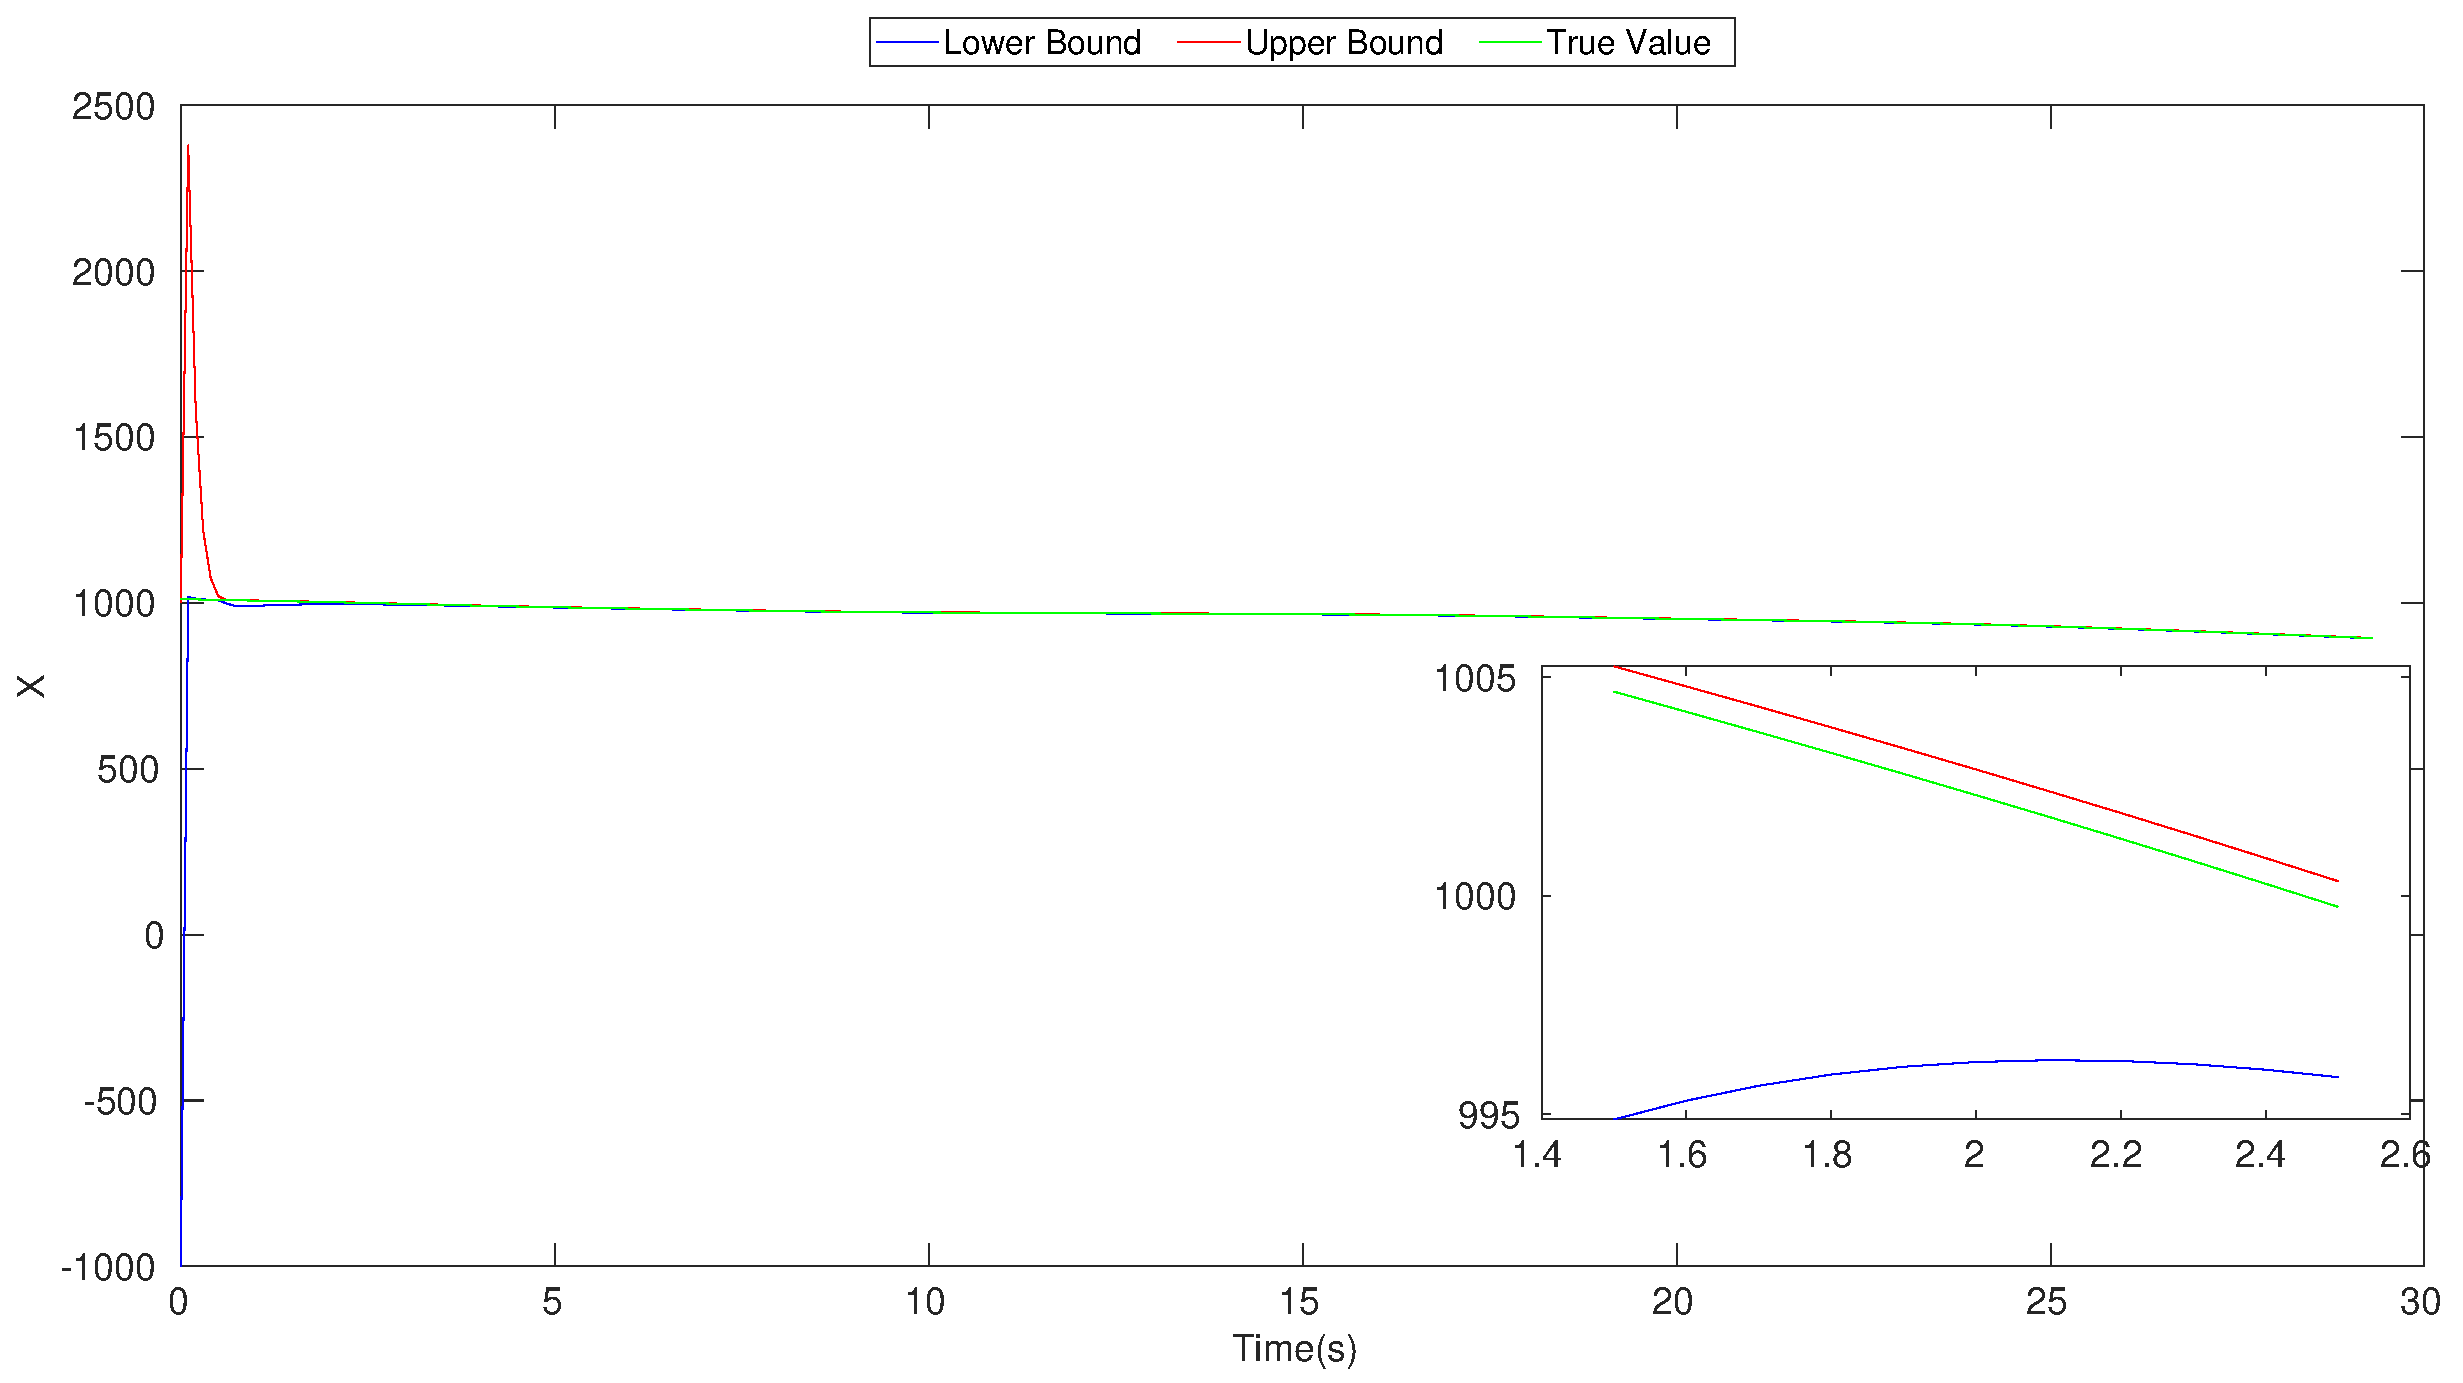
\includegraphics[width=\linewidth]{figures/HInf/s3caHInfX}
\end{subfigure}
\begin{subfigure}{.5\linewidth}
\centering
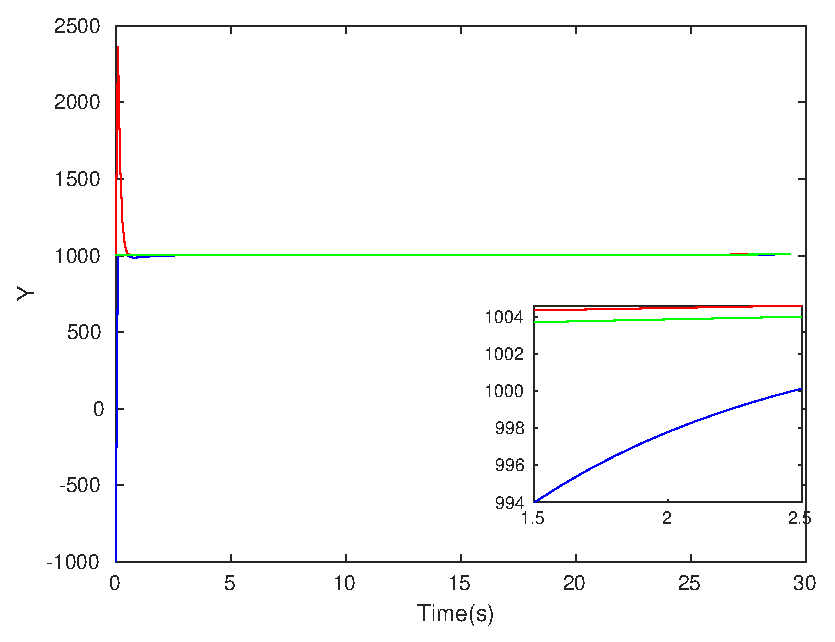
\includegraphics[width=\linewidth]{figures/HInf/s3caHInfY}
\end{subfigure}
\begin{subfigure}{.5\linewidth}
\centering
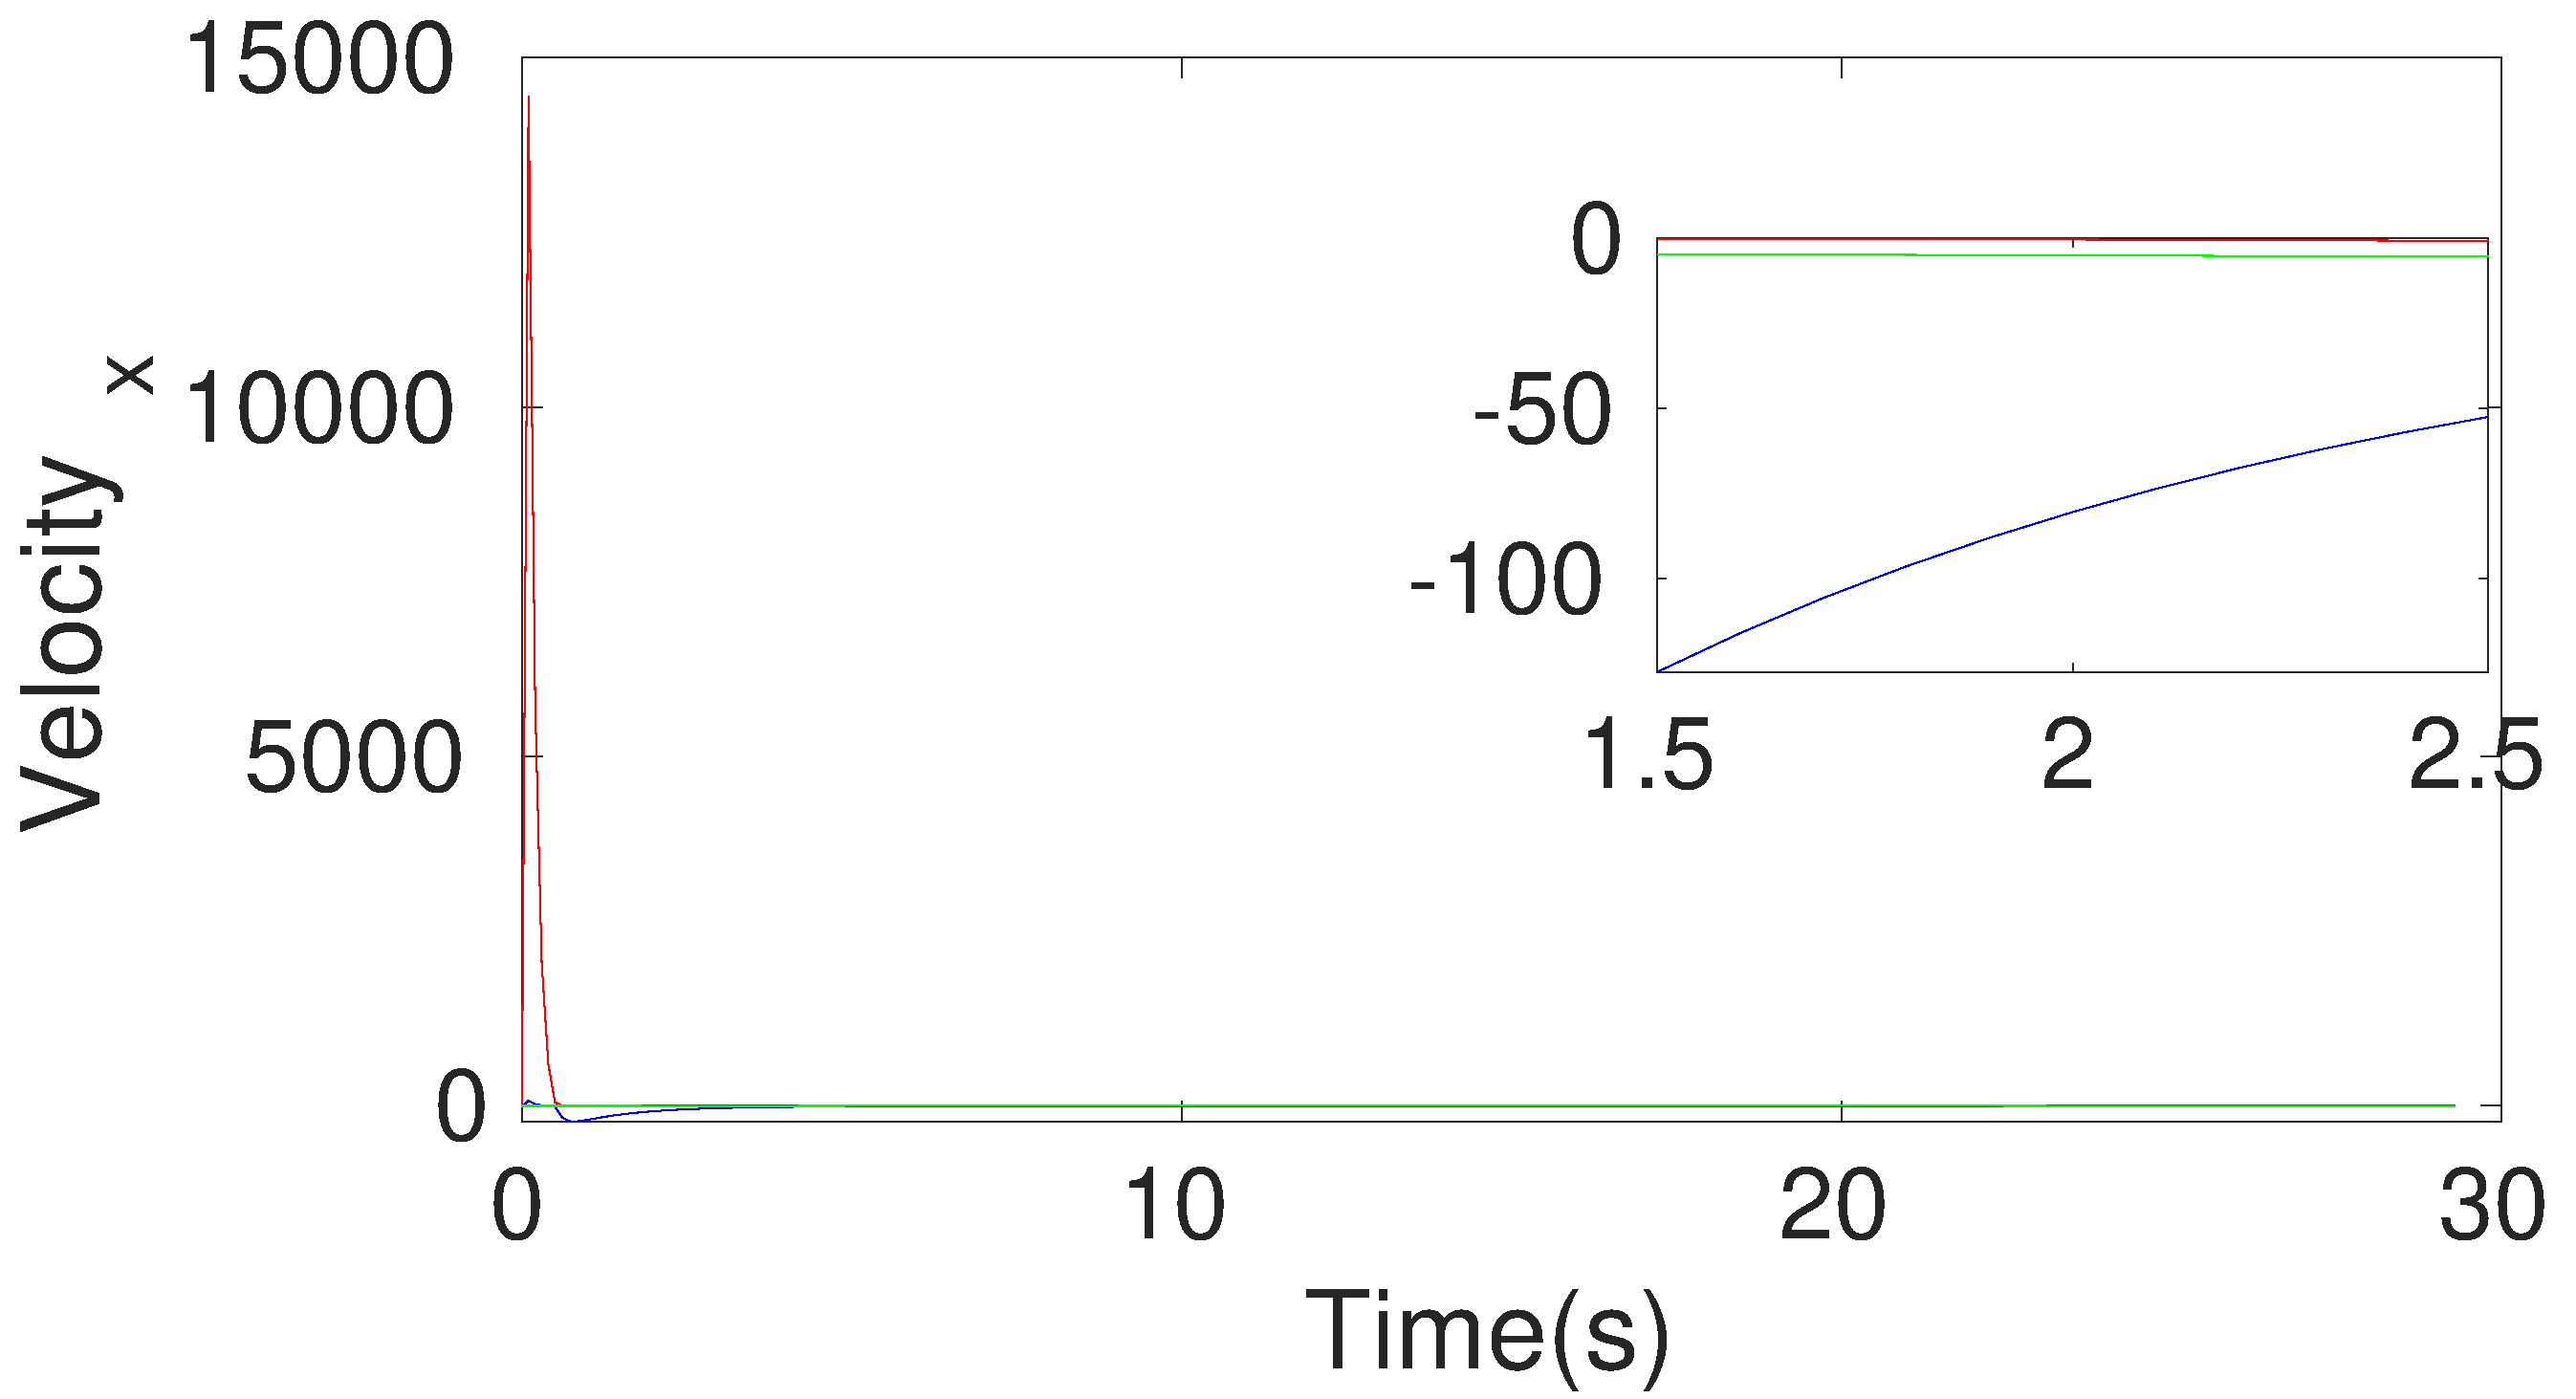
\includegraphics[width=.9\linewidth]{figures/HInf/s3caHInfVelocity_x}
\end{subfigure}
\begin{subfigure}{.5\linewidth}
\centering
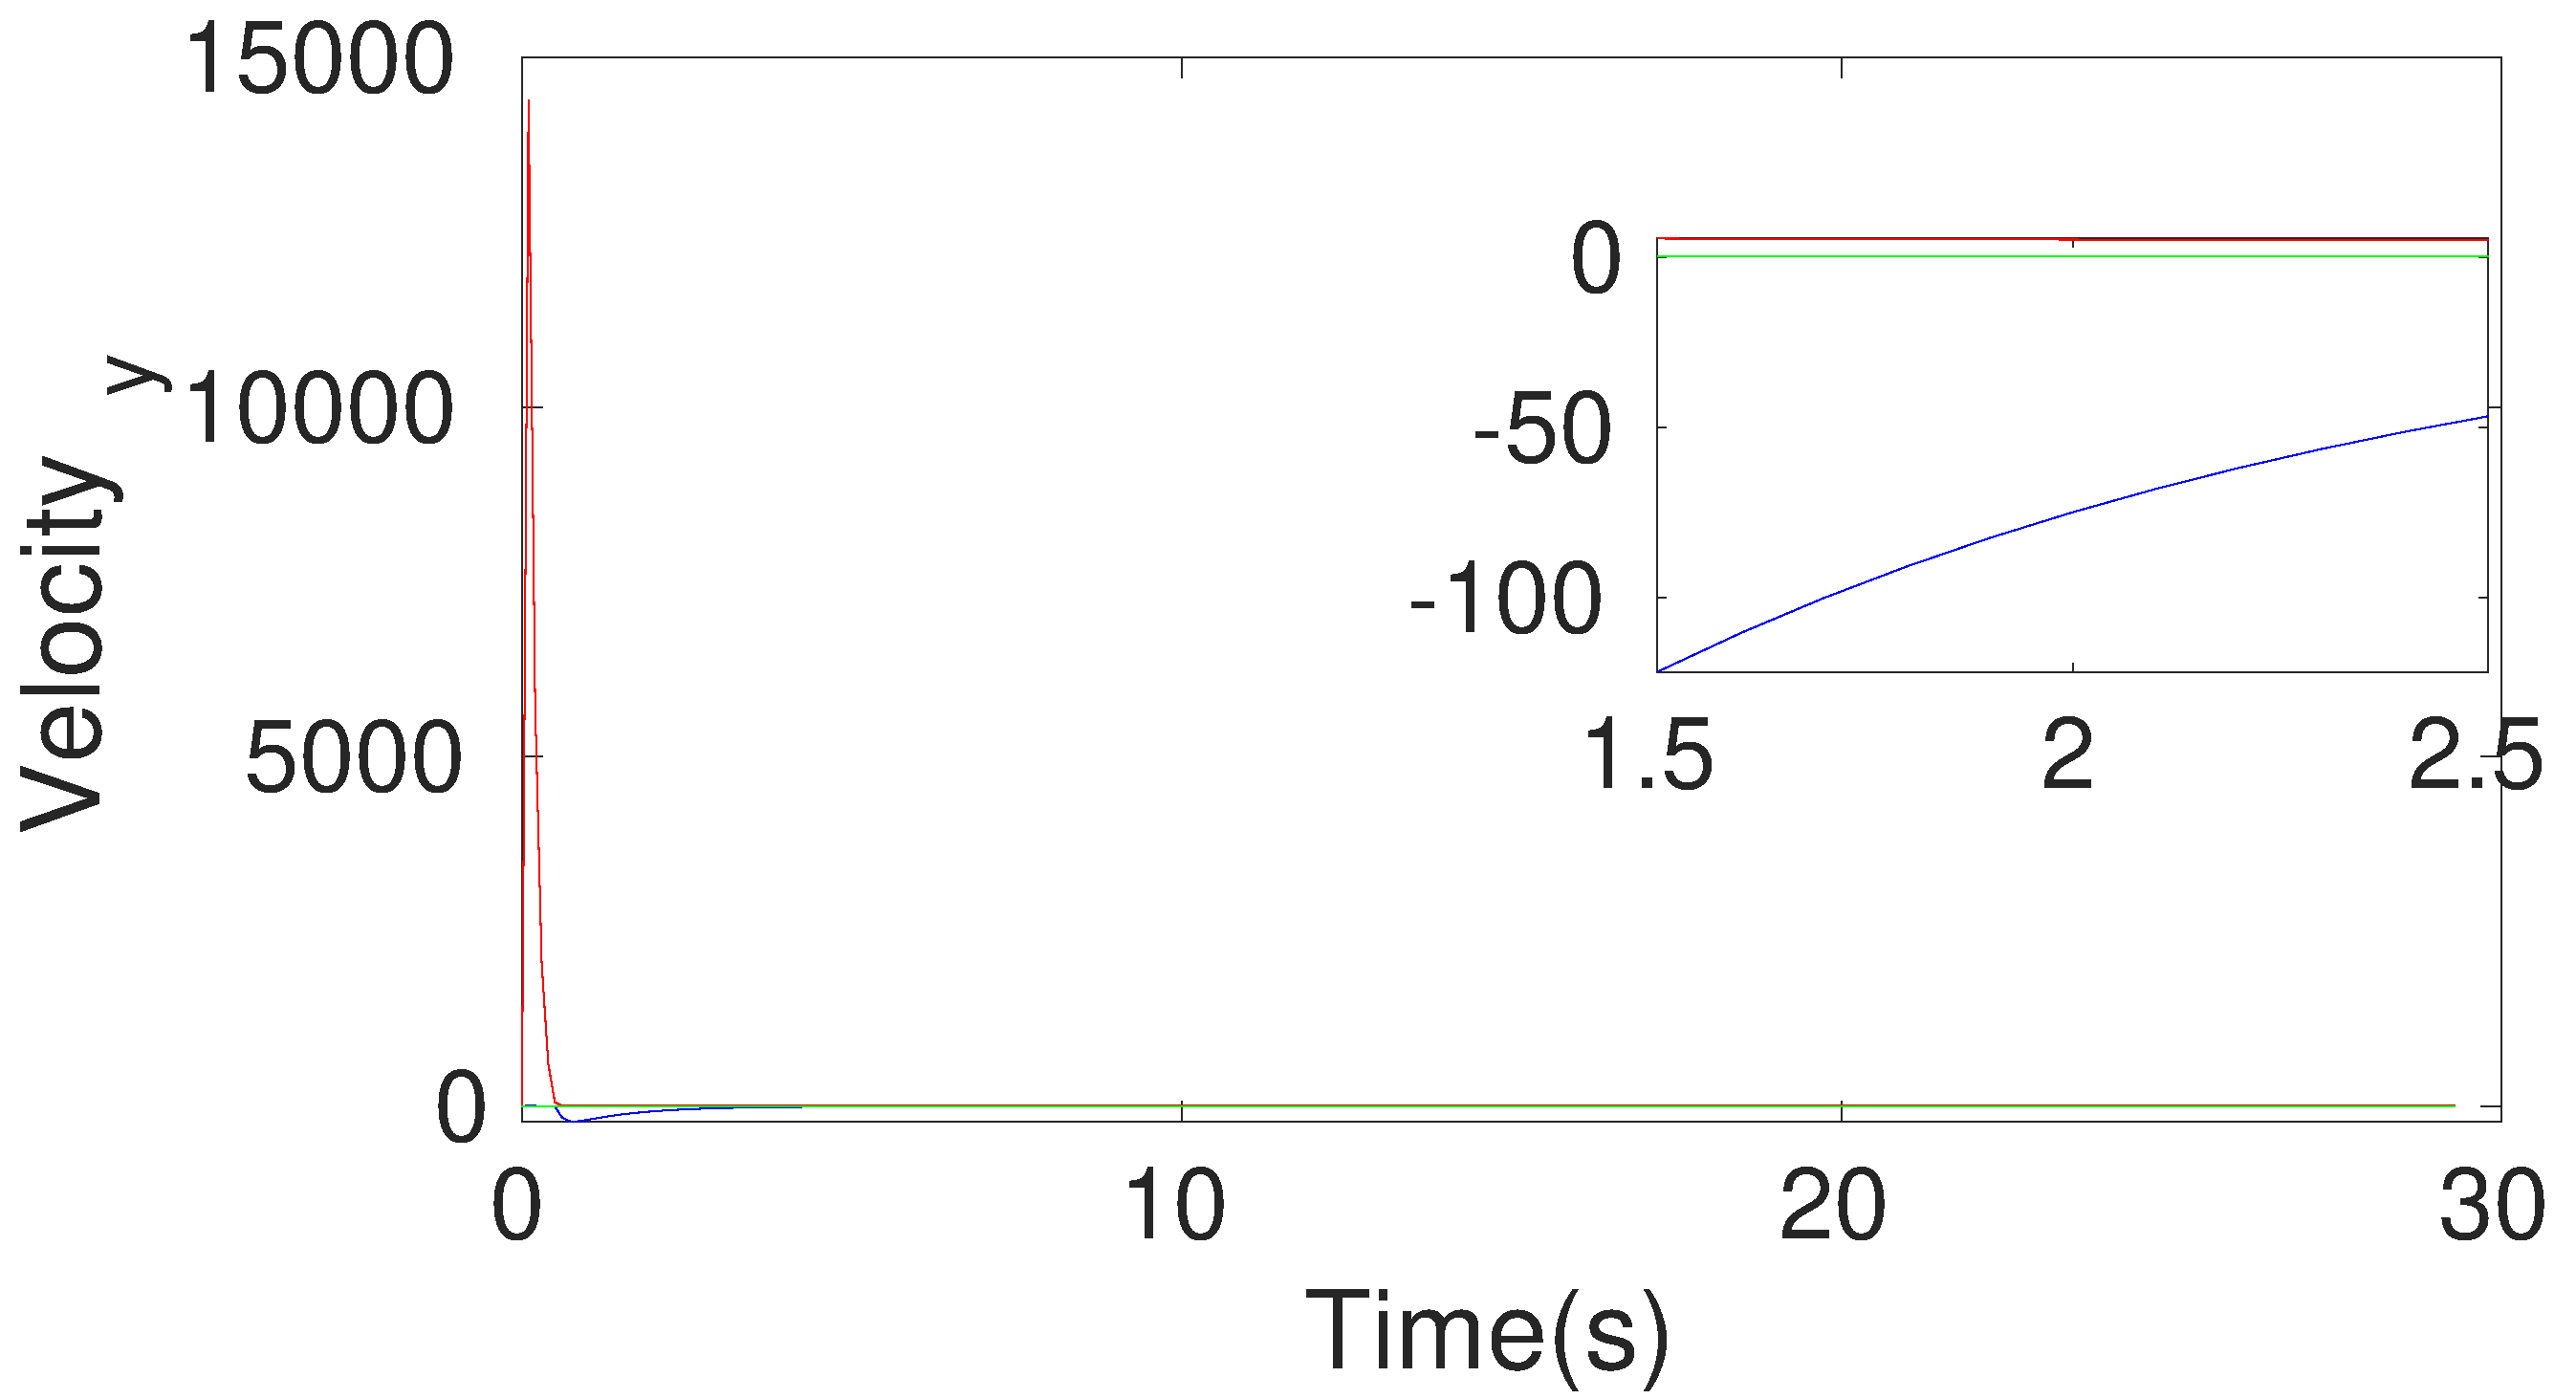
\includegraphics[width=.9\linewidth]{figures/HInf/s3caHInfVelocity_y}
\end{subfigure}
\begin{subfigure}{.5\linewidth}
\centering
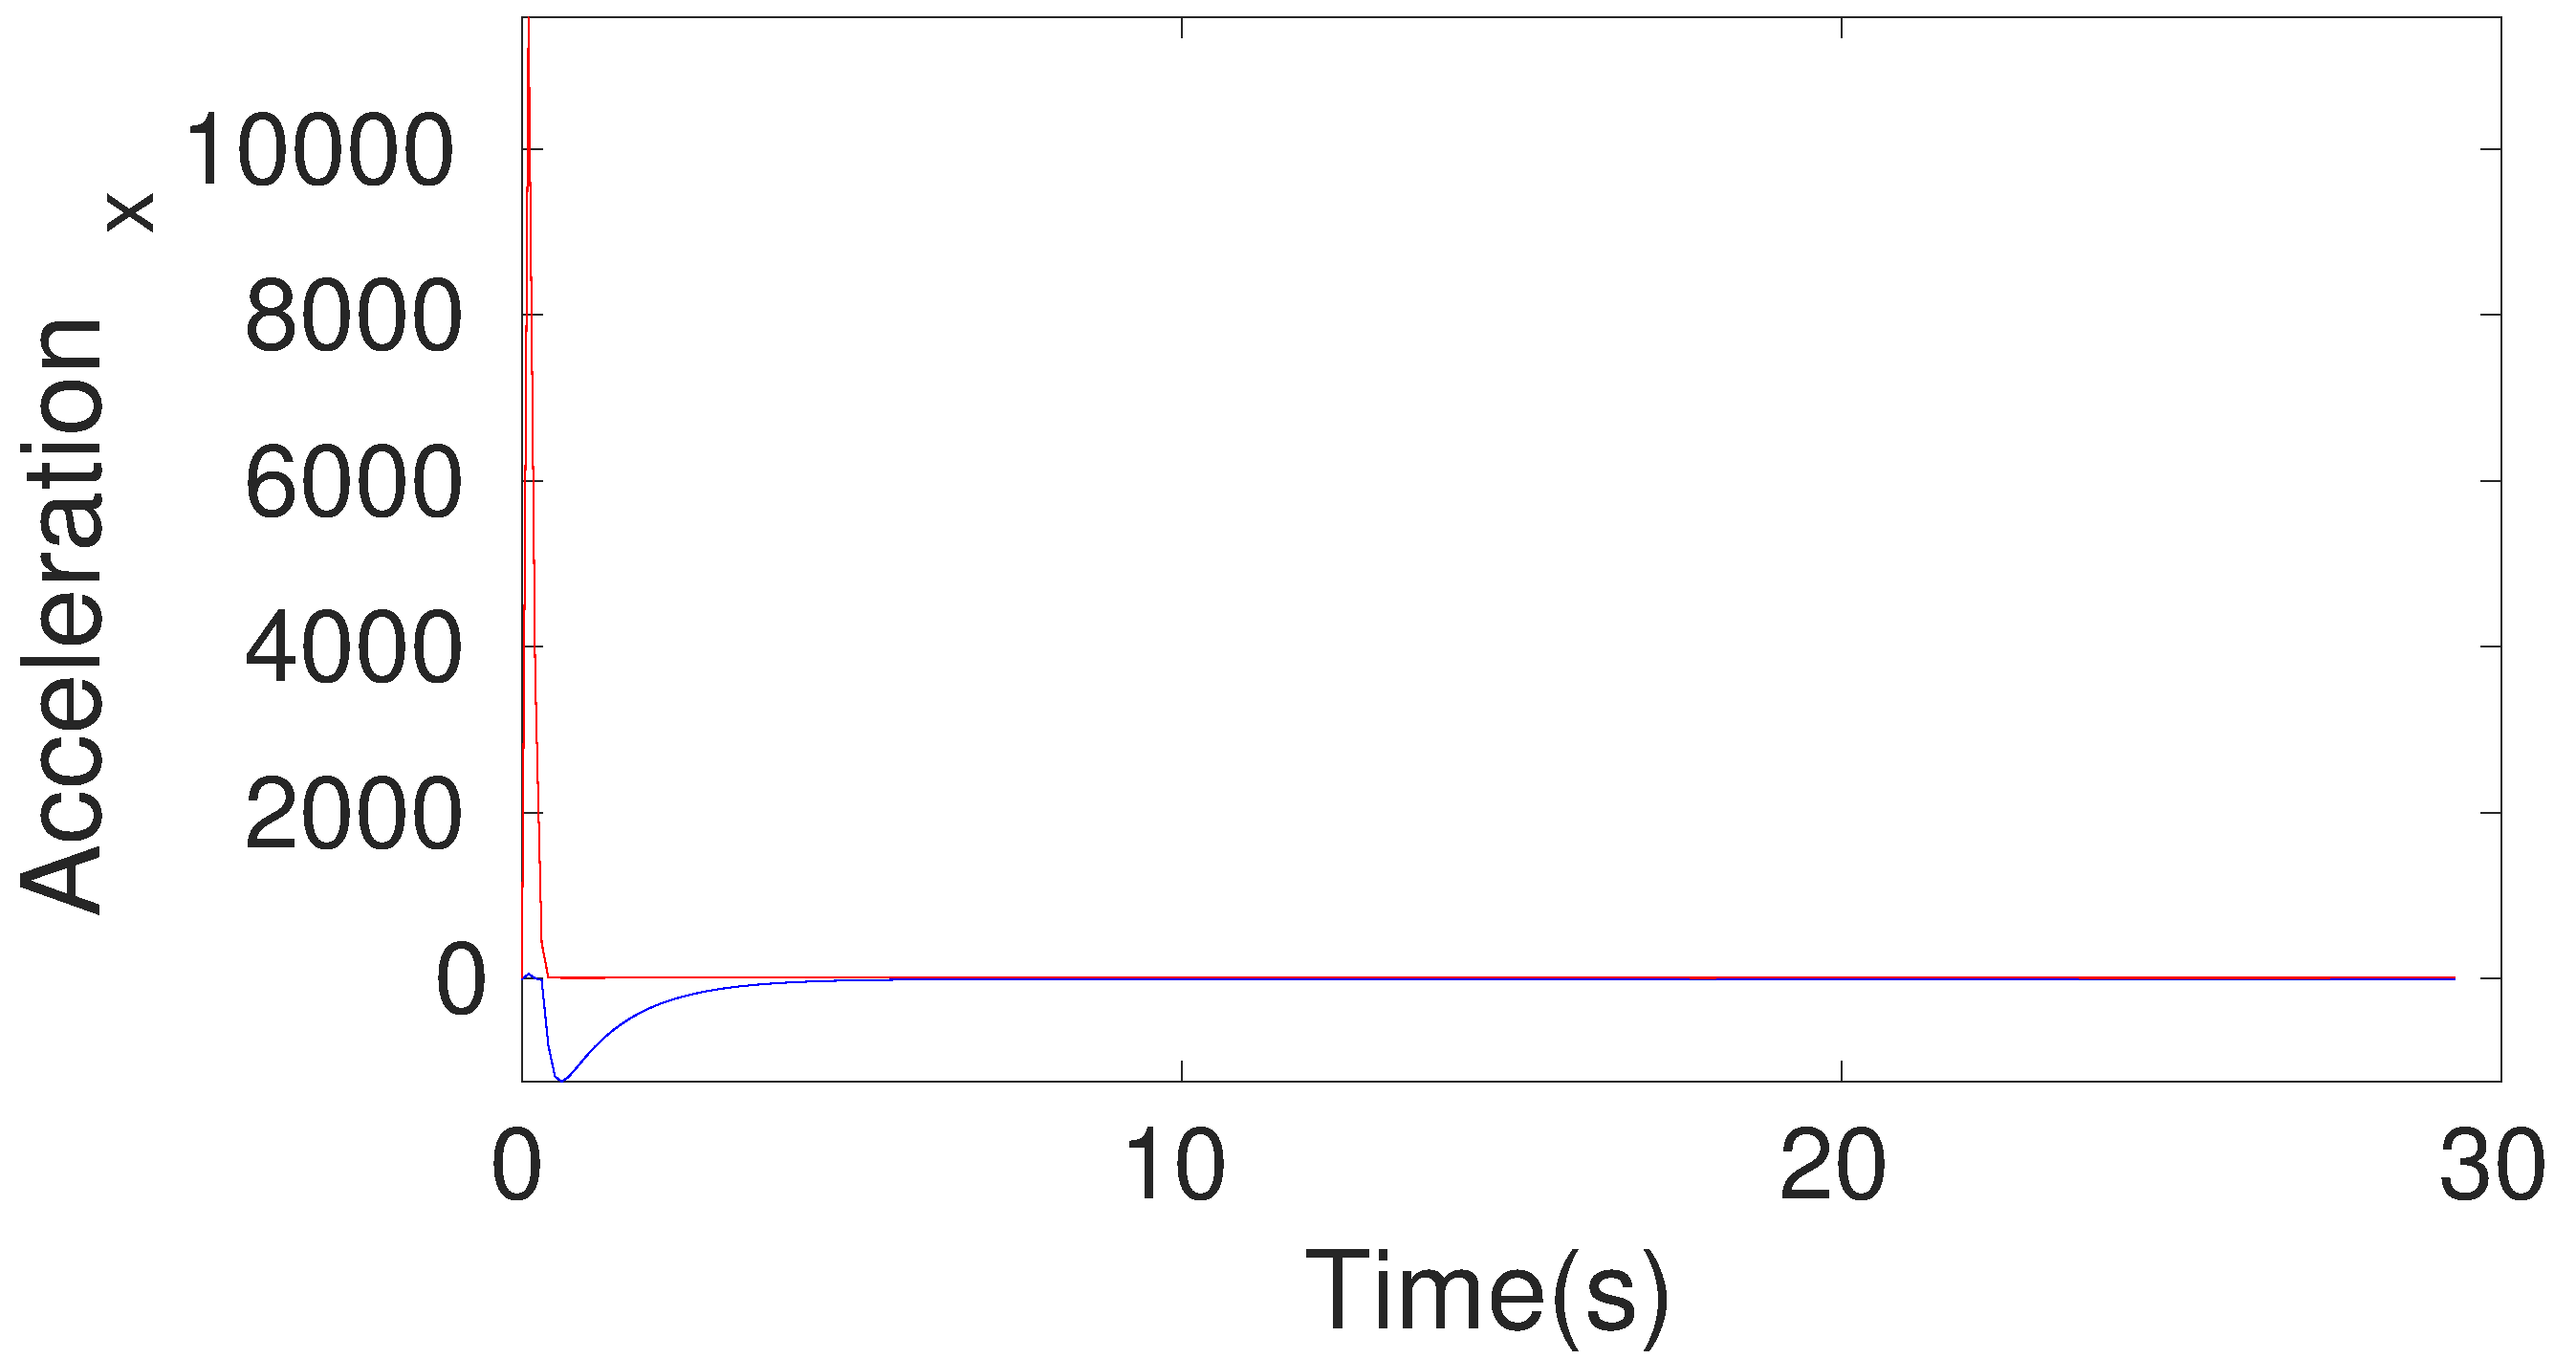
\includegraphics[width=.9\linewidth]{figures/HInf/s3caHInfAcceleration_x}
\end{subfigure}
\begin{subfigure}{.5\linewidth}
\centering
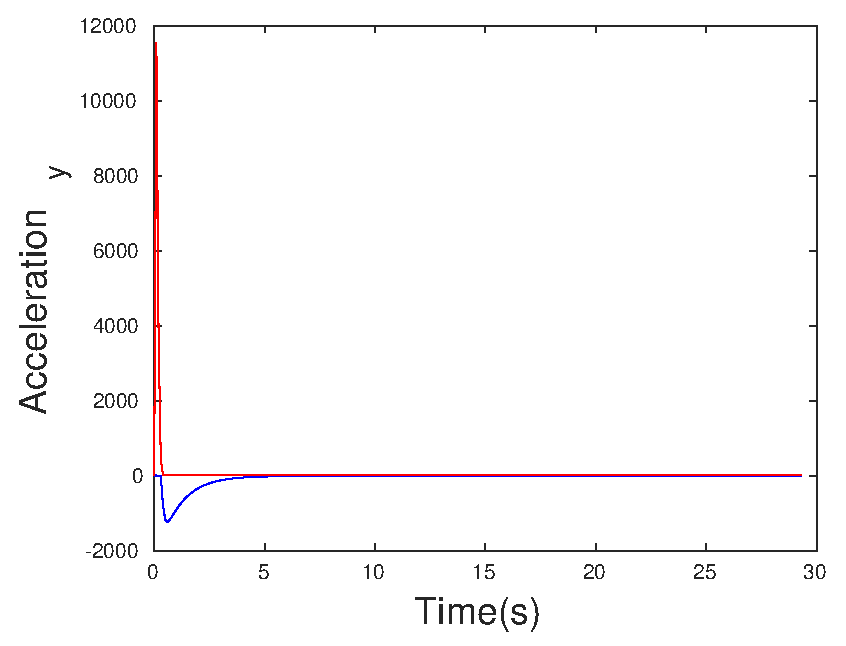
\includegraphics[width=.9\linewidth]{figures/HInf/s3caHInfAcceleration_y}
\end{subfigure}
\caption{Estimation using Constant Acceleration}
\end{figure}



\begin{figure}[h]
\begin{subfigure}{.5\linewidth}
\centering
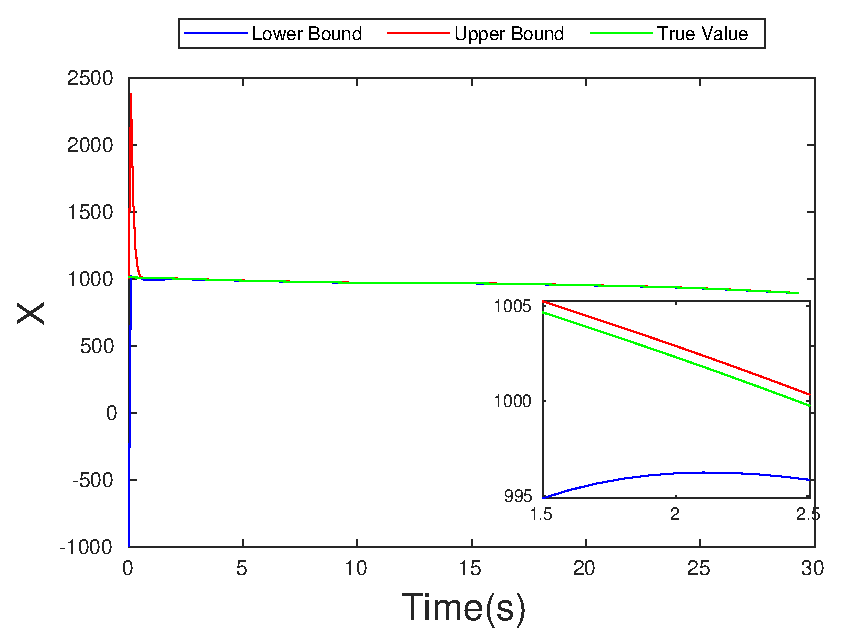
\includegraphics[width=\linewidth]{figures/HInf/s3pmHInfX}
\end{subfigure}
\begin{subfigure}{.5\linewidth}
\centering
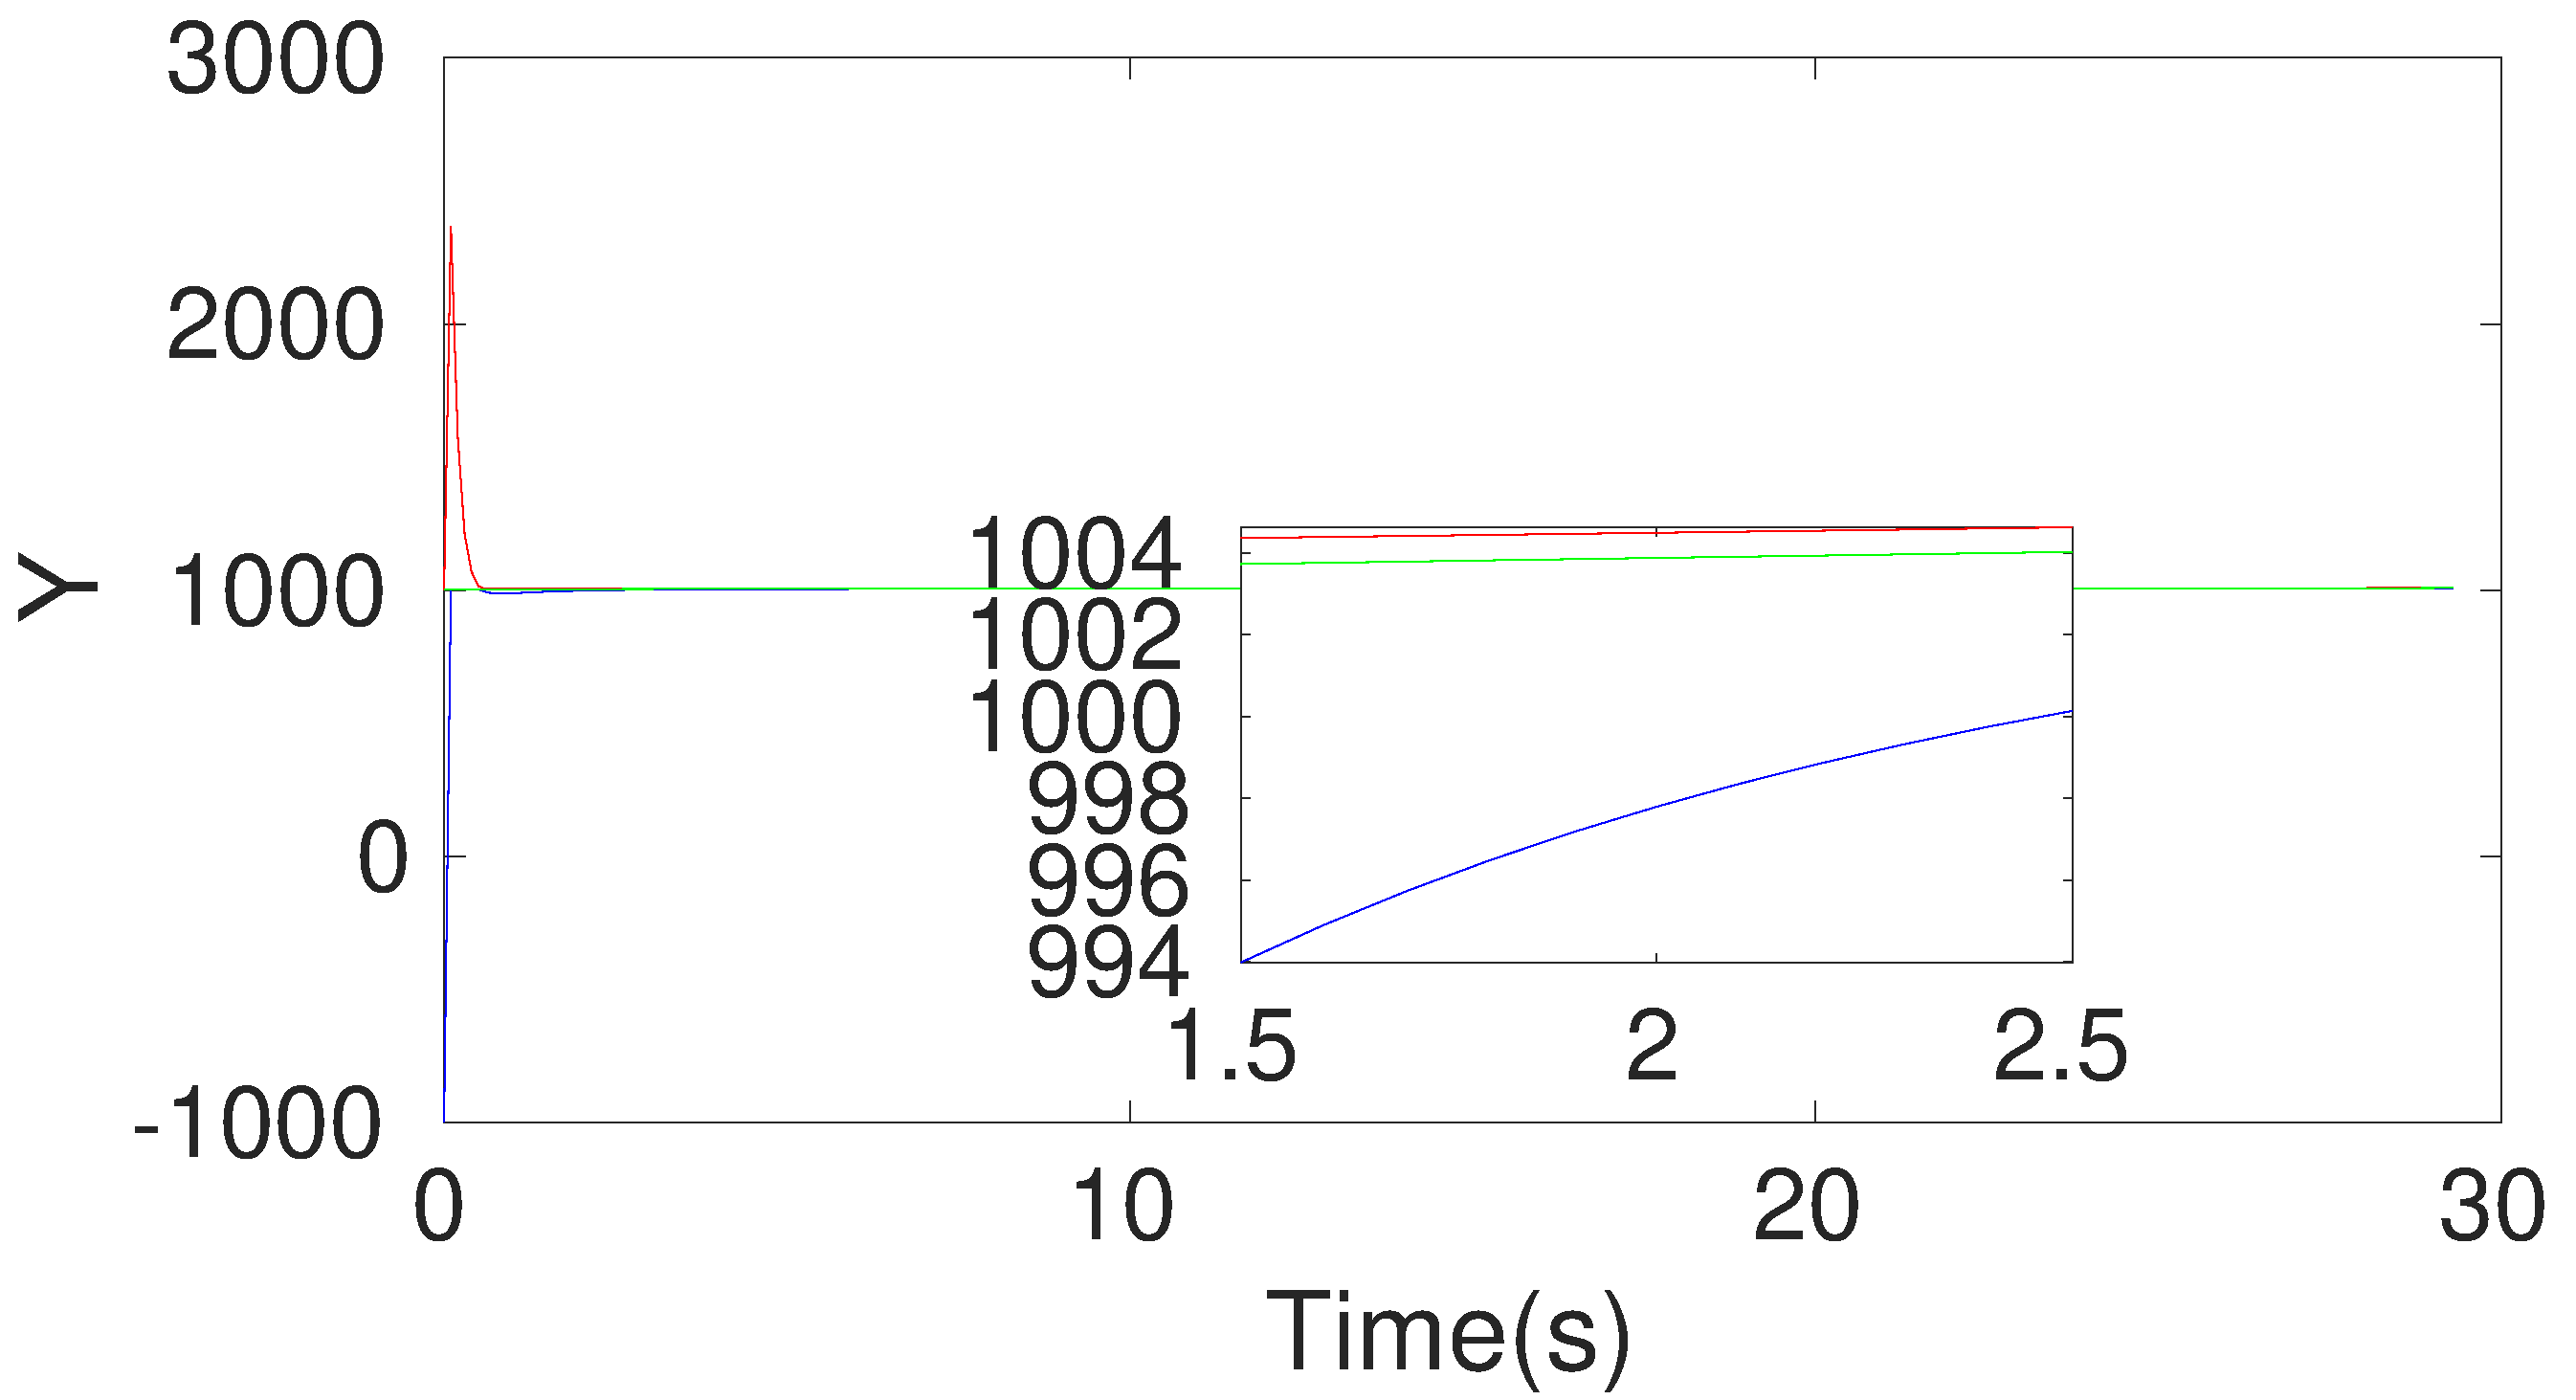
\includegraphics[width=\linewidth]{figures/HInf/s3pmHInfY}
\end{subfigure}
\begin{subfigure}{.5\linewidth}
\centering
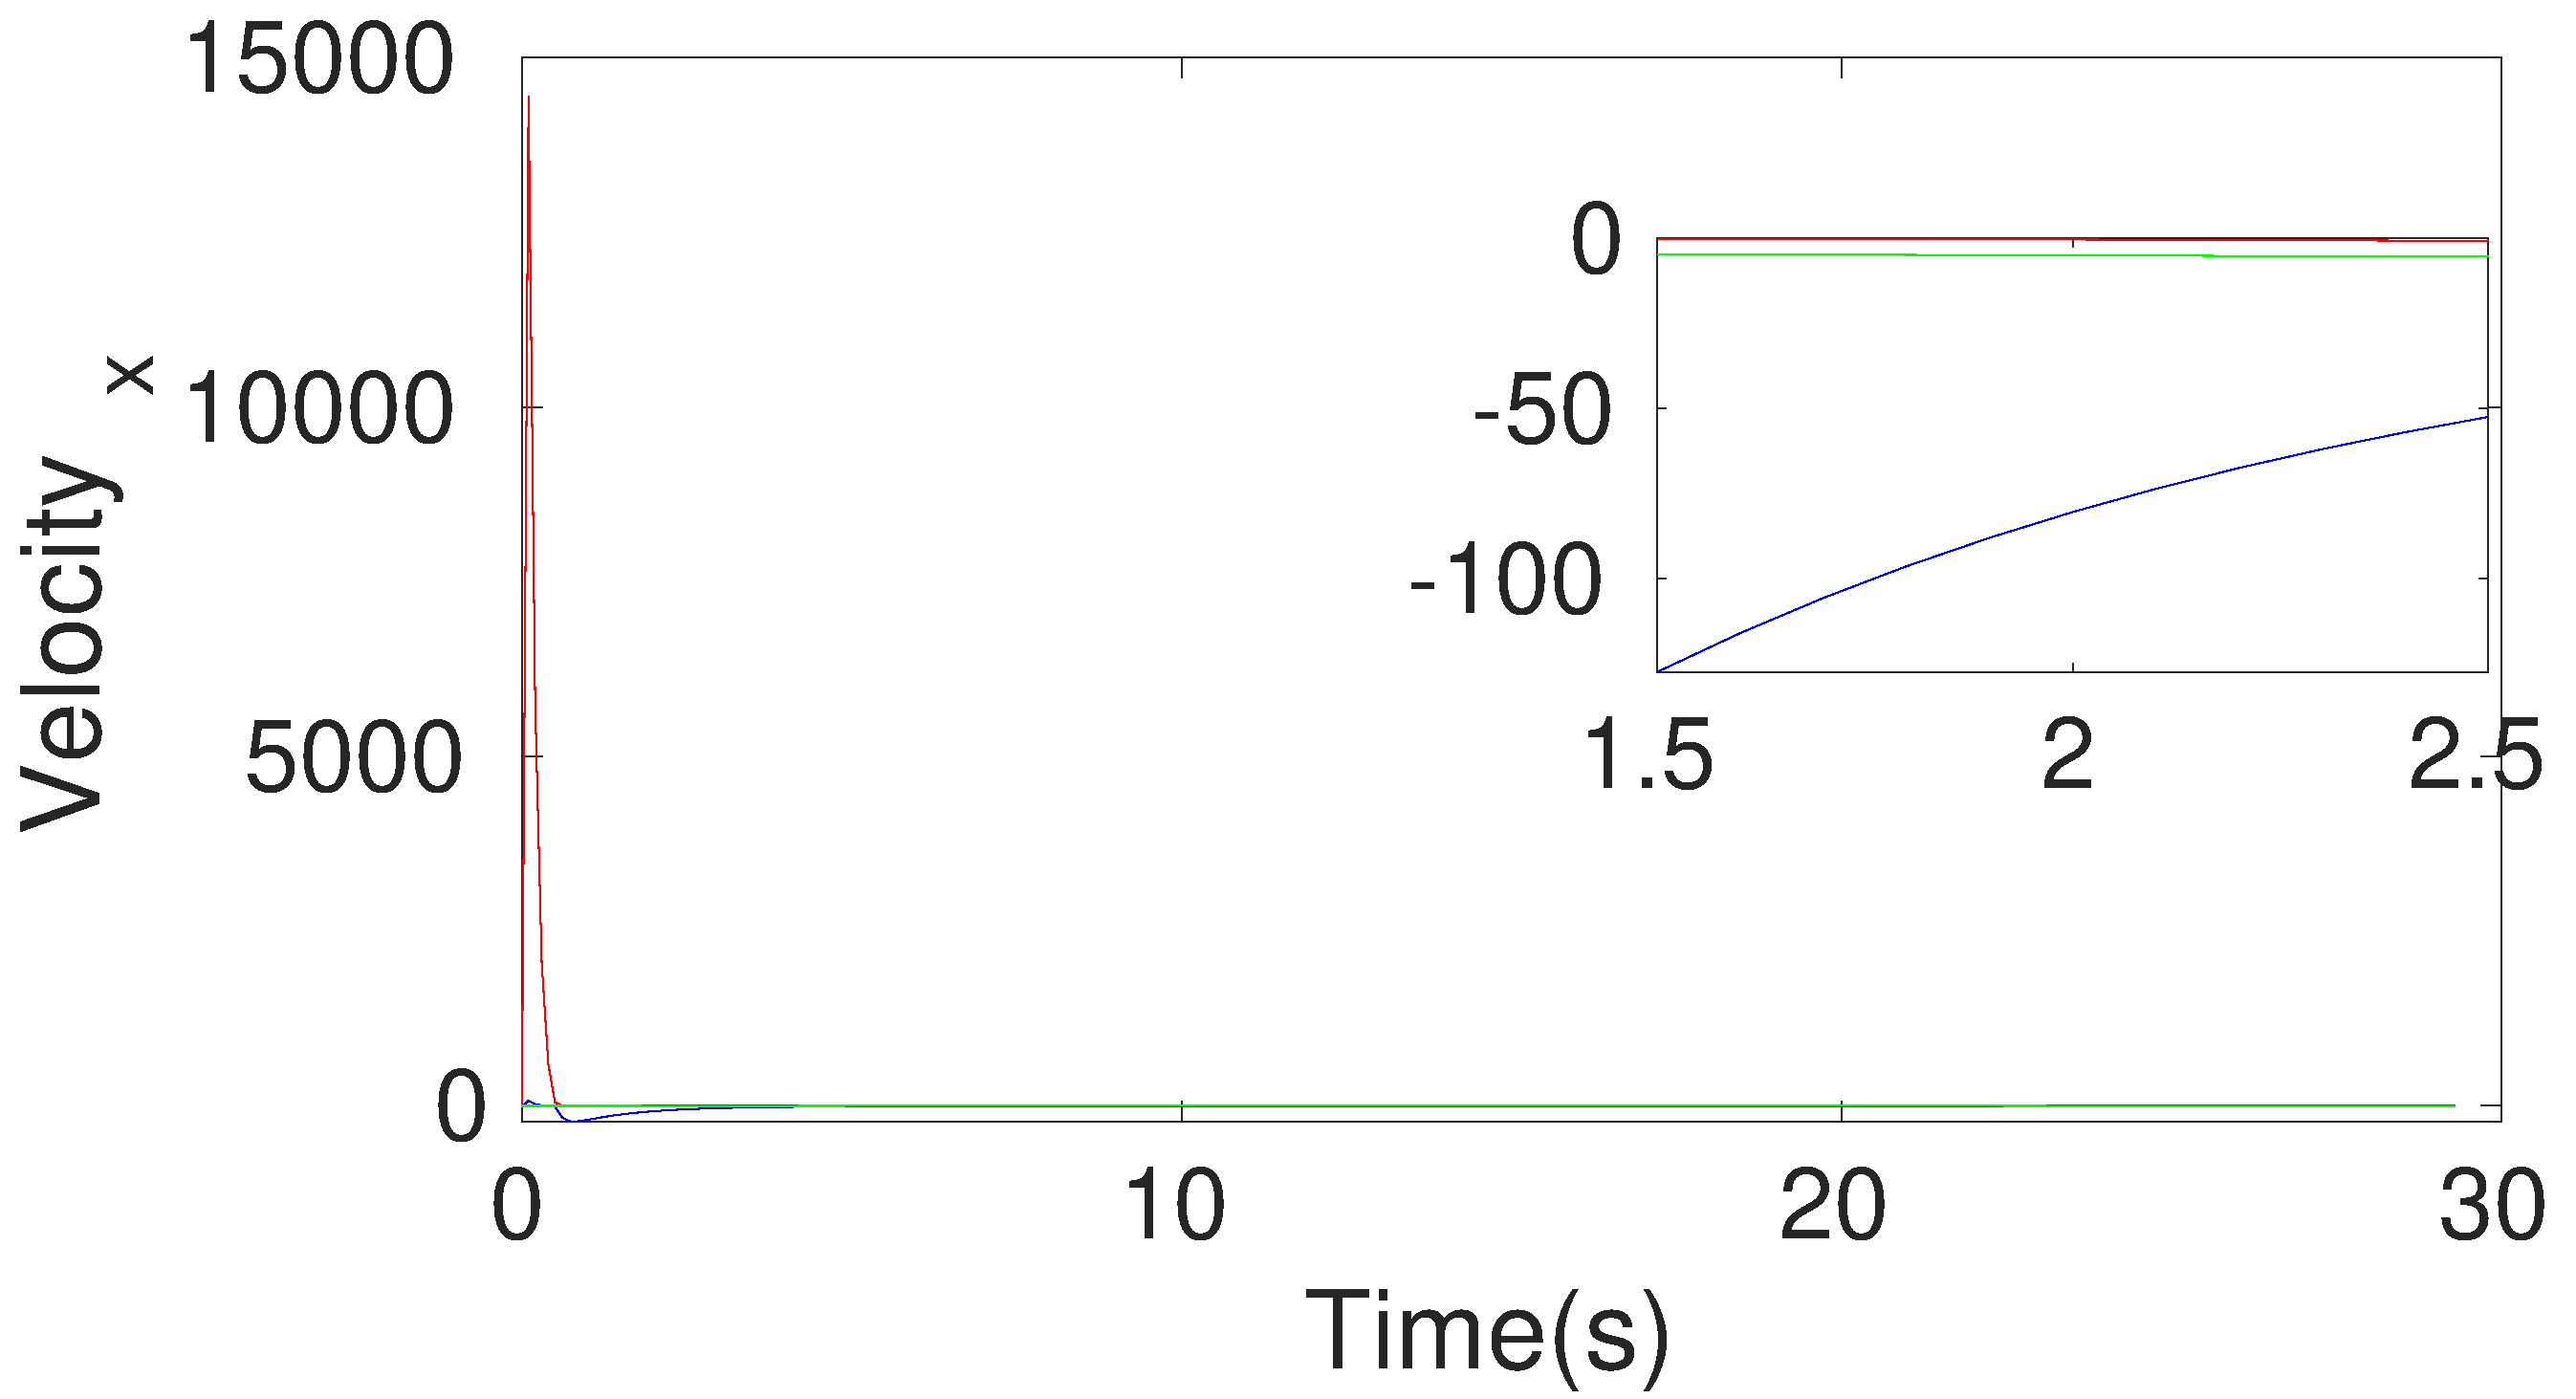
\includegraphics[width=.9\linewidth]{figures/HInf/s3pmHInfVelocity_x}
\end{subfigure}
\begin{subfigure}{.5\linewidth}
\centering
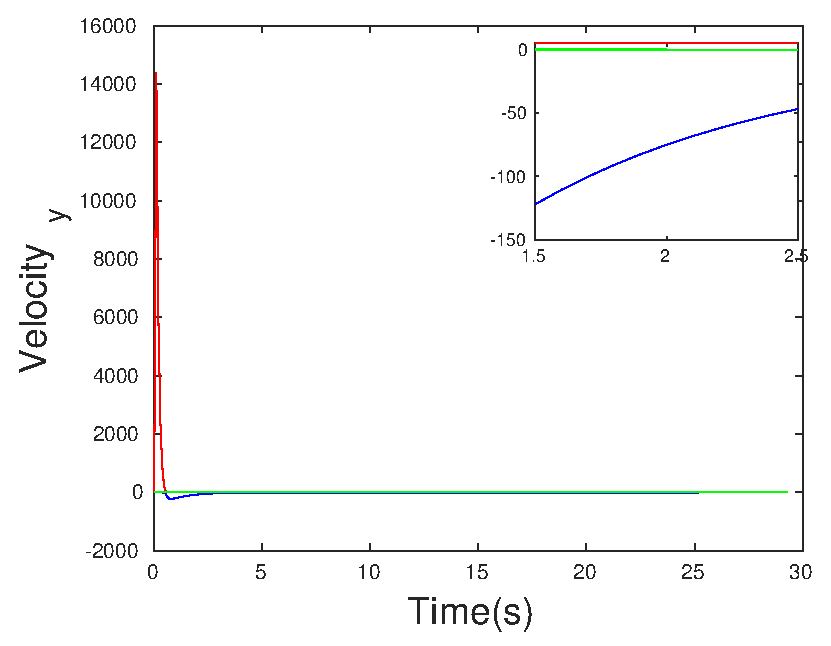
\includegraphics[width=.9\linewidth]{figures/HInf/s3pmHInfVelocity_y}
\end{subfigure}
\begin{subfigure}{.5\linewidth}
\centering
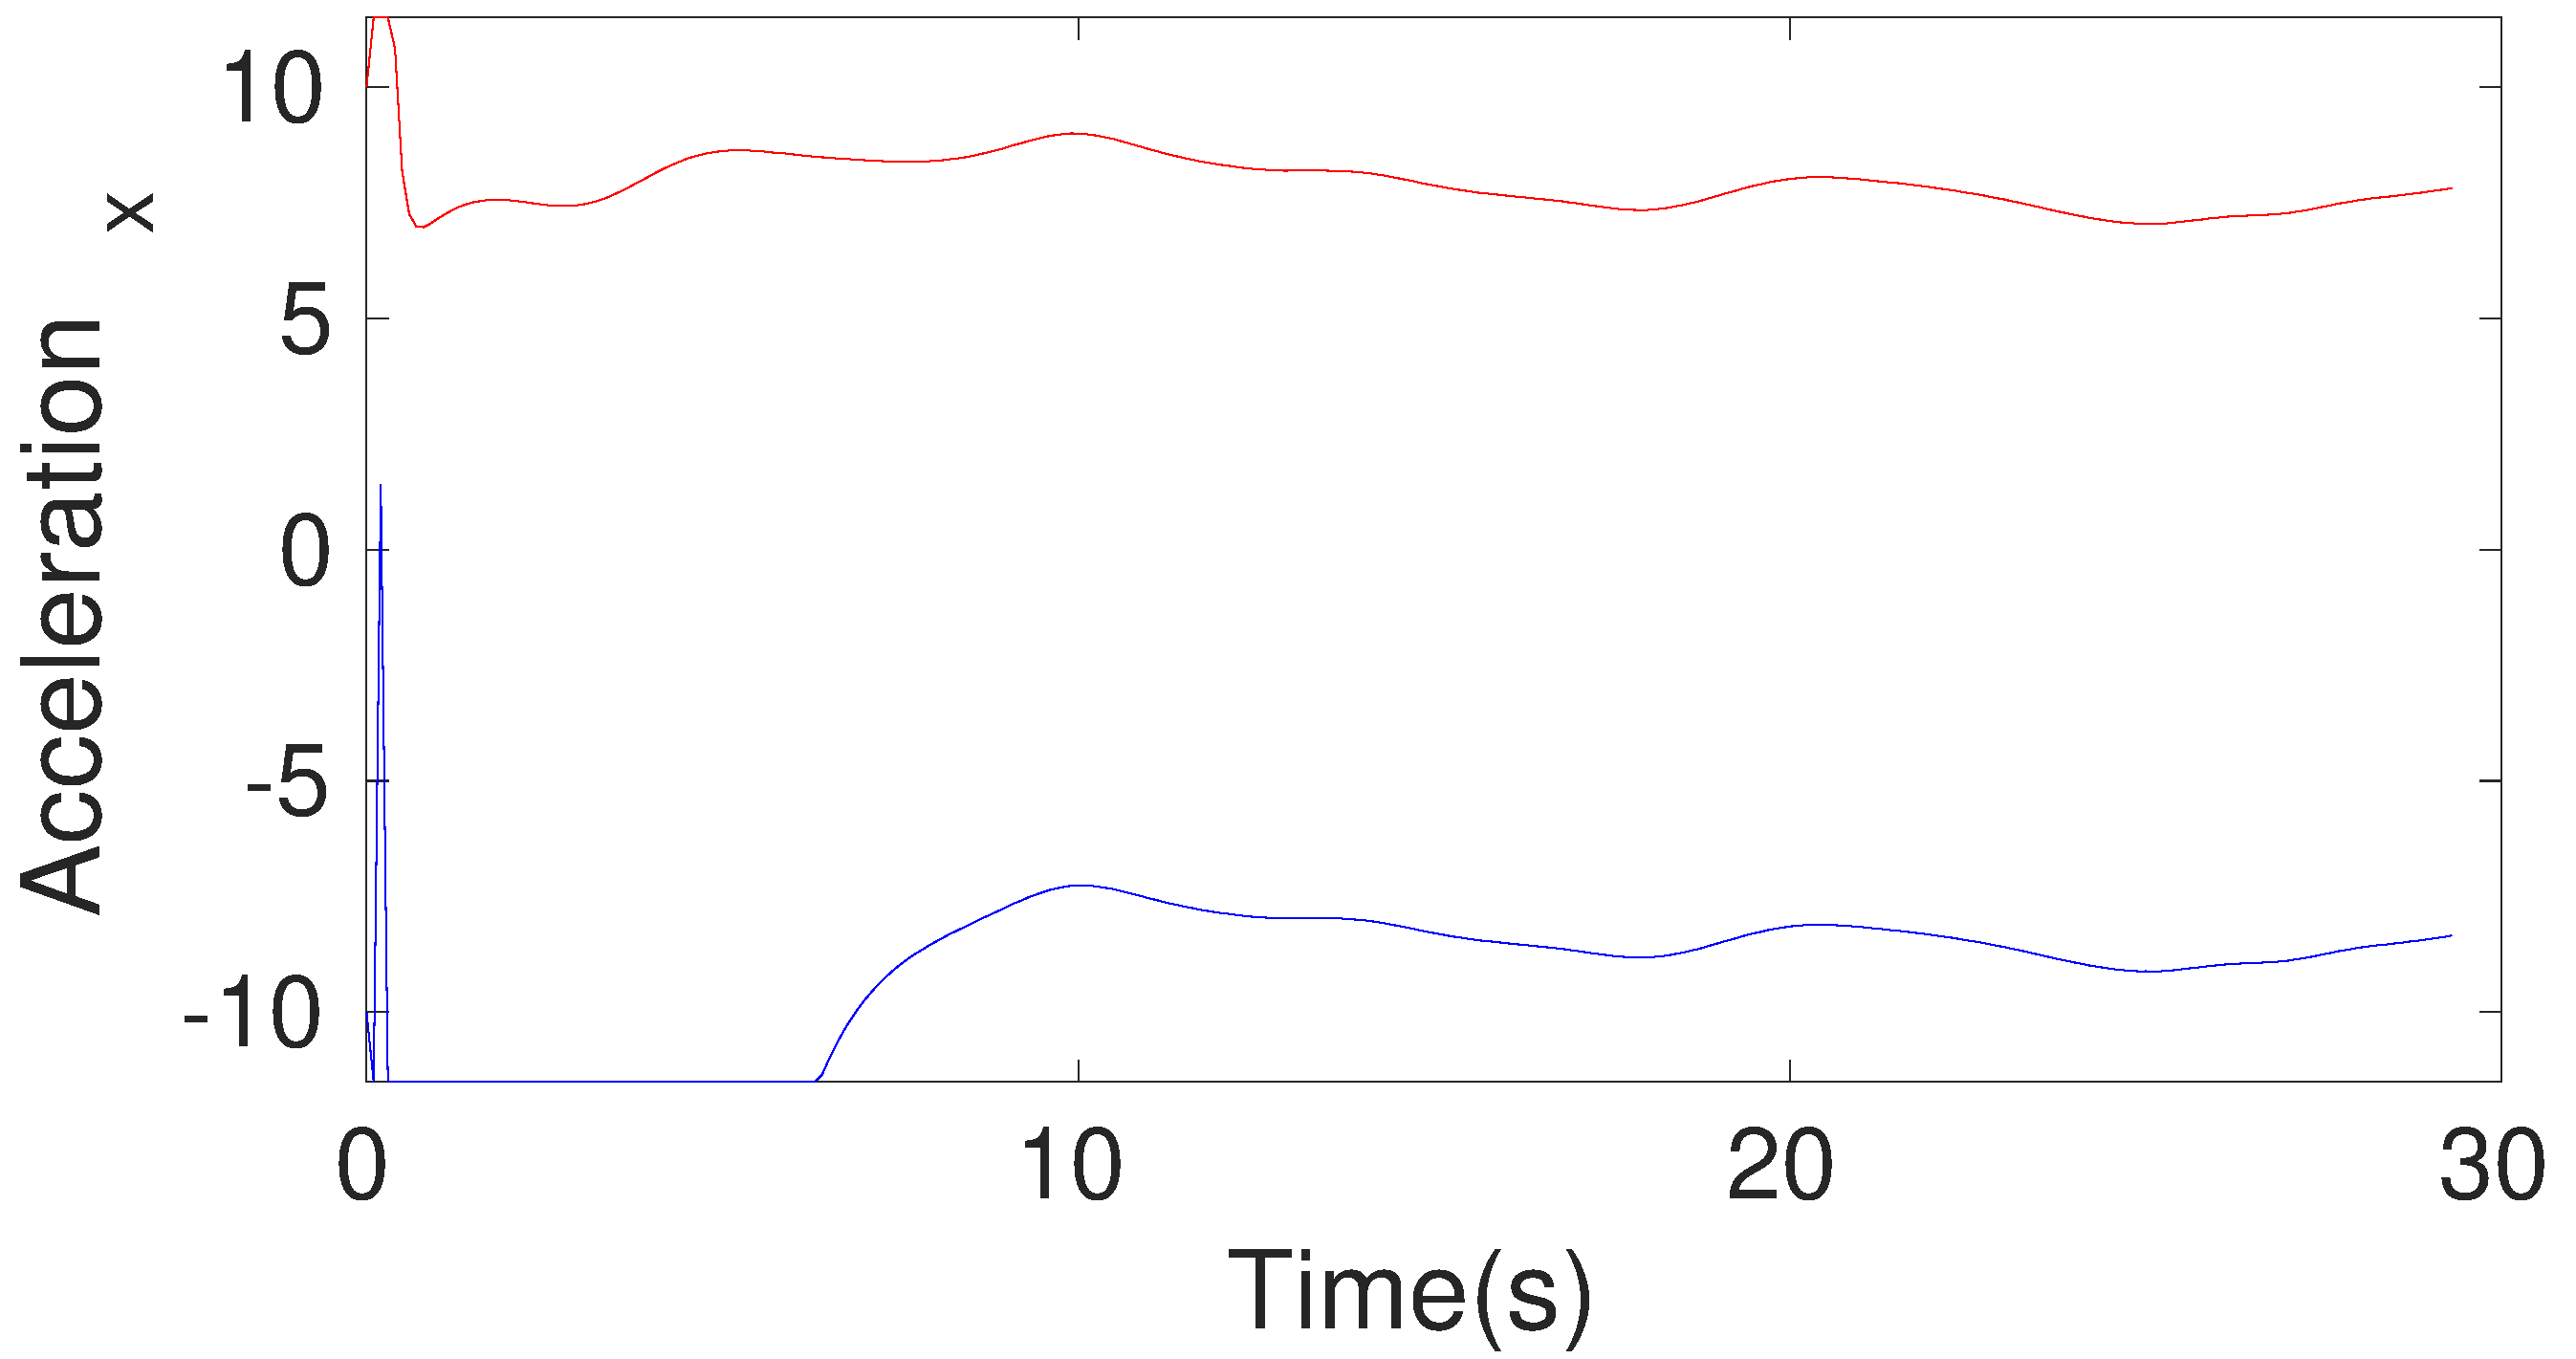
\includegraphics[width=.9\linewidth]{figures/HInf/s3pmHInfAcceleration_x}
\end{subfigure}
\begin{subfigure}{.5\linewidth}
\centering
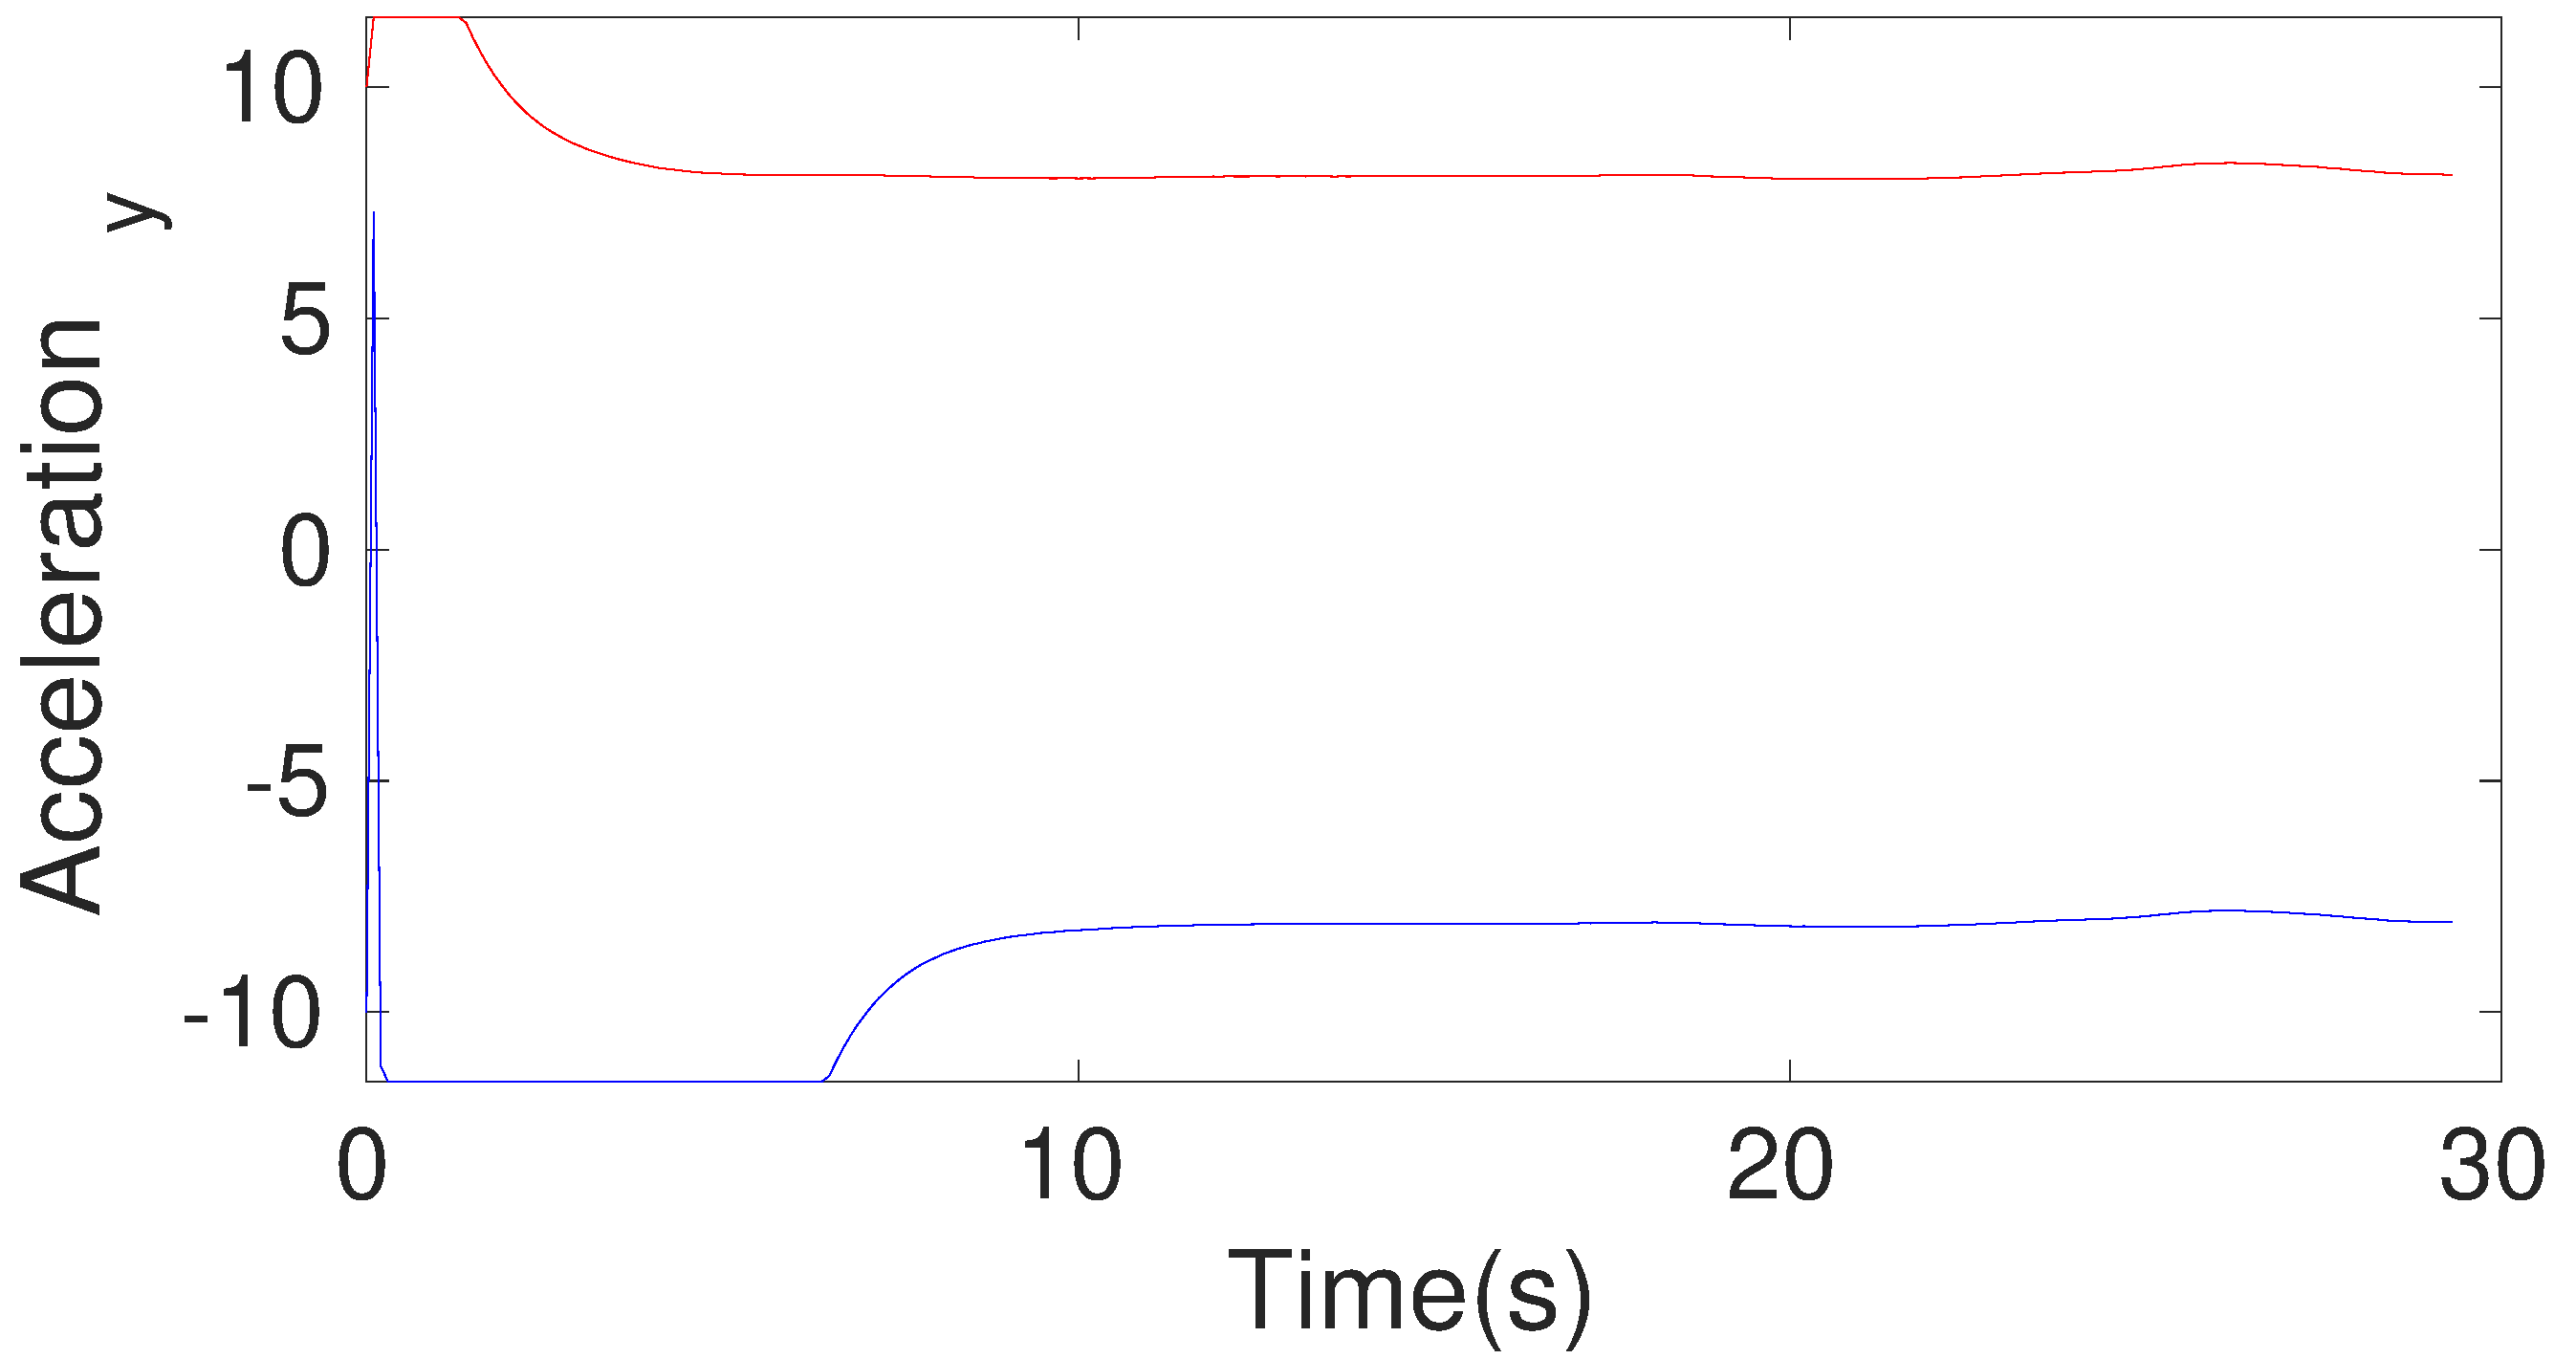
\includegraphics[width=.9\linewidth]{figures/HInf/s3pmHInfAcceleration_y}
\end{subfigure}
\caption{Estimation using Point Mass Model}
\end{figure}

\section{Rate of Change of Bounds}

\begin{figure}[h]
\begin{subfigure}{.5\linewidth}
\centering
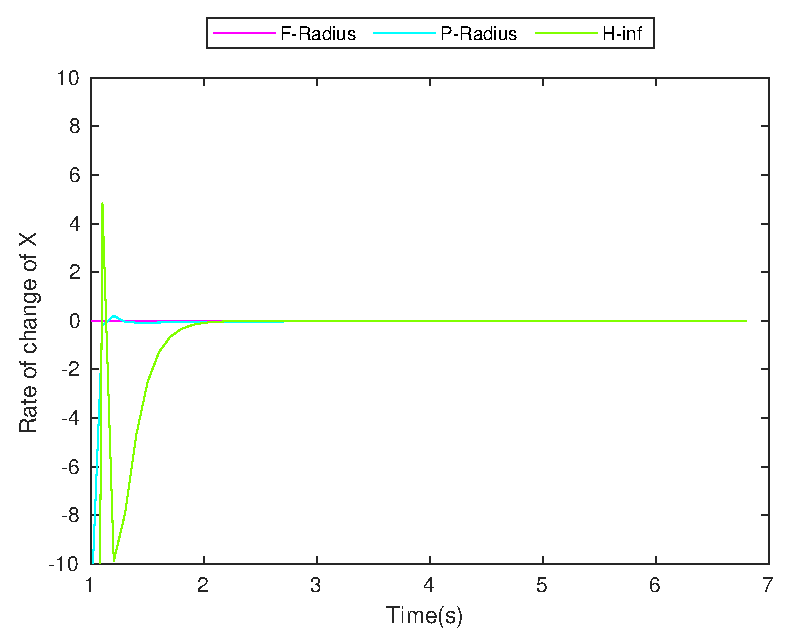
\includegraphics[width=\linewidth]{figures/BoundChange/CV/cv_bound_changeX}
\end{subfigure}
\begin{subfigure}{.5\linewidth}
\centering
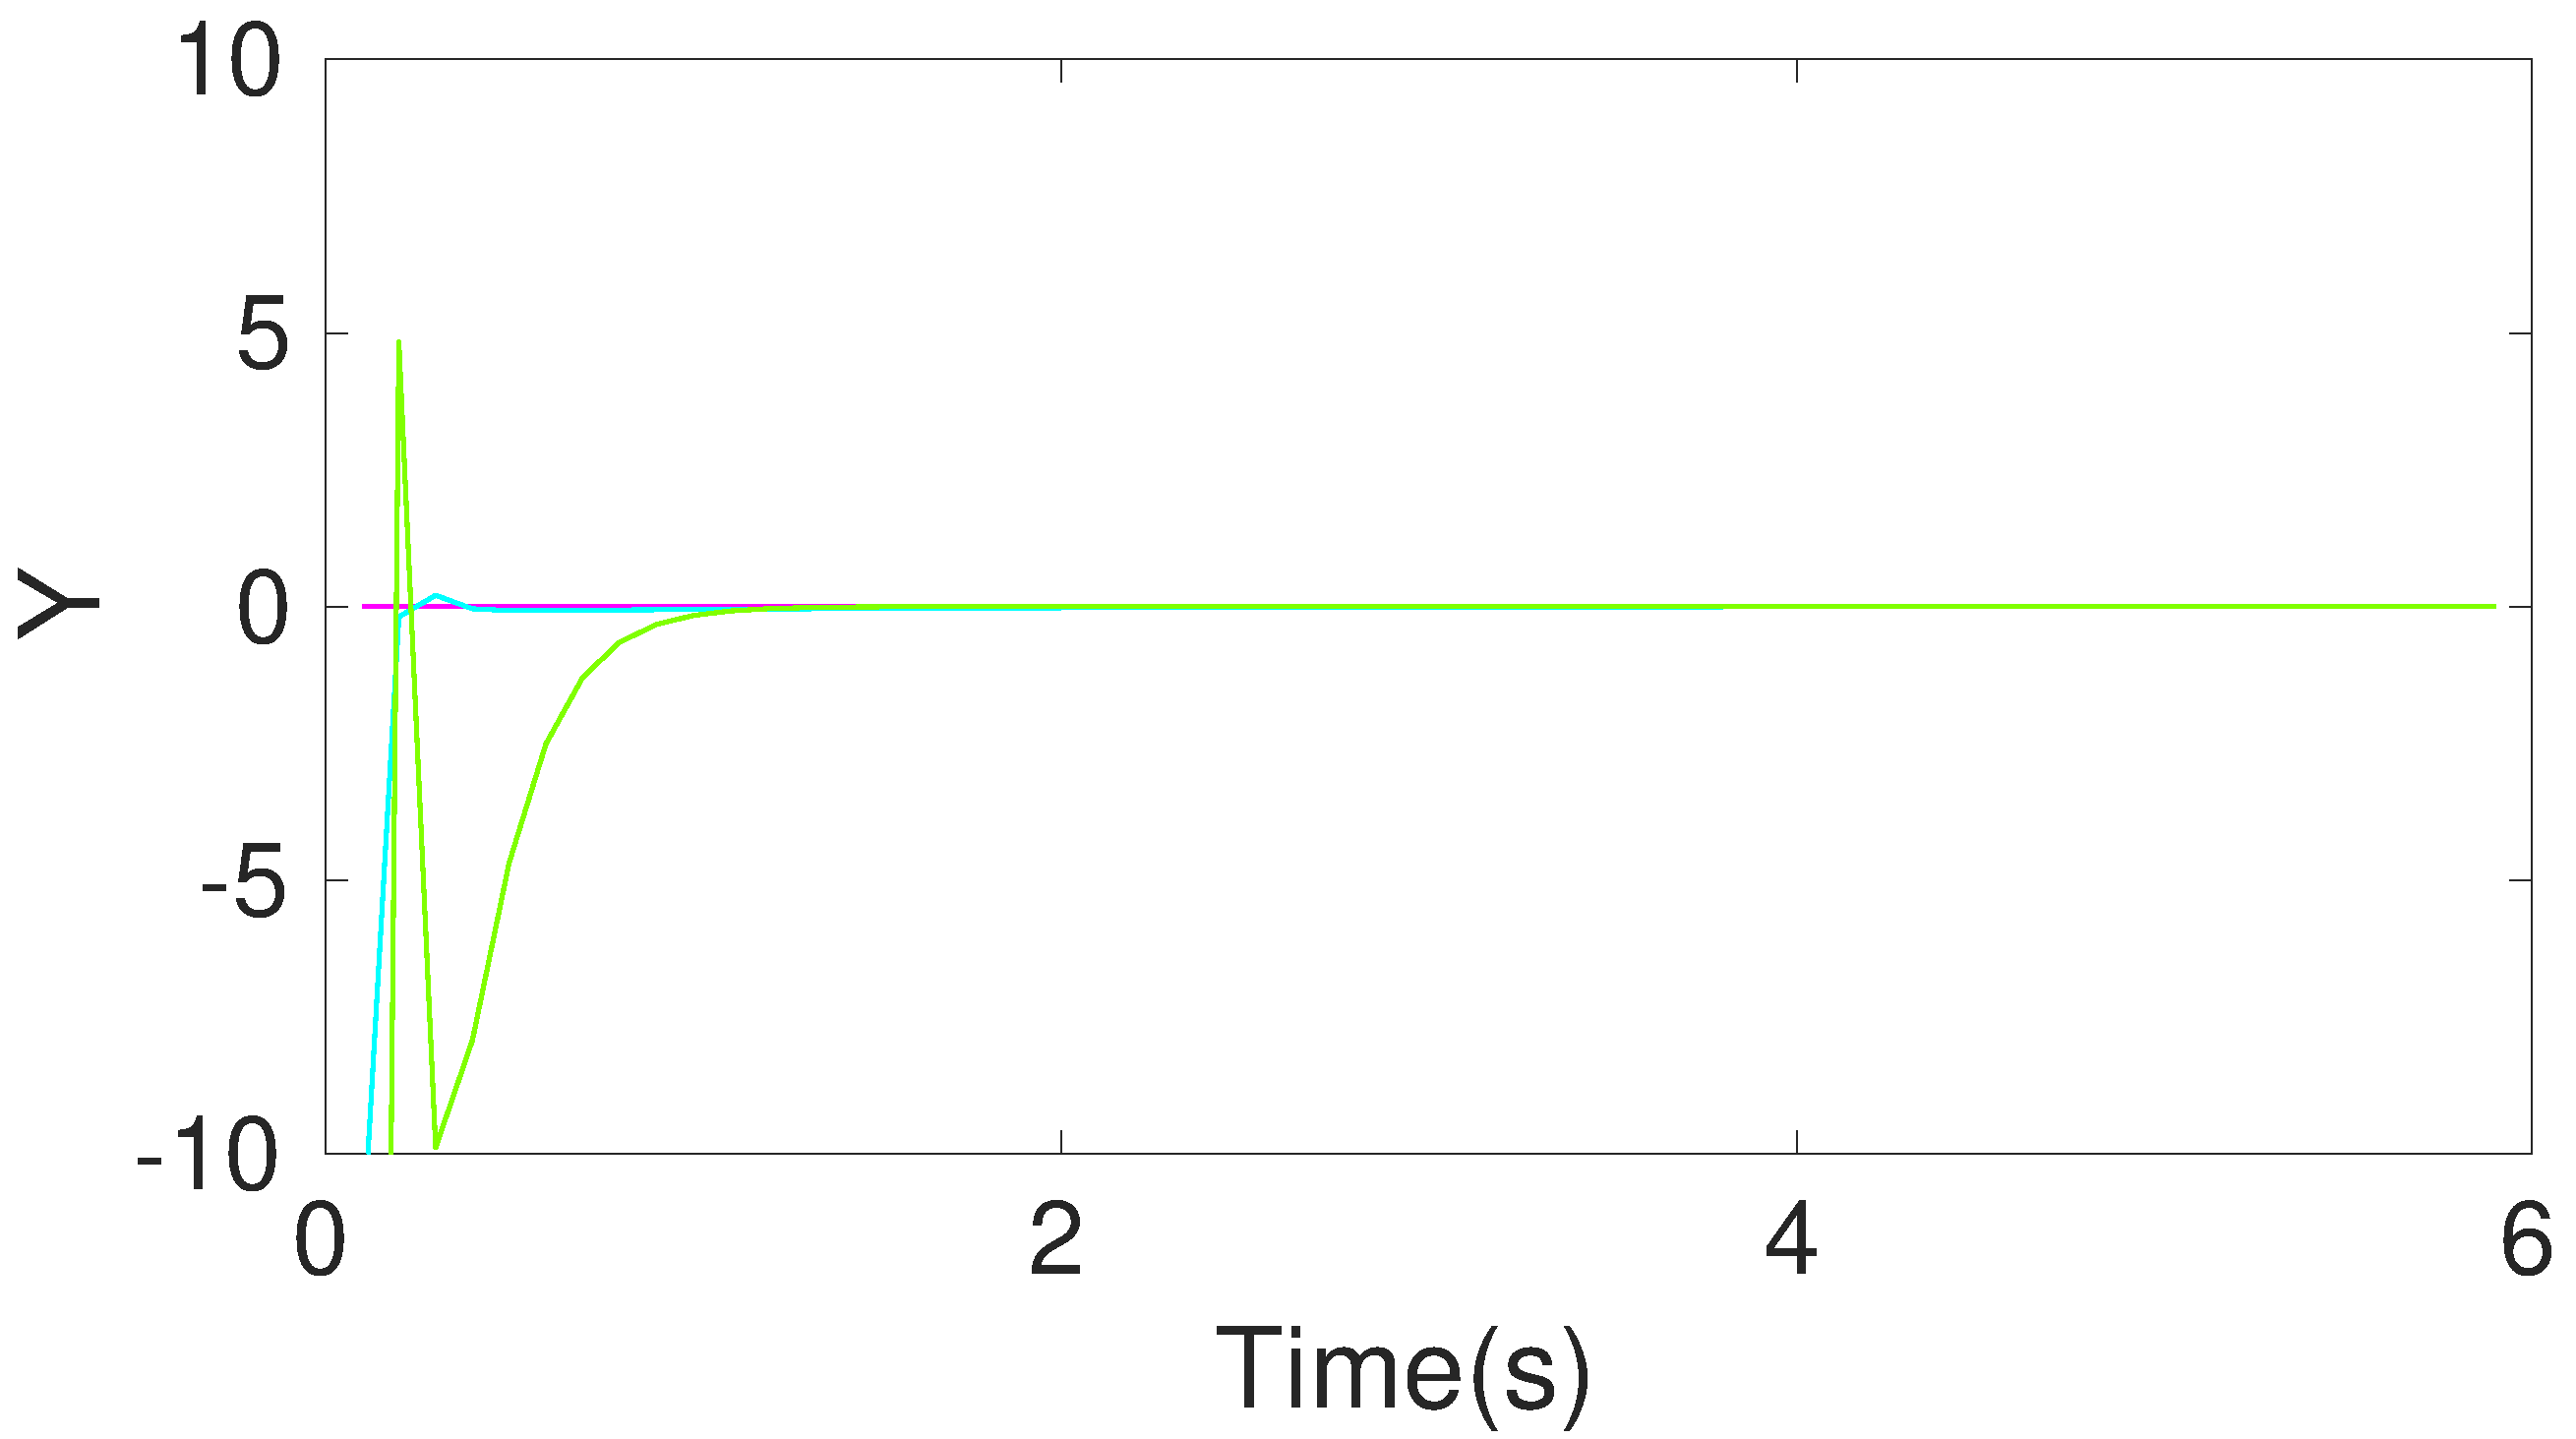
\includegraphics[width=\linewidth]{figures/BoundChange/CV/cv_bound_changeY}
\end{subfigure}
\begin{subfigure}{.5\linewidth}
\centering
\includegraphics[width=.9\linewidth]{figures/BoundChange/CV/cv_bound_changeVelocity_x}
\end{subfigure}
\begin{subfigure}{.5\linewidth}
\centering
\includegraphics[width=.9\linewidth]{figures/BoundChange/CV/cv_bound_changeVelocity_y}
\end{subfigure}
\caption{Rate of change of bounds using Constant Velocity Model}
\end{figure}


\begin{figure}[h]
\begin{subfigure}{.5\linewidth}
\centering
\includegraphics[width=\linewidth]{figures/BoundChange/CA/ca_bound_changeX}
\end{subfigure}
\begin{subfigure}{.5\linewidth}
\centering
\includegraphics[width=\linewidth]{figures/BoundChange/CA/ca_bound_changeY}
\end{subfigure}
\begin{subfigure}{.5\linewidth}
\centering
\includegraphics[width=.9\linewidth]{figures/BoundChange/CA/ca_bound_changeVelocity_x}
\end{subfigure}
\begin{subfigure}{.5\linewidth}
\centering
\includegraphics[width=.9\linewidth]{figures/BoundChange/CA/ca_bound_changeVelocity_y}
\end{subfigure}
\begin{subfigure}{.5\linewidth}
\centering
\includegraphics[width=.9\linewidth]{figures/BoundChange/CA/ca_bound_changeAcceleration_x}
\end{subfigure}
\begin{subfigure}{.5\linewidth}
\centering
\includegraphics[width=.9\linewidth]{figures/BoundChange/CA/ca_bound_changeAcceleration_y}
\end{subfigure}
\caption{Rate of change of bounds using Constant Acceleration Model}
\end{figure}

%\subsection{Singer Acceleration Model}
%\FloatBarrier
%\begin{figure}[h]
%\begin{subfigure}{.5\linewidth}
%\centering
%\includegraphics[width=\linewidth]{figures/BoundChange/CS/cs_bound_changeX}
%\end{subfigure}
%\begin{subfigure}{.5\linewidth}
%\centering
%\includegraphics[width=\linewidth]{figures/BoundChange/CS/cs_bound_changeY}
%\end{subfigure}
%\begin{subfigure}{.5\linewidth}
%\centering
%\includegraphics[width=.9\linewidth]{figures/BoundChange/CS/cs_bound_changeVelocity_x}
%\end{subfigure}
%\begin{subfigure}{.5\linewidth}
%\centering
%\includegraphics[width=.9\linewidth]{figures/BoundChange/CS/cs_bound_changeVelocity_y}
%\end{subfigure}
%\begin{subfigure}{.5\linewidth}
%\centering
%\includegraphics[width=.9\linewidth]{figures/BoundChange/CS/cs_bound_changeAcceleration_x}
%\end{subfigure}
%\begin{subfigure}{.5\linewidth}
%\centering
%\includegraphics[width=.9\linewidth]{figures/BoundChange/CS/cs_bound_changeAcceleration_y}
%\end{subfigure}
%\caption{Rate of change of bounds using Singer Acceleration Model}
%\end{figure}

\FloatBarrier
\begin{figure}[!h]
\begin{subfigure}{.5\linewidth}
\centering
\includegraphics[width=\linewidth]{figures/BoundChange/PM/pm_bound_changeX}
\end{subfigure}
\begin{subfigure}{.5\linewidth}
\centering
\includegraphics[width=\linewidth]{figures/BoundChange/PM/pm_bound_changeY}
\end{subfigure}
\begin{subfigure}{.5\linewidth}
\centering
\includegraphics[width=.9\linewidth]{figures/BoundChange/PM/pm_bound_changeVelocity_x}
\end{subfigure}
\begin{subfigure}{.5\linewidth}
\centering
\includegraphics[width=.9\linewidth]{figures/BoundChange/PM/pm_bound_changeVelocity_y}
\end{subfigure}
\begin{subfigure}{.5\linewidth}
\centering
\includegraphics[width=.9\linewidth]{figures/BoundChange/PM/pm_bound_changeAcceleration_x}
\end{subfigure}
\begin{subfigure}{.5\linewidth}
\centering
\includegraphics[width=.9\linewidth]{figures/BoundChange/PM/pm_bound_changeAcceleration_y}
\end{subfigure}
\caption{Rate of change of bounds using Point Mass Model}
\end{figure}